%!!!!!!!!!!!!!!!!!!!!!!!!!!!!!!!!!!!!!!!!!!!!!!!!!!!!!!!!!!!!!!!!!!!!!!!!!!!!!!
%!NOTE: This example file has been prepared according to the University of
%!      Hawaii Style & Policy Manual for Theses and Dissertations dated
%!      "Revised February 1998". If you have one with a later date, you may
%!      need to make revisions to this document as well. In any event, making
%!      sure your thesis complies with Graduate Division guidelines is
%!      ultimately your responsibility. Caveat LaTeXtor. :)
%!!!!!!!!!!!!!!!!!!!!!!!!!!!!!!!!!!!!!!!!!!!!!!!!!!!!!!!!!!!!!!!!!!!!!!!!!!!!!!

%% The options are (you can only choose one from each group):
%%
%% 10pt, 11pt, 12pt: chooses the point size for the document. "11pt" is the
%%                   default.
%%
%% oneside, twoside: whether you want your document onesided or twosided. Note
%%                   that twosided is not guaranteed to work, and style
%%                   guidelines prohibit double sided printouts on final
%%                   copy. "oneside" is the default.
%%
%% draft, final: when printing drafts you can save a lot of paper by using the
%%               "draft" option. It switches to single spacing, displays overful
%%               hboxes with a black box, prints a version number on title page 
%%               and omits signature page. Of course for the final copy make
%%               sure to use the "final" option! "final" is the default.
%%
%% cm, times, palatino, newcent, bookman: switches between different font
%%                                        sets. "cm" is the Computer Modern
%%                                        font (TeX's default), the rest are
%%                                        PostScript fonts. "times" is the
%%                                        default.
%%
%% thesis, dissertation: switches between the style for a master's thesis and a 
%%                       Ph.D. dissertation. The differences are fairly minor
%%                       and limited to the front matter. "thesis" is the
%%                       default.
%%
%% actual, proposal: switches between actual document and proposal mode. In
%%                   proposal mode: the title page is simplified, the
%%                   version number is always printed, and the signature page
%%                   is omitted.
%%
%%% Load the uhthesis2e document class
\documentclass[11pt,final,times,dissertation,actual]{uhthesis2e}
%\documentclass[11pt,draft,times,dissertation,proposal]{uhthesis2e}

%% hyperref package complains if this isn't here. Might be unneeded when
%% I switch to the new UH thesis style
\paperheight = 11in

%%% Load some useful packages:
%% New LaTeX2e graphics support
\usepackage{graphicx}
%%	using final option to force graphics to be included even in draft mode
%\usepackage[final]{graphicx}
%% Tell graphicx the default directory for all figures
\graphicspath{{figures/final/}}

%% Enable subfigure support
\usepackage{subfigure}

%% Make subsubsections numbered and included in ToC
\setcounter{secnumdepth}{3}
\setcounter{tocdepth}{3}

%% Package to linebreak URLs in a sane manner.
\usepackage{url}

%% Define a new 'smallurl' style for the package that will use a smaller font.
\makeatletter
\def\url@smallurlstyle{%
  \@ifundefined{selectfont}{\def\UrlFont{\sf}}{\def\UrlFont{\small\ttfamily}}}
\makeatother
%% Now actually use the newly defined style.
\urlstyle{smallurl}

%% Define 'tinyurl' style for even smaller URLs (such as in tables)
\makeatletter
\def\url@tinyurlstyle{%
  \@ifundefined{selectfont}{\def\UrlFont{\sf}}{\def\UrlFont{\scriptsize\ttfamily}}}
\makeatother

%% Provides additional functionality for tabular environments
\usepackage{array}

%% Set up to create an index
\usepackage{makeidx} 
\makeindex

%% Puts space after macros, unless followed by punctuation
\usepackage{xspace}

%%% Personal macros
%% Tired of typing CO2 so many times, requires xspace package
\newcommand{\COtwo}{CO\ensuremath{_2}\xspace}
%% Hawai`i with okina
\newcommand{\Hawaii}{Hawai`i\xspace}
%% Manoa with kahako
\newcommand{\Manoa}{M\=anoa\xspace}

%% Provides customization of lists
\usepackage{enumitem}

%% Now define question list type
\newlist{question}{enumerate}{1}
\setlist[question]{resume, label=\textbf{\arabic*.}}

%% Define multiple choice answer list type
\newlist{answer}{enumerate}{1}
\setlist[answer]{label=\alph*)}

%% Allows insertion of fixme notes for future work
%% Note, remove status=draft when printing final version!
\usepackage[footnote, nomargin, status=final]{fixme}
%\usepackage[footnote, nomargin, status=draft]{fixme}
%% turned off marginclue because it generates hbox overflows for each note :(
%\usepackage[footnote, nomargin, marginclue, status=draft]{fixme}

%% Make URLs clickable
\usepackage[colorlinks, citecolor=blue, bookmarks=false]{hyperref}
%\usepackage[colorlinks, citecolor=blue, bookmarks=true, backref]{hyperref}

%% Make \autoref from hyperref package capitalize things normally
\def\chapterautorefname{Chapter}
\def\sectionautorefname{Section}

%% Make links to captions point to the figure, not just the caption at bottom
\usepackage[all]{hypcap}

%% Set up to create a glossary
%\usepackage[toc]{glossaries}
%\makeglossaries

%% Since I'm using the LaTeX Makefile that uses dvips, I need this
%% package to make URLs break nicely
\usepackage{breakurl}

% correct bad hyphenation here
\hyphenation{strong-ly}

%%% End of preamble
\begin{document}

%%% Declarations for Front Matter. Capitalize all of these values
%%% "normally". This allows the document class to format them properly.
%% Full title of thesis or dissertation, capitalized like a title should be.
\title{Fostering Sustained Energy Behavior Change and Increasing Energy Literacy In A Student Housing Energy Competition}
%% Your name, capitalized normally. Do not include any titles like Dr.
\author{Robert S. Brewer}
%% Month in which you intend to receive your degree (i.e. graduation).
%% Presumably this will be one of: May, August, or December.
\degreemonth{May}
%% Year of expected graduation.
\degreeyear{2010}
%% Type of degree to be conferred.
\degree{Doctor of Philosophy}
%% This is the chairperson of your committee. Do not use titles like Dr.
\chair{Philip M. Johnson}
%% The other members of your committee, seperated by "\\". Again, no titles,
%% and it is customary to list the outside committee member (if you have one)
%% last.
\othermembers{Martha E. Crosby\\
Scott Robertson\\
Daniel D. Suthers\\
Anthony Kuh}
%% This is the total size of your committee, including the chairperson. The
%% signature page routine will only handle up to 6 members; if you have more
%% than that you will need to modify the document class.
\numberofmembers{5}
%% The field in which you are obtaining your degree, capitalized normally.
\field{Computer Science}
%% The version number of your document. Consistent use of this will enable you
%% to tell old drafts from new ones. Final actual documents omit this
%% automatically so you can use it without fear of submission problems at the
%% end. If you do not define this parameter, it defaults to "1.0.0".
\versionnum{1.0.0}

%%% Create the title page from all the information above. Note that the
%%% titlepage is outside the front matter.
\maketitle

\begin{frontmatter}

%%% Create the signature page (when indicated by the options)
\signaturepage

%%% Create the copyright page
%\copyrightpage

%%% Bring in the dedication page from external file
%%%%%%%%%%%%%%%%%%%%%%%%%%%%%%% -*- Mode: Latex -*- %%%%%%%%%%%%%%%%%%%%%%%%%%%%
%% uhtest-dedication.tex -- 
%% Author          : Robert Brewer
%% Created On      : Fri Oct  2 16:29:01 1998
%% Last Modified By: Robert Brewer
%% Last Modified On: Fri Oct  2 16:29:20 1998
%% RCS: $Id: uhtest-dedication.tex,v 1.1 1998/10/06 02:07:25 rbrewer Exp $
%%%%%%%%%%%%%%%%%%%%%%%%%%%%%%%%%%%%%%%%%%%%%%%%%%%%%%%%%%%%%%%%%%%%%%%%%%%%%%%
%%   Copyright (C) 1998 Robert Brewer
%%%%%%%%%%%%%%%%%%%%%%%%%%%%%%%%%%%%%%%%%%%%%%%%%%%%%%%%%%%%%%%%%%%%%%%%%%%%%%%
%% 

\begin{dedication}
\null\vfil
{\large
\begin{center}
To myself,\\\vspace{12pt}
Perry H. Disdainful,\\\vspace{12pt}
the only person worthy of my company.
\end{center}}
\vfil\null
\end{dedication}


%%% Bring in the acknowledgements section from external file
%%%%%%%%%%%%%%%%%%%%%%%%%%%%%%% -*- Mode: Latex -*- %%%%%%%%%%%%%%%%%%%%%%%%%%%%
%% uhtest-acknowledgements.tex -- 
%% Author          : Robert Brewer
%% Created On      : Fri Oct  2 16:29:43 1998
%% Last Modified By: Robert Brewer
%% Last Modified On: Fri Oct  2 16:29:52 1998
%% RCS: $Id: uhtest-acknowledgements.tex,v 1.1 1998/10/06 02:06:54 rbrewer Exp $
%%%%%%%%%%%%%%%%%%%%%%%%%%%%%%%%%%%%%%%%%%%%%%%%%%%%%%%%%%%%%%%%%%%%%%%%%%%%%%%
%%   Copyright (C) 1998 Robert Brewer
%%%%%%%%%%%%%%%%%%%%%%%%%%%%%%%%%%%%%%%%%%%%%%%%%%%%%%%%%%%%%%%%%%%%%%%%%%%%%%%
%% 

\begin{acknowledgements}
I want to ``thank'' my committee, without whose ridiculous demands, I
would have graduated so, so, very much faster.
\end{acknowledgements}


%%% Bring in the abstract section from external file
%%%%%%%%%%%%%%%%%%%%%%%%%%%%%% -*- Mode: Latex -*- %%%%%%%%%%%%%%%%%%%%%%%%%%%%
%% uhtest-abstract.tex -- 
%% Author          : Robert Brewer
%% Created On      : Fri Oct  2 16:30:18 1998
%% Last Modified By: Robert Brewer
%% Last Modified On: Fri Oct  2 16:30:25 1998
%% RCS: $Id: uhtest-abstract.tex,v 1.1 1998/10/06 02:06:30 rbrewer Exp $
%%%%%%%%%%%%%%%%%%%%%%%%%%%%%%%%%%%%%%%%%%%%%%%%%%%%%%%%%%%%%%%%%%%%%%%%%%%%%%%
%%   Copyright (C) 1998 Robert Brewer
%%%%%%%%%%%%%%%%%%%%%%%%%%%%%%%%%%%%%%%%%%%%%%%%%%%%%%%%%%%%%%%%%%%%%%%%%%%%%%%
%% 

\begin{abstract}
Abstract goes here, and will be written once the proposal is mostly done.
\end{abstract}


%%% Generate list of FiXmes, will be silent in final mode
\listoffixmes

%%% Generate table of contents
\tableofcontents

%%% Generate list of tables
\listoftables

%%% Generate list of figures
\listoffigures


\end{frontmatter}

%%% Include each chapter
\chapter{Introduction}\label{chapter_introduction}
\textit{The central issue I address in the dissertation is a possibility of recurrent behaviors discovery from 
publicly available software process artifacts by leveraging data mining and knowledge discovery techniques. 
In particular I explored an approach of discovering of recurrent behaviors through the mining of time series that
are constructed by temporal ordering of measurements extracted from software process artifacts.
Further, I shall propose a novel technique for characteristic patterns discovery from time series and show its 
applicability to the problem at hands.}

\textit{The problem's background is provided in the Section \ref{section_background}. 
Section \ref{section_software_process_design} presents classical approaches for software process design and shows its limitations.
Section \ref{section_research_hypothesis} introduces the research hypothesis.
Section \ref{knowledge_discovery} provides a background into the problem of knowledge discovery 
from time-series.
Section \ref{section_trajectory_definition} connects two problems and provides definitions.
Section \ref{section_contributions} enumerates main contributions of the thesis, 
while section \ref{section_organization} explains the thesis organization.}

%
% >> section
%
\section{Background}\label{section_background}
Contemporary software projects concern with development of complex software systems and typically have 
a considerably long life-cycle - well over decade.
A project's development and maintenance activities are usually carried out by geographically 
distributed teams and individuals. The development pace, the experience, and the structure of the 
development team continuously change with project progression and as developers joining and leaving. 
When combined with schedule and requirements adjustments, these create numerous difficulties 
for developers, users, and stakeholders, ultimately affecting the project success \cite{citeulike:2207657}. 

This software development complexity phenomena was identified in 1968 as ``Software crisis'' 
\cite{naur_crisis_68}, and was addressed by bringing the research and the practice of software development 
(or as it was called ``programming'') under the umbrella of Engineering - in an effort to provide 
the control over the process of software development. 
Following the engineering paradigm, numerous methodologies and models of software design and development 
process, known as \textit{software processes}, were proposed \cite{citeulike:10002165}.

\begin{defn}\label{def_process}
A \textbf{\textit{Software Process}} defines a sequence of activities performed in order 
to design, develop, and maintain software systems.
\end{defn}
Examples of such activities include requirements collection and creation of UML diagrams, 
requirements testing, code development,  testing, etc. The intent behind a software process is 
to provide a control over software evolution by implementing a global strategy and by structuring
and coordinating human activities in order to achieve the goal - deliver a functional software system 
on time and under the budget. 

Since then, much research has been done on software processes resulting in a number
of software development models and paradigms. Some of these were widely accepted by practitioners 
and evolved into industrial standards for software development processes such as CMM, ISO, PSP, 
and others \cite{citeulike:5043104}. However, in spite of this effort, industrial software 
development remains error-prone and more than half of all 
commercial software development projects ending up failing or being very poorly executed 
(Rubinstein, ``Chaos Reports'', 2006) \cite{chaos2006}. Some of them are abandoned due to running 
over budget, some are delivered with such low quality, or so late, that they are useless, and some, 
when delivered, are never used because they do not fulfill requirements. 

Through the analyses of software project failures, it was acknowledged, that the engineering 
paradigm might not be the best way to provide a control over software development processes 
(\cite{citeulike:3729379} \cite{citeulike:5203446}) due to the fact that Software engineering 
is dealing with significantly different from other Engineering fields problems \cite{citeulike:2207657} .
The chief argument supporting this point of view is the drastic difference in the cost model:
while in Software Engineering there is almost no cost associated with materials and 
fabrication, these usually dominate cost in all other Engineering disciplines, but, 
ironically, Software Engineering is suffering from the costs and challenges associated with 
continuous re-design of the product and its design processes - the issue which is 
hardly seen at all in other Engineering areas. 
Further, it was found, that most of the engineering-like models are rigid, ``context-free'',
and rather prescriptive, i.e. they are universally defined independently of a particular 
organizational structure or a project specificities \cite{sacchi_2001}, and while they 
structure processes and provide the control, following them does not guarantee the success.
Yet another argument supporting alternative to engineering approaches is the increasing 
understanding and appreciation of a human role in software development processes over tools, 
technologies, and standards \cite{citeulike:6580825} \cite{citeulike:149387}
\cite{1605185} \cite{citeulike:113403} \cite{1605188} \cite{citeulike:12743107}. 

Along with Software Engineering, a number of alternative, flexible and user-oriented software processes 
emerged from academy, hobbyists, and practitioners addressing aforementioned issues \cite{citeulike:3729379}. 
Among others, the Free/Libre/Open-Source Software model (FLOSS) and the software craftsmanship  
approaches gained a significant credibility in community. 
While the former \textit{holistic} software process paradigm emphasizes loosely-organized 
collaboration, frequent releases, and effectively removes the boundary between developers 
and customers, the latter, human-centric approach, is built upon the roles of highly 
motivated skilled individuals \cite{citeulike:262020} \cite{citeulike:2759198}. 

Nevertheless, alternative processes were found to be plagued by the same complexity issues. 
As it was shown, most of FLOSS projects never reach a ``magic'' 1.0 version \cite{citeulike:12480029}. 
Among others, the great "infant mortality rate" of FLOSS projects was related to a burnout, 
inability to acquire a critical mass of users, loss of leading developer(s), and forking \cite{richter2007critique}. 
Software craftsmanship, from other hands, not only challenges developers with technological advances 
requiring continuous skills improvement, but creates significant cost and effort estimation difficulties for
stakeholders and project managers \cite{citeulike:11058784}. However, despite to these issues, 
the alternative processes proved that the disciplined manner of programming and the modularization  
of the software are capable of delivering large and reliable software systems, most notable Linux OS,
suggesting that community-driven processes as good as industrial engineering-like processes.

Currently, it is widely acknowledged, that there exists no single ``silver bullet'' process which 
can bring a software development project to success \cite{citeulike:1986013}. 
Processes are numerous, each has advantages and drawbacks, and each is accompanied with 
numerous application recommendations, success stories, and with failure experiences. Nevertheless,
the alarming rate of failing projects suggests that our understanding of software process ``mechanics''  
is limited and insufficient\cite{citeulike:12550665}. 
The enormous cost of the lost effort, measured in hundreds of billions of US dollars 
\cite{citeulike:2207657} \cite{citeulike:2207653} \cite{citeulike:2207655}, 
continues to provide motivation for further research on software processes. 

%
% >> section
%
\section{Software process design}\label{section_software_process_design}
Traditionally, approaches to software process design and improvement are divided into two distinct categories. 

The first category of software process design approaches consists of traditional to engineering 
\textit{top-down} prescriptive techniques through 
\textit{proposing a process based on specific patterns of software development}. 
For example, the Waterfall Model process proposes a sequential pattern in which developers first create a 
Requirements document, then create a Design, then create an Implementation, and finally develop Tests. 
The Test Driven Development process, from other hands, proposes an iterative behavioral pattern in which
the developer must first write a test case, then write the code to implement that test case, then re-factor the 
system for maximum clarity and minimal code duplication \cite{citeulike:6086365}. 

While the top-down approach follows the usual path of trials and errors, and seems to be an extension 
of natural to humans creative processes of invention and experimentation, 
the ``invention'' of an adequate to the task software process is far from trivial 
\cite{citeulike:5043104} \cite{citeulike:1986013}. Moreover, an evaluation cycle of an invented process
is usually very expensive and considerably long.
In addition, it was shown that the process inventors are often limited in their scope and tend to assume 
idealized versions of real processes, thus, often produce ``paper lions'' - process models which are 
likely to be disruptive and unacceptable for end users, at least in their proposed form 
\cite{citeulike:9758924}, which creates a large discrepancy between actions that supposed to be done for 
the novel process and what was actually performed by particular individual or the team.

The second category of software design approaches consists of \textit{bottom-up} techniques 
that focus on a \textit{performed process reconstruction through noticing of recurrent development 
events and behaviors} or as it also called \textit{process enactment}. 
Usually, the process reconstruction task is viewed as a two-levels problem where the first level 
consists of a patterns discovery (segmentation) while the second level consists of patterns recognition 
and their network analysis \cite{citeulike:2703162}.
One of the first works in this category was by Cook and Wolf, where they show a
possibility of automated extraction of a process model through the mining of recorded 
process event logs \cite{citeulike:328044} \cite{citeulike:5120757} \cite{citeulike:5128143}. 
Later work by Huo et al. shows that it is also possible to improve an existing process
through the event logs analysis \cite{citeulike:7691059} \cite{citeulike:7690766}. 

While the bottom-up approaches seem to be more systematic and potentially less complex than invention, 
they also affected by a number of issues. A chief among these is the observability issue - 
it is usually very difficult to conduct a full depth study on a live project due to the privacy concerns. 
Moreover, it is expensive to observe a process performed by a team for a whole life-cycle of a project. 
Yet another issue is the capacity of currently available process discovery techniques - 
typically these need to be supervised by experts and finely tuned in order to reconstruct 
distributed and concurrent processes. 

Nevertheless, despite to their differences, both techniques for software process design are 
producing process models that effectively are the series of actions that must be performed successively 
(sequentially and sometimes iteratively) in order to deliver a software. 
In order to produce the viable model, the ``process inventors'' put the best of their knowledge, experience,
creativity, and logical reasoning into the proposed sequence of steps, while ``process re-constructors 
strive to eliminate the noise and to converge to a concise process model that is supported by the 
majority of observations. 
This attention to synthesis of sequential steps, leaves other phenomenas, such as team's structure, work schedule, 
developer's discipline, their behaviors, and motivation behind. While this issue was recognized previously
and resulted in a number of studies which called for attention of human element in software production 
\cite{citeulike:149387} \cite{citeulike:113403} \cite{citeulike:205322} \cite{citeulike:12798652}, 
it is still largely ignored in industrial practices \cite{citeulike:12798659}, mostly due to the 
difficulties in benefit estimation \cite{citeulike:12798662} \cite{csdl2-12-11}.

%
% >> section
%
\section{Free/Libre Open Source processes}\label{floss_processes}
Along with growing amount of publicly available software, it became obvious, that self-organizing communities of 
mostly ``recreational'' software developers and active users are capable to successfully manage large code base, 
but to deliver software increasingly complex and surprisingly popular.
Many of large, ``global'' open source software development projects, such as Linux and its derivatives, 
Gnome, Apache HTTP Server, MySQL, and others, not only have comparable with industrial projects development team 
and code-base sizes, but the same average defect rate \cite{coverity2012}. 
These facts have attracted a considerable attention from industry and many organizations 
seek to emulate successful open source software processes in traditional ``closed source'' environment 
\cite{oss_virtual_organizations} \cite{oss_balance} \cite{oss_hp} \cite{oss_4industry}. 

\begin{figure}[ht!]
   \centering
   \includegraphics[width=140mm]{figures/Linus.Kernel.ps}
   \caption{A Torvald's response suggesting that practical reasons, the ``real-life'', should be always considered 
   over specifications.
   Excerpt from the Linux mailing list. \url{http://lkml.indiana.edu/hypermail/linux/kernel/0509.3/1441.html}}
   \label{fig:kernel}
\end{figure}

If we consider this as an assertion that open-source software processes are at least as good as engineering-like 
software process models, then, the freely available open-source process software artifacts potentially bear an 
incredible wealth of the information worth of studying. Moreover, the striking differences of open-source processes 
from a traditional software development could potentially reveal novel software processes and their aspects that 
were previously not accounted for. 
For example, consider that the most significant document in industrial software processes - a specification - 
is rarely considered at all in open source world. In FLOSS projects the software look and its functionality are 
rather viewed as open-end questions. Even in the Linux kernel development, which is probably one of the few strictly 
moderated FLOSS development processes, developers prise practical reasons over specifications 
\ref{fig:kernel}.

Yet another source of motivation for studying of public FLOSS software process artifacts comes from the fact that 
in order to facilitate the distributed FLOSS software development processes, the community is highly encouraging
developers to commit their changes rather often \cite{so-checkin} \cite{git-best-practices1}.
The frequent commits and the changes visibility practice is often cited as vital for health of software 
process as mentioned in some lengthy discussions: ``\textit{Don't Go Dark}'' \cite{checkin-dgd-2008}, 
``\textit{Check In Early, Check In Often}'' \cite{checkin-ch-2012}. Potentially, frequent commits create artifacts 
trails that provide finer resolution into project development and allow more thorough process recovery.

%
% >> section
%
\section{Public software repositories}\label{section_public_repositories}
Recently, the aforementioned situation changed, and the interest for process enactment and reconstruction, 
as well as attention to the human-specific components of software processes has been revived. 
This change is driven by the increase in public data that are made available by the proliferation of open 
source communities.

Currently, with accessible personal computers, friendly software development toolkits, and due to massification
of the use of the web as
a platform for collaborative work, small-scale commercial and recreational 
programming become very popular. 
Today, free code hosting sites such as SourceForge, GoggleCode, and GitHub host thousands of 
Free/Libre Open Source Software (FLOSS) projects.
These publicly offer numerous software artifacts such as design documents, source codes, bugs and issue records, and 
developers and users communications.
Further, Q\&A and social websites for developers such as StackOverflow, Biostars, TopCoder and others becoming 
increasingly popular among the software developers as places for exchanging experiences, learning new tricks, and 
improving skills, plus, they offer anonymized data back to the community.

The public availability of numerous software process artifacts effectively removes not only the high cost of observation, 
but most of the privacy concerns - the two issues that previously made any large-scale analysis of software projects 
unfeasible for most researchers.

Scientific community response on the availability of public artifacts was overwhelming, and a number of 
venues was established addressing the increased interest. 
Since 2004, the International Conference on Software Engineering (ICSE) hosts a Working Conference on 
Mining Software Repositories (MSR). The original call for papers stated MSR's purpose as 
\textit{``... to use the data stored in these software repositories to further understanding of software 
development practices ... [and enable repositories to be] used by researchers to gain empirically based 
understanding of software development, and by software practitioners to predict and plan various aspects 
of their project''} \cite{msr2004} \cite{citeulike:7853299}. 
Several other venues: International Conference on Predictive Models in Software Engineering \cite{promise12}, 
International Conference on Open Source Systems, the Workshop on Public Data about Software Development, 
and the International Workshop on Emerging Trends in FLOSS Research have also played
an important role in shaping and advancing this research domain.

Some of the published work addresses the software process discovery. Among others, most notable and 
relevant to my research is work by Jensen \& Scacchi. In their early work, they demonstrated, that 
information reflecting software processes can be gathered from public systems \cite{citeulike:12550640}. 
Later, in \cite{citeulike:5043664} and \cite{citeulike:5128808}, they show, that by manual mapping of 
collected process evidence to a pre-defined process meta-model it is possible to reconstruct some 
of the FLOSS processes. 
Another closely related to my research is work by Hindle et al. where they has shown that it is possible to 
discover software process evidence through partitioning \cite{citeulike:10377366}.

However, the research work based on mining of software process artifacts shows, that while public availability 
of artifacts is minimizing observability and privacy issues, the nature of these artifacts creates a number of 
challenges which I discuss in the chapter X, which limit the possible scope of the research and significantly 
elevate the complexity of the process discovery effectively rendering previously designed techniques inefficient.
Thus, the novel analysis and discovery techniques are needed to be developed for public software process artifacts 
analysis \cite{citeulike:7853299}.
% when ``\textit{... going beyond code and bugs...}'' 

%
% >> section
%
\section{Research hypothesis, scope of the dissertation}\label{section_research_hypothesis}
In previous sections, I have outlined the evidence of a limited performance of existing engineering-like 
software processes (Section \ref{section_background}),
as well the oversight of a variety of human factors that fall beyond a typical sequence of development 
actions by traditional approaches to software process design (Section \ref{section_software_process_design}).
Then, I have identified a few differences of FLOSS processes from traditional Software Engineering 
(Section \ref{floss_processes}), which can potentially shed light on human-driven aspects of software development.
Finally, I have pointed out a growing wealth of publicly available software process artifacts 
(Section \ref{section_public_repositories}) that is worth to explore for a better understanding not only 
FLOSS software processes, but their human factors. All this provided a motivation to my exploratory study, 
whose details I outline in this section.

In my work, I attempted to explore the possibility of discovery of a specific human-driven aspect in 
FLOSS software development that is a \textit{\textbf{behavior}}, which I define as the mannerism in which a 
developer, or a team, conduct their everyday work. 
In particular, I explore the possibility of discovery of \textit{recurrent behaviors}, i.e. behaviors supported 
by a numerous evidence, from software process artifacts. 

For example, if within an observation interval one developer frequently runs unit tests before committing 
changes into repository, while another usually commit changes without running the tests, the first developer's
habit of testing a code before the commit is a recurrent behavior that may reflect the developer's discipline,
or an unusual attention to some particular part of the code. 
Consider another example, if one of the developers usually commits code changes in mornings, while another 
developer late in the day, these two recurrent behaviors, might indicate a constraints that are put on the 
project, or the process, or on the developers themselves.
Obviously, latter behaviors should be possible to quantify by simple analysis of commit timestamps, while 
the former can be discovered by the analysis of co-occurring changes in the source code. 
Moreover, these and similar recurrent behaviors could be further associated with certain project's or process 
traits, such as pace, agility, size, complexity, code quality and others, which will not only extend our 
knowledge of human factors in software processes, but will lay a foundation for future research in software 
processes.

To begin with, I hypothesized, that \textbf{\textit{it is possible to discover recurrent behaviors from 
publicly available software process artifacts}}. 

Following the hypothesis, I have investigated a number of publicly available software repositories,
their artifacts, and a number of applicable data-mining techniques in a preliminary exploratory study 
\cite{csdl2-10-09}. However, similarly to other studies in the field, I have discovered, that while FLOSS 
process artifacts are numerous and readily accessible, their irregular, snapshot-like nature and the poor 
informational content significantly limit the applicability of known techniques for process mining.

In order to overcome this issue, I have casted the initial problem of event-based recurrent behaviors 
discovery into more generic problem of knowledge discovery from time series and approached it
by developing a novel technique for interpretable comparative analysis of time series that allows 
characteristic patterns discovery and ranking called SAX-VSM \cite{sax-vsm}. 

Further, I have developed a software artifacts analysis framework, called Software Trajectory Analysis, 
which aids in software artifacts collection, software process and product evolutionary metrics extraction, 
and their comparative analyses that enable discovery and ranking of characteristic patterns.


 in rank highlight is  transformation into  and by using I approached the problem of knowledge discovery 

developed a 
software process artifacts mining framework called Software Trajectory Analysis which is built upon 
a novel technique for comparative analysis of time series that allows characteristic patterns discovery 
and ranking.

This dissertation presents its results, as well as introduces a novel data mining technique designed to 
alleviate difficulties with interpretability of quantitative results obtained through mining of software
artifacts trails. 

%
% >> section
%
\section{Knowledge discovery from time series}\label{section_knowledge_discovery}
In data mining, time series are used as a proxy representing a vast variety of real-life phenomena 
in wide range of fields including, but not limited to physics, medicine, meteorology, 
music, motion capture, image recognition, signal processing, and text mining. 
While time series usually directly represent observed phenomenas by capturing their measurable evolution in time, 
the pseudo time series often used for representation of various high-dimensional data 
by combining data points into ordered sequences. 
For example in spectrography data values are ordered by component wavelengths \cite{citeulike:12550833};
in shape analysis the order is the clockwise walk direction starting from a
specific point in the outline \cite{citeulike:12550835}, in image classification the numbers of pixels
are sorted by color component values \cite{citeulike:2900542}.

Many important problems of knowledge discovery from time series reduce to the core task of finding 
characteristic, likely to be repeated, sub-sequences in a longer time series. 
In the early work these were called as 
\textit{frequent patterns} \cite{citeulike:5159615}, 
\textit{approximate periodic patterns} \cite{citeulike:1959582},
\textit{primitive shapes} \cite{citeulike:5898869}, 
\textit{class prototypes} \cite{citeulike:4406444}, 
or \textit{understandable patterns} \cite{citeulike:3978076}. 
Later, similarly to Bioinformatics, these were unified under the term \textit{motif} \cite{citeulike:3977965}.
Once found, motifs can be used for a hypothesis generation by finding their associations with known,
or unknown phenomenas \cite{citeulike:3977965}. 

The recent advances in semi-supervised and unsupervised finding of such characteristic sub-sequences, 
in particular work based on \textit{shapelets} \cite{citeulike:7344347} \cite{citeulike:11957982}
\cite{citeulike:12552293} and \textit{bag of patterns} \cite{citeulike:10525778}, show a great potential 
of application of time series data-mining techniques to a wide variety of high-dimensional data.

Unfortunately, both techniques provide a limited insight into the data and suffer from performance issues. 
While exact shapelet techniques allow discovery of class-characteristic patterns and facilitate classification,
algorithm is almost quadratic and provides limited insight into class specificities. 
The bag of patterns algorithm, while performs in a linear time, requires a previous knowledge for input parameters 
selection and does not offer class generalization.

In order to overcome this limitations, in this thesis I propose a novel approach for time-series classification and 
knowledge discovery that is called SAX-VSM and is based on symbolic approximation of time series and vector space model. 
As I shall show, SAX-VSM is capable to discover and to rank characteristic subsequences representing time series classes. 
The proposed algorithm not only facilitates classification, but provides insights into the both: classification results 
and time series classes specificities. As I shall show, by facilitating the class' characteristics patterns ranking,
SAX-VSM enables the discovery of recurrent behaviors and their heat-map like visualization. 

\section{Software trajectory analysis}\label{section_trajectory_definition}
Previously, Johnson et al. defined \textit{software metrics telemetry streams} \cite{citeulike:12550871}, 
(what they re?) and showed, that it is possible to improve software development process by using the 
knowledge extracted by experts through visual analysis of these streams.
 
Similarly to software metrics telemetry streams, I abstract software process artifact by collecting their 
metrics and arrange these measurements by artifact creation time into high-dimensional vectors. 
These non-equidistant, often sparse and uneven in length time series 
I call ``\textbf{software trajectories}''. Similarly to approximate trajectories of objects in 
a physical space, or reduced in complexity sequence of states of a dynamic system (Poincare' maps), 
the \textit{software trajectory is a curve that describes a software project progression in a space 
of a chosen metrics}.

Through an exploratory study, I have discovered, that by the comparative analysis of software trajectories 
with SAX-VSM it is possible to discover and to interpret recurrent behaviors. This workflow that 
consists of software artifacts collection, their metrics extraction, and comparative analyses I call 
\textit{\textbf{Software Trajectory Analysis}} (STA). 

In this thesis, through three case studies, I will show, that Software Trajectory Analysis is capable 
of discovering of a various characteristic patterns which ca be associated with recurrent behaviors.

\section{Contributions}\label{section_contributions}
Main contributions of my work can be summarized as follows: 
\begin{itemize}
\item I propose a novel, generic algorithm for interpretable time series classification: SAX-VSM. 
While the classification performance of this algorithm is at the level of current state of the art, 
it offers an outstanding feature - discovery, generalization, and ranking of class-characteristic features. 
This, in turn, enables knowledge discovery by offering much clearer insight into classification results than any of 
competing techniques.
In addition, SAX-VSM is very fast in classification and has a small memory footprint. 
Overall, I expect this algorithm to play an important role in future because of the growing ubiquity of time series and 
a growing interest in behaviors.
\item Powered by SAX-VSM, I design a Software Trajectory Analysis (STA) framework, and through case-studies 
show its capacity for recurrent behaviors discovery from publicly available software process
artifacts. While case studies are obviously limited, I argue that STA is a useful knowledge discovery tool applicable for a 
variety of software process artifacts and metrics. 
\item Finally, I provide SAX-VSM and STA implementations to community.
\end{itemize}

\section{Dissertation Outline}\label{section_organization}
The rest of this dissertation is organized as follows. Chapter \ref{chapter_background_work} discusses the history 
of Software Engineering, previous work in software process discovery, mining of software repositories, and current 
state of the art in time series mining. Chapter \ref{chapter_sax_vsm} proposes an algorithm for interpretable 
time series classification. Chapter \ref{chapter_sta} discusses the design of STA framework and presents case studies.
Chapter \ref{chapter_conclusions} concludes and discusses several directions for future study.
\chapter{Related Work}
\label{cha:related-work}

This chapter examines prior research in this area, and related systems and technology. It starts with a discussion of dorm energy competitions, then energy feedback research and related systems. Then we move into psychological aspects and design research. \fxnote{this is a pretty lame introductory paragraph}

\section{Dormitory Energy Competitions}
\label{sec:dorm-energy-competitions}

Energy competitions in residence halls have become a popular event at colleges and universities. The residence halls compete to see which building will use the least energy over a period of time. Some competitions pull in other aspects of environmental sustainability, including reducing water usage, reduced waste production, etc. The competitions tap into both the residents competitive urges, and the interest in environmental issues. However, unlike a home environment, the residents do not financially benefit from any reduction in electricity use resulting from their behavior changes, since residence hall fees are flat-rate and do not change based on energy usage. This leads to residents being completely unaware of their energy usage, since they lack even a monthly bill as feedback.

The most basic type of energy competition website displays energy data which is updated manually on a periodic basis (such as weekly). The Wellesley College Green Cup \cite{wellesley-green-cup} is an example of this type of competition.

Other schools have more complicated and interactive competition websites, such as the early adopter Oberlin College. Petersen et al.\ describe their experiences deploying a realtime feedback system in an Oberlin College dorm energy competition in 2005 \cite{petersen-dorm-energy-reduction}. 22 dormitories were in competition over a 2 week period, with 2 dorms having feedback updates every 20 seconds, and the other 20 getting updates every week. The realtime dorms also recorded electricity usage for each of the three floors, but only displayed the data from two of the floors, leaving the third as a control. Web pages were used to provide feedback to students, since they all have computers and Internet access in their rooms. They found a 32\% reduction in electricity use across all dormitories, with the 2 realtime feedback dorms reducing usage the most. Freshman dorms were among the highest electricity reducers, while upperclassman dormitories were quite low (average 2\% reduction). During a 2 week post-competition period, the average electricity usage was similar to consumption levels during the competition. However, the weather was warmer and there was more sunlight during the post-competition period, so it is unclear if the reduction was competition-related.

In terms of participation, Petersen et al.\ found 46\% of residents looked at the competition website at least once (based on web server logs mapping IP addresses to residence halls). 23\% of dormitory residents filled out the online post-competition survey. Survey respondents indicated that some behaviors, such as turning off hallway lights at night and unplugging vending machines were not sustainable outside the competition period.


\section{Energy Feedback}
\label{sec:energy-feedback}

As Lord Kelvin is famously reputed to have said, ``If you can not measure it, you can not improve it.'' In the case of electricity usage, for many people the only feedback they receive is a monthly bill detailing the number of kilowatt-hours used over the course of the last month. Ed Lu of Google analogizes this as if there were no prices on anything at the grocery store, and shoppers were just billed at the end of the month \cite{Helft2008Googles-Energy}. Office workers or dormitory residents might never see any feedback on how much electricity they are using!

To reduce energy use, people must know how much energy they are using. Feedback systems display the consumption of a resource (such as electricity) to the user, usually in real time. Darby provides a detailed survey of studies on electricity feedback systems from the past 3 decades \cite{darby-review-2006}. The survey of 20 studies finds that, on average, the introduction of a direct (real-time) feedback system leads to reductions of energy usage ranging from 5-15\%. Feedback systems providing historical data (such as those provided with billing statements) are not as effective (0-10\% reductions), but can be useful for assessing the impact of efficiency measures such as improved insulation or a more energy efficient appliance, since those savings accumulate over time.

Darby found that ``consumption in identical homes, even those designed to be low-energy dwellings, can easily differ by a factor of two or more depending on the behaviour of the inhabitants.'' This finding demonstrates the significant potential to curb energy usage through changes in individual's behavior.

Another survey of energy feedback was conducted Faruqui et al., looking at 12 utility pilot programs that installed in-home displays with near-realtime feedback \cite{Faruqui09}. They found that customers that actively used the display averaged a 7\% reduction in energy usage, while those pilot programs that included pre-paid electrical services reduced their energy usage by 14\%. The sustainability of the energy reduction is unclear based on the pilot studies since they were of limited length. The authors believe it is unknown whether the residents of homes with displays will acclimate to the display and cease to use it to reduce their energy usage.

Darby also points out that while feedback is critical for energy conservation behaviors, feedback alone is not always enough \cite{darby-2000-making-it-obvious}. Other factors that lead to higher rates of energy conservation include contact with an advisor when needed, and training and social infrastructure.

\begin{figure}[htbp]
	\centering
		\includegraphics[scale=0.59]{current-energy-website}
		\caption{View of LBNL's Current Energy Web Site on December 15, 2004}
		\label{fig:current-energy-website}
\end{figure}

During California's energy crisis in 2000 and 2001, Lawrence Berkeley National Laboratory created a web site that graphed data from utility organizations \cite{Bartholomew2008Current-Energy}. The graphs showed consumer demand for electricity (actual and forecast), and the utilities' generation capacity (see \autoref{fig:current-energy-website} for an example graph). Darby reports anecdotal evidence that people viewing the graphs changed their electricity usage based on the data \cite{darby-review-2006}.

\fxnote{Add Ecotricity ref here?}

There is also evidence that just the knowledge that one is being monitored can cause one to consume fewer resources. A group of researchers simulating a mission to Mars or the Moon in the Canadian Arctic for four months tracked the crew members' water usage \cite{Bamsey2008FMARS}. Water usage was monitored via automated meters during the entire mission, but during certain multi-day study periods, crew members were also required to manually log their water usage at the point of use. The authors found that water usage was 10\% less during these study periods. The reduced water usage could be due to the knowledge that the usage was being examined more closely, or perhaps the extra effort required to manually record their water usage led to crew members reducing non-essential water use (see \autoref{sec:ecoisland} for another possible benefit to manual data collection).

\begin{figure}[htbp]
	\centering
		\subfigure[Device itself]{\label{fig:thighmaster-device}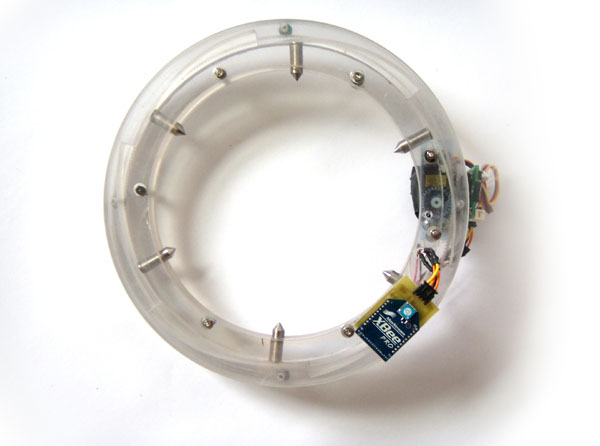
\includegraphics[height=2.5in]{thighmaster-alone}}
		\subfigure[As worn on leg]{\label{fig:thighmaster-leg}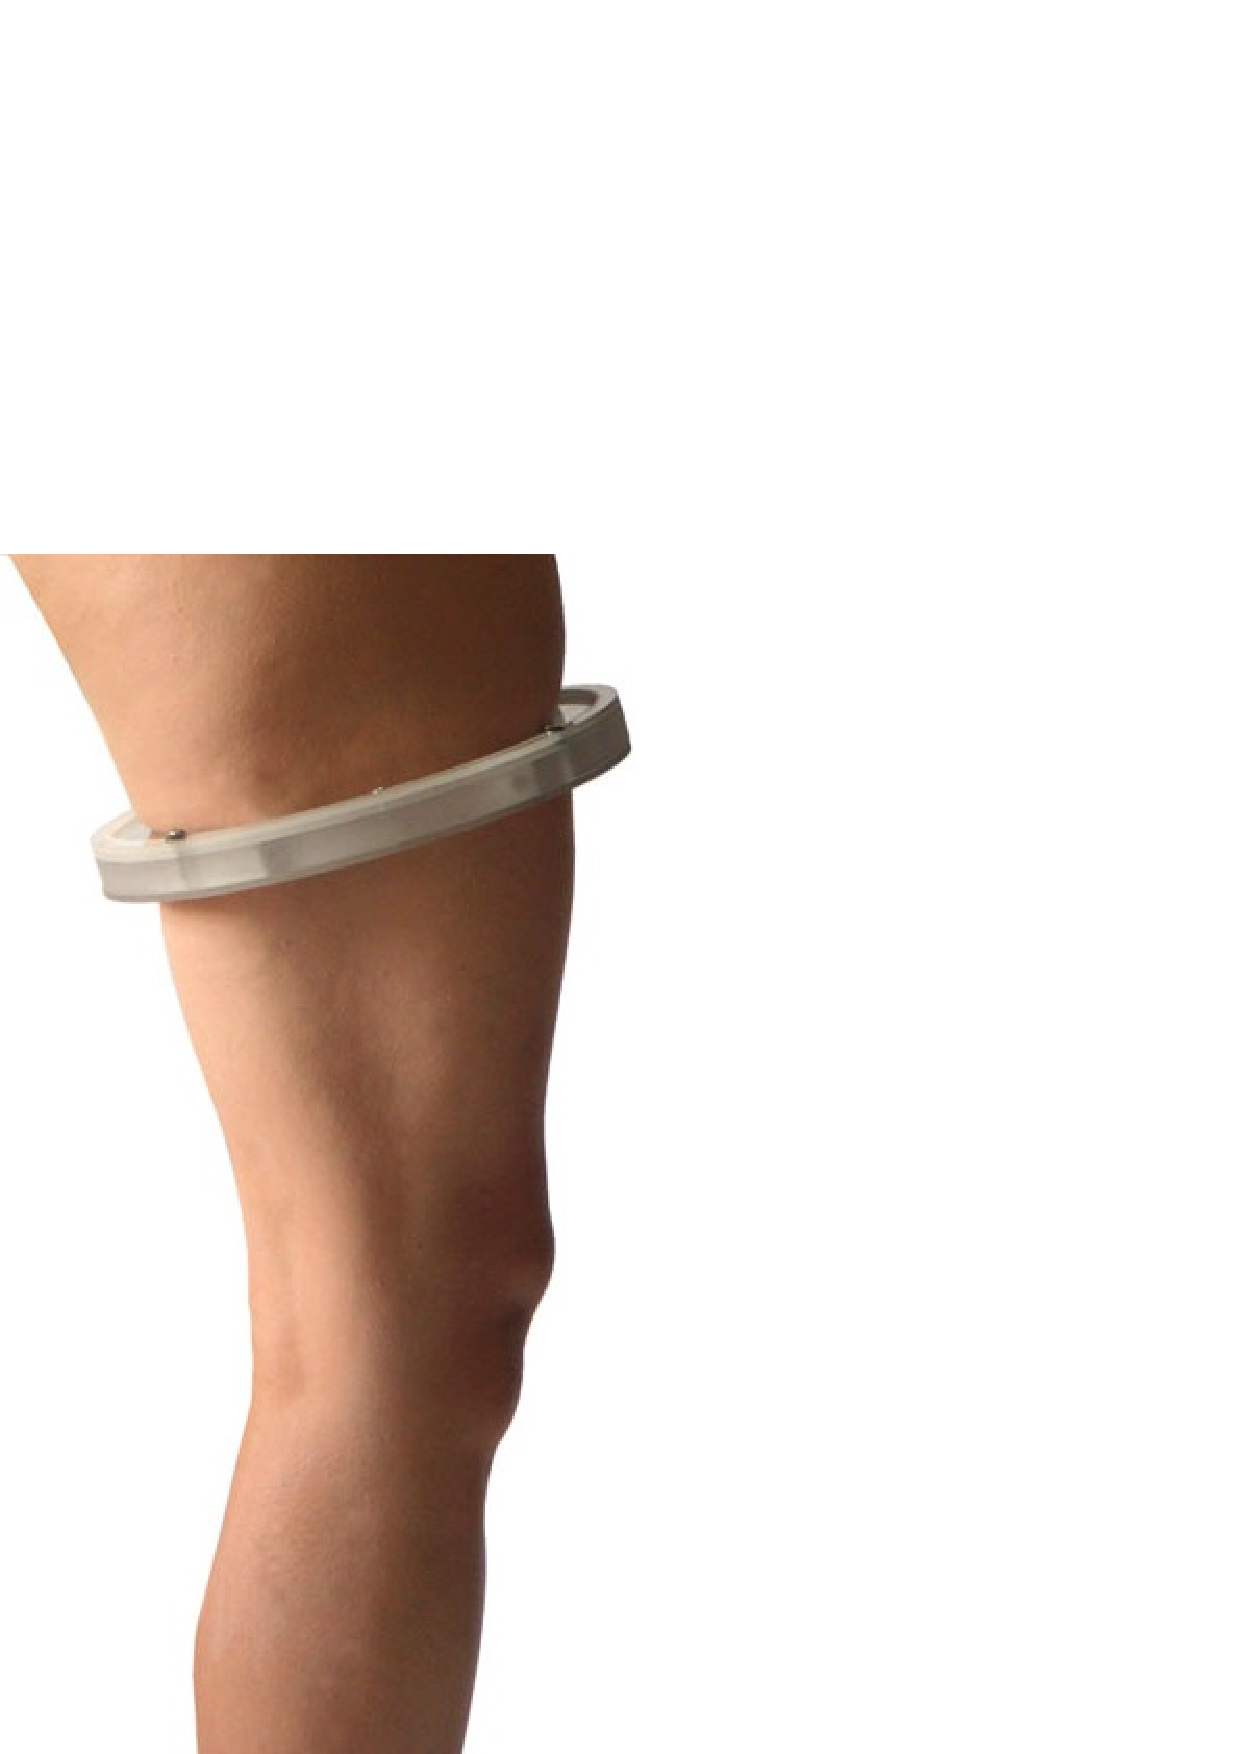
\includegraphics[height=2.5in]{thighmaster-leg}}
		\caption{Thighmaster energy feedback mortification device}
		\label{fig:thighmaster}
\end{figure}

R\"{u}st has implemented an extreme energy feedback system called the Thighmaster \cite{Rust2008Thighmaster-web}. Inspired by the cilice (a small metal garter with inward facing spikes) worn by some members of the Catholic Opus Dei organization as part of a practice of mortification, the Thighmaster is a ``techno-garter'' that pokes the wearer with spikes when their actions are not environmentally responsible (as defined by R\"{u}st), see \autoref{fig:thighmaster} for a depiction of the device. Specifically, the Thighmaster communicates wirelessly with electricity usage sensors and a human speech sensor that monitors whether the user speaks with their plants. While more of a demonstration, the Thighmaster shows the complex emotions involved in people's reactions to climate change. It goes without saying that being pierced by spikes is unlikely to be a viable energy feedback mechanism for most users.


\section{Related Systems}
\label{sec:related-systems}

In this section we examine other systems that have been designed to help users become more aware of their environmental impact, or make environmentally-positive behavior changes.

In a position paper, Sutaria and Deshmukh describe using networks of ad hoc sensors to monitor both electricity usage and miles driven by automobile, while providing real-time feedback to the user \cite{sutaria-2008}. The system described would compare the household's energy usage with others in similar situations. They envision smart energy meters that can also provide suggestions on how users can reduce their energy usage. They also mention the possibility of integrating personal carbon trading (a sort of carbon cap-and-trade system for individuals) into the system. The system described by Sutaria and Deshmukh appears to be hypothetical at this point.

\subsection{StepGreen}
\label{sec:stepgreen}

StepGreen is a web application designed to encourage people to undertake environmentally responsible actions \cite{step-green-website}. Mankoff et al.\ have written about the rationale for the system and description of the design, presumably written before the site was active \cite{Mankoff2007Leveraging-Soci} \fxnote{Should update with more recent StepGreen paper(s)}. The paper introduces the fact that, in the U.S., half of a person's energy consumption is their control. Therefore, by modifying their behaviors, Americans can affect up to half their \COtwo emissions. StepGreen (also known as Footsteps, possibly an earlier name for the system) is designed to leverage online social networks to motivate personal change, by providing suggestions for improvement.

\begin{figure}[htbp]
	\centering
		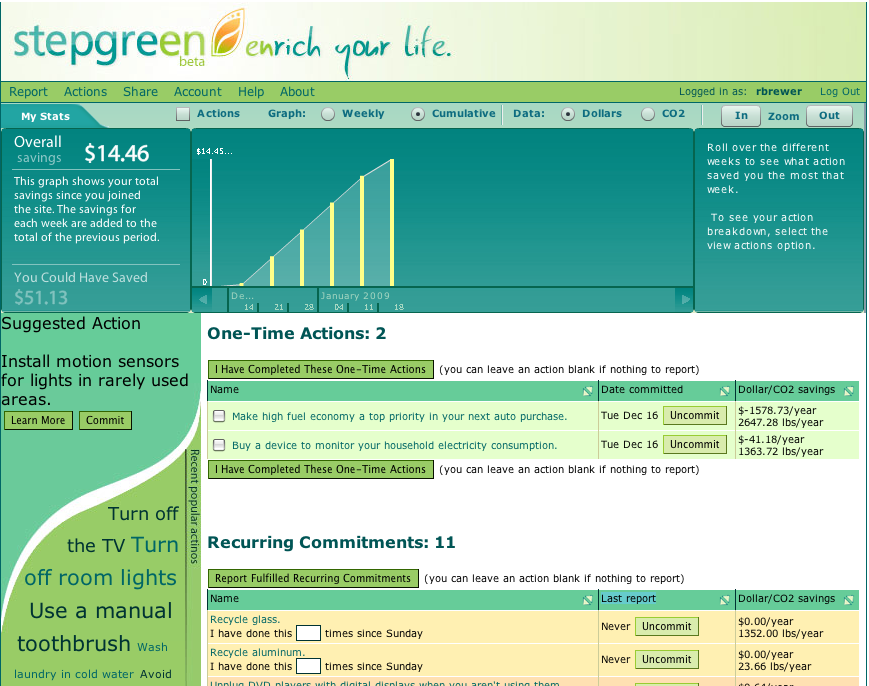
\includegraphics[width=\textwidth]{stepgreen-bitmap}
		\caption{Example page from StepGreen website}
		\label{fig:stepgreen-website}
\end{figure}

The StepGreen system is currently open to the public. \autoref{fig:stepgreen-website} shows an example of the default page shown when a user logs in. Users create an account on StepGreen, and then are presented with a list of actions with positive environmental consequences (mostly reduced GHG emissions). Example actions are ``Turn off the lights when you exit the house in the morning for the day'', ``Take the stairs at work'', and ``Set your home computer to automatically hibernate/sleep after a short period of inactivity''. Each action is associated with its cost savings and reduction in \COtwo emissions. Users can get more information about the action and how the savings were calculated. For each action, users can indicate whether they are already performing that action, whether they commit to undertaking that action, or whether the action is not applicable to them. Users can create new actions to be added to the list, but since the new actions have not been analyzed by the site maintainers, the financial and \COtwo savings are listed as unknown.

Once users have selected actions that they are either already performing or commit to performing, they can track them on the Reporting page. For one time actions, such as replacing an incandescent light bulb with a compact florescent bulb, users simply check off when they are completed. For recurring actions, users must indicate how many times they have performed the action since their last report in order for the system to track the activities. Based on the user's self-reporting, StepGreen calculates the amount of money saved, pounds of \COtwo saved (i.e., reduced), and missed pounds of \COtwo saved, and provides a historical graph of these values.

StepGreen also provides links to social networking sites. They provide a linked Facebook application, a MySpace profile widget, and a connection to Twitter. Each of these links provides a way to inform the user's social network about what actions the user is undertaking. This feature can serve to recruit other people to use StepGreen, provide comparisons on financial and environmental savings among peers, and encourage users to keep to their StepGreen commitments. 

StepGreen provides a useful platform for research on convincing users to change their behavior to reduce their carbon footprint. For example, a virtual polar bear was implemented to motivate users to reduce their carbon footprint (see \autoref{sec:virtual-polar-bear}). Notes on the StepGreen research website \cite{stepgreen-research-website} indicate that there are plans to support the input of sensor data from the UbiGreen transportation sensing project that they are a part of \cite{ubigreen-website}.

In its current state, StepGreen would be challenging to keep up to date due to the reliance on manual data input. Due to the limitations of manual reporting, StepGreen may report missed savings that are not accurate, annoying users. For example, recycling glass is an action that is listed as having substantial carbon savings. However, if one chooses to drink water from a mug instead of purchasing a beverage and later recycling the glass container, clearly the carbon savings are greater from using the mug, but StepGreen will count the lack of recycling as missed savings.

\subsection{Personal Kyoto}
\label{sec:personal-kyoto}

Personal Kyoto is a web service that tracks the electricity usage of users in the New York area, and compares it to a ``Personal Kyoto Goal'' for the user \cite{Personal-Kyoto-website}. The Personal Kyoto Goal represents the limit of electricity usage that would apply to the user if the Kyoto Protocol (which the USA is not a party to) were administered on an individual basis rather than on a national basis.

The user's electricity usage is retrieved from the local utility's web site (Con Edison) using the user's account number. In addition to the monthly usage (which can vary substantially due to circumstances and the seasons), a 12 month rolling average is computed to remove the seasonal effects. The Personal Kyoto Goal is defined as 75\% of the first point of the monthly rolling average when the user signed up with the web site. \autoref{fig:personal-kyoto} shows an example graph with monthly averages and a personal Kyoto goal.

\begin{figure}[htbp]
	\centering
		\includegraphics[width=\textwidth]{personal-kyoto}
		\caption{Example graph of electricity usage from Personal Kyoto}
		\label{fig:personal-kyoto}
\end{figure}

Personal Kyoto is a cleverly designed system in that it uses the user's real data, but avoids manual data entry by scraping the data from the utility web site. It also gives the user a specific goal for reducing electricity use that has a real justification and ties into the environmental ``gravitas'' of the Kyoto Protocol.

\subsection{EcoIsland}
\label{sec:ecoisland}

Takayama and Lehdonvirta have constructed a system they call EcoIsland, which attempts to ``motivate behaviour changes that reduce CO2 emissions'' using a background game-like activity, with a centrally installed display in the home \cite{takayama-2008}. \autoref{fig:ecoisland} shows an example of the user interface. Each family member has an avatar on the virtual island, and they set a family \COtwo emissions target. The family's emissions are tracked via sensors and self-reporting. If the emissions exceed the chosen target level, the water level on the island rises, and if the water level continues to rise it will eventually end the game.

\begin{figure}[htb]
	\centering
		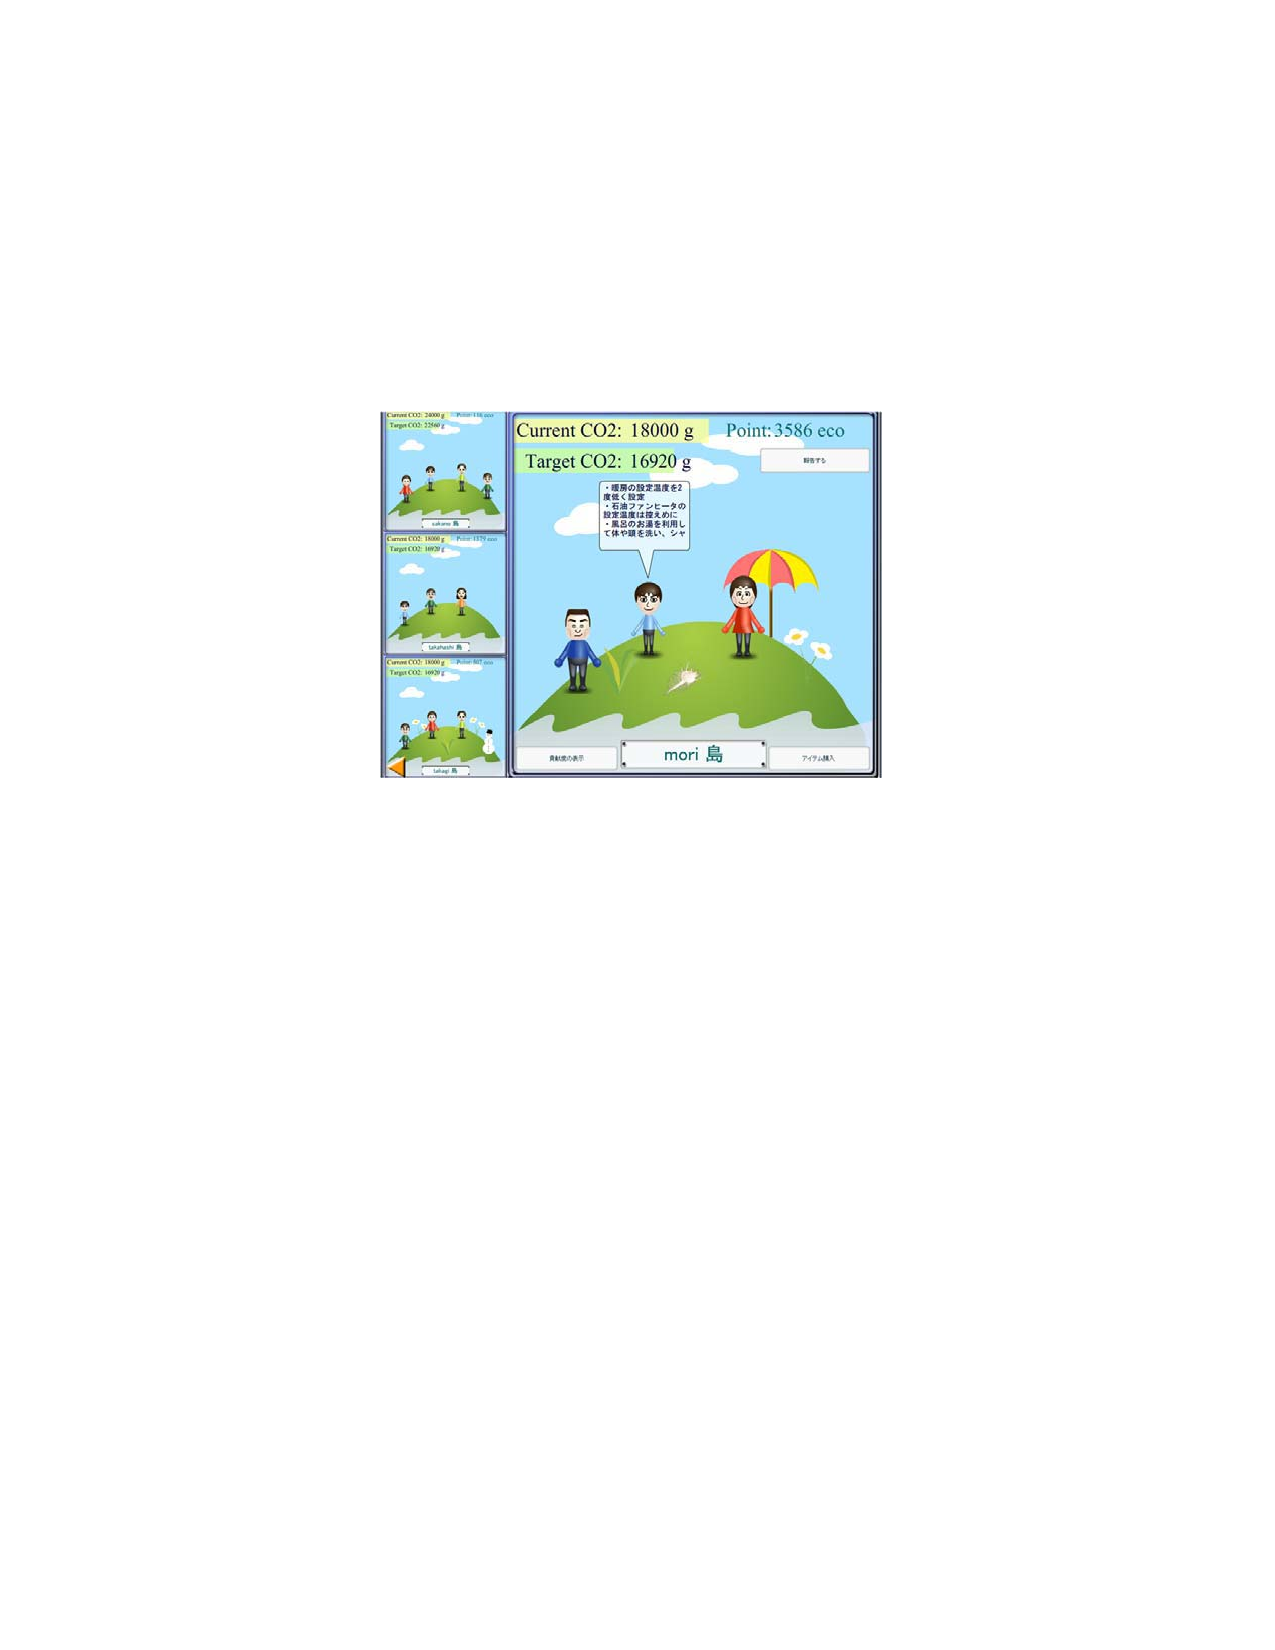
\includegraphics[width=0.8\textwidth]{ecoisland}
		\caption{Example EcoIsland display, with family avatars}
		\label{fig:ecoisland}
\end{figure}

Participants mobile phones have a list of suggested actions to reduce emissions, and they can self-report their actions using the phone. Participants can see the islands of other participants and they receive a periodic allowance in a virtual currency. The participants can use the virtual currency to buy decorations for their island, or to purchase carbon credits from other users. Participants with low emissions, therefore, can decorate their island, while those with high emissions have to spend their money on carbon credits. EcoIsland provides a metaphor for the users' emissions and makes them aware of the consequences of their actions.

The sensor portion of the system was not yet implemented at the time the authors conducted their study. The authors performed a four week pilot study of EcoIsland with 20 people in six families. During the first week, the baseline electricity usage of each participant's air conditioning system was monitored using a plug load meter (for more information on this type of meter, see \autoref{sec:plug-load-meters}). During the second week, one participant from each household was asked to use the system, while in the third week all members were asked to use it. In the fourth week, the carbon trading system was introduced to participants. At the conclusion of the study, the participants were surveyed and 17 of 20 participants said ``they were more conscious of environmental issues after the experiment than before.'' However, users indicated that they were motivated by game issues (such as saving the sinking island and buying in-game decorations) rather than saving the environment. Few of the participants used the carbon trading system because their targets were easy enough to achieve without trading. Air conditioner usage in participant homes showed no correlation with game outcome, but the authors believe that the short study may have affected that outcome. The study was conducted in winter, which might seem like an inappropriate time to measure air conditioner use. However, in Japan, many air conditioning units also function as heaters, so it may be this type of air conditioner usage that the authors are referring to. One interesting result is that participants noted that manual reporting contributed to their motivation, so replacing the reporting with sensors could reduce user's motivation to change.

\subsection{Google PowerMeter}
\label{sec:google-powermeter}

Utilities are starting to install `smart meters' (also called AMI for Advanced Metering Infrastructure) on homes as part of an overall push towards the `smart grid'. However, these smart meters are often thought about from the utility's perspective: eliminating manual meter reading, enabling time-of-day electricity pricing, and monitoring power reliability. While there are many benefits for the utility, frequently updated power data from the meter could be very useful if provided directly to the people being metered, as discussed in \autoref{sec:energy-feedback}.

Google PowerMeter is a web application developed to make smart meter data available to the end users living in smart metered homes \cite{Google-PowerMeter}. Google partners with utilities that have rolled out smart meters, and collects the power data from the utility. PowerMeter also works with the TED 5000 home energy meter that can be installed by end-users without interaction with the utility (see \autoref{sec:whole-home-meters}). The data is recorded at 15 minute intervals, and presented in a variety of graphs that show daily usage and home base load levels. \autoref{fig:google-powermeter} shows an example display for a home in \Hawaii. The primary interface for PowerMeter is a web gadget that is installed on the user's iGoogle home page. PowerMeter allows users to share their data with others, and has added an API to allow users to get access to their raw data.

\begin{figure}[htbp]
	\centering
		\includegraphics[width=\textwidth]{google-powermeter}
		\caption{Google PowerMeter data for a home in \Hawaii}
		\label{fig:google-powermeter}
\end{figure}

%\subsection{Microsoft Hohm}

\subsection{Virtual Polar Bear}
\label{sec:virtual-polar-bear}

Dillahunt et al.\ (who are involved with the StepGreen project) have built a system providing a virtual polar bear that is affected by the user's environmental choices as a means to motivate users to reduce their carbon footprint \cite{dillahunt-virtual-polar-bear-2008}. They note that there are strong emotional bonds between humans and animals, which may help to encourage environmentally-responsible behavior. The authors performed a one week study, with subjects divided into two groups: an attachment group and a control group. The attachment group read a story about climate change impacting polar bear habitats, and were asked to name their virtual polar bear. As participants make or decline commitments to environmentally responsible actions, the ice under polar bear either grows or shrinks (see \autoref{fig:virtual-polar-bear} for images of the polar bear). The study had 20 subjects (10 for each group), all of whom were surveyed before and after to test for levels of empathy and environmental concern. The subjects in the attachment group had more fulfilled environmental commitments, which was a statistically significant difference. The attachment subjects also had a greater level of environmental concern after interacting with the polar bear. The authors were unsure whether effects would be sustained in a longer study. They are now working on bringing the system to a mobile platform and creating a polar bear application for Facebook and MySpace.

\begin{figure}[htbp]
	\centering
		\includegraphics{virtual-polar-bear}
		\caption{Example images of virtual polar bear with lots of ice and with little ice}
		\label{fig:virtual-polar-bear}
\end{figure}

\subsection{iamgreen}
\label{sec:iamgreen}

iamgreen is an application for the Facebook social networking platform that provides an online gathering place for environmentally conscious users \cite{iamgreen-website}. iamgreen provides all of the standard components of Facebook: a newsfeed of events from members, status updates, news articles, etc. The application provides a list of environmentally responsible statements called ``leaves'', such as ``Most of my lightbulbs are compact fluorescents'', ``I recycle, even when it is not convenient'', and ``When I drive, it's over 40mpg baby'' (see \autoref{fig:iamgreen} for an example of the leaf selection page). For each statement, users can indicate if they engage in that behavior, they aspire to that behavior, they wish to hide the statement (removing it from the list of choices), or they want to recommend it to a friend. Users can then display the number of leaves they have committed to in their Facebook profiles. Users can also contribute new leaves, which will be displayed as options to other iamgreen users.

\begin{figure}[htbp]
	\centering
		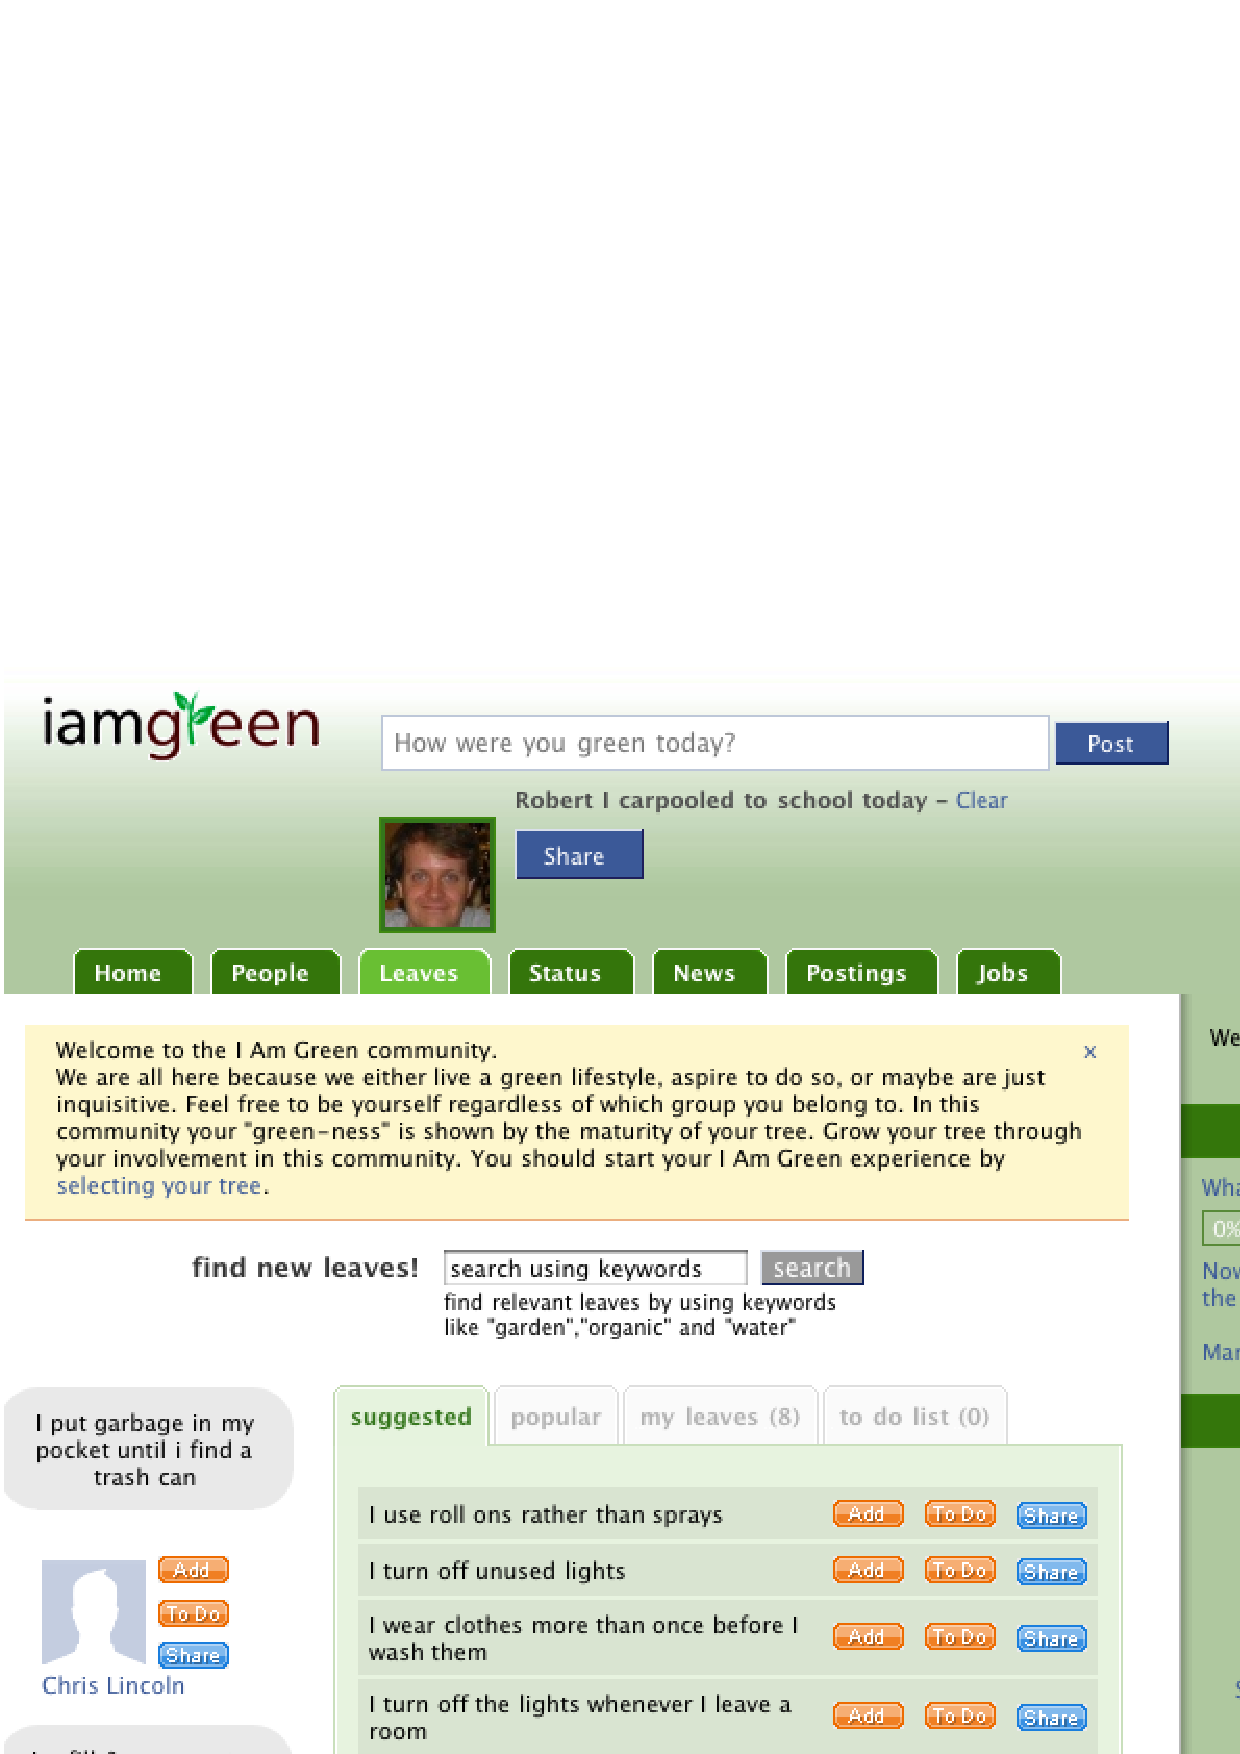
\includegraphics[width=0.8\textwidth]{iamgreen}
		\caption{Leaf selection page of iamgreen Facebook application}
		\label{fig:iamgreen}
\end{figure}

While the leaves concept is a simple way to encourage users to make more environmentally positive choices, it suffers from some obvious deficiencies. First, leaves, for the most part, have the same value (though apparently some actions, such as not owning a car, are worth more than one leaf). The leaf system also lacks any quantitative feedback other than the number of leaves, so the user is not provided with real insight into their environmental footprint. Like any system based on manual reporting, users have to spend time reporting any changes to their action list. Without quantitative feedback, it seems likely that many users will make some selection of leaves and then revisit them infrequently or never again.


\section{Motivation}

De Young investigated the motives behind individual's environmentally responsible behaviors (ERBs) through a series of surveys \cite{Young:2000fv}. Traditionally, the motives invoked by researchers attempting to promote ERB were constrained to material incentives or disincentives and altruistic reasons. The problem with incentives is that they ``needed constant reintroduction to remain effective and they proved to be less reliable than we had hoped''. Incentives can initiate ERB, but people's behavior changes back when the incentives end, and even continuing incentives can have low reliability.

De Young also describes some of the pitfalls that can be encountered in motivating ERB, such as psychological reactance, where people do the opposite of the ERB they are being asked to undertake. Even those initiating the behavior changes can be negatively impacted. De Young describes some initiators experiencing feelings of contempt for those whose behavior they are trying to change, and also contempt for themselves.

Self-interest is generally considered the cause of environmental problems: ``focusing solely on short-term individual or familial gain to the exclusion of long-term societal or environmental benefits''. De Young, however, suggests that self-interest can be a solution to environmental problems. He distinguishes self-interest from selfishness: self-interest meaning each individual is responsible for getting their own needs met. De Young believes that intrinsic satisfaction is a better way to motivate ERB, as people find that ``certain patterns of behavior are worth engaging in because of the personal, internal contentment that engaging in these behaviors provides.''

Based on 9 different studies of ERB across different populations and environmental focuses, De Young found 3 intrinsic satisfactions:
\begin{enumerate}
	\item ``satisfaction derived from striving for behavioral competence''
	\item ``frugal, thoughtful consumption''
	\item ``participation in maintaining a community''
\end{enumerate}

Competence involves the enjoyment in completing tasks and solving problems. Frugality is enjoyment from the ``careful stewardship of finite resources''. Participation is the enjoyment from participating in community activities such as sharing news and collaborating with others toward a shared goal.

While attitudes and norms can lead to behavior change, people also need tools and guidance to realize this change. As De Young puts it, ``without considering these variables, we make the error of assuming that once people know what they should do and why they should do it, they will automatically know how to proceed.'' In the particular case of competence as a motivator, it is important to provide people with the opportunity to utilize their competence or they will grow frustrated. He suggests that motivating through competence be accomplished by providing an environment where information on procedures is available and new behaviors can be tried out in a supportive environment.

Darby's survey of electricity feedback programs found similar results on motivations \cite{darby-review-2006}. She found that energy conservation efforts stopped when incentives were removed. When trying to get people to change their behavior, she found that behavior changes formed over a 3 month period is more likely to persist than changes made over shorter periods. She also found that internal motivation is most important for continued conservation efforts.

%In a position paper, Khan and Canny suggest that the technique of social marketing would be helpful in persuading users to make environmentally beneficial changes \cite{Khan2008-social-marketing}. Social marketing is the idea of applying the principles of consumer product marketing to encourage social change. The principles they describe are: emphasis on the benefits of new behavior while minimizing the cost, consumers are strongly influenced by knowing what behaviors others are undertaking. They suggest that target audiences be broken into different market segments, and each segment should receive messages appropriate to that segment. For example, in discussing the iamgreen application (see \autoref{sec:iamgreen}) where users commit to positive environmental actions suggested by others, the authors suggest using collaborative filtering (the technique used by online merchants to suggest other products similar to the one being viewed) to suggest the environmental actions presented to the user rather than just overall popularity of the actions.

\section{Fostering Sustainable Behavior}
\label{sec:fostering-behavior}

A variety of methods have been employed in an attempt to get people to change their behavior to be environmentally sustainable; McKenzie-Mohr provides a good summary of the area in his online book \cite{McKenzie-Mohr2009}. One of the most common techniques is the information-based campaign, which relies on providing information to the public through advertisements and documents like pamphlets and brochures. One type of information campaign attempts to shape peoples' attitudes towards an environmental issue, in the hope that those new attitudes will lead to more sustainable behavior. Unfortunately, these campaigns are usually unsuccessful. For example, Geller performed an investigation of the impact of three hour workshops on energy conservation that included a survey before and after the workshop \cite{Geller81}. The results of the survey indicated that the workshop had increased the energy literacy of the attendees and they indicated a willingness to implement energy conservation in their homes. However, followup visits with a selected group of 40 of the attendees found that very few had actually taken action (insulating their water heater or installing low-flow showerheads that had been given out during the workshops).

The other type of information-based campaign is based on financial incentives. In energy, this would include a utility advertising the rapid return on investment from a solar hot water heater, or promotion of rebates for more efficient appliances. This approach is also problematic, since it assumes that people are purely rational when making financial decisions, which they are not. For example, in 1983 California utilities were spending ``200 million dollars annually to promote energy conservation'' but with very limited success \cite{Costanzo86}.

To avoid the problems with information-based campaigns, McKenzie-Mohr has developed a process he calls Community-Based Social Marketing (CBSM) \cite{McKenzie-Mohr2009}. The process consists of several steps:

\begin{enumerate}
	\item identifying barriers to the desired behavior, and the benefits of the desired behavior to the individual
	\item developing a strategy to overcome the barriers using behavior change tools
	\item piloting the campaign on a small portion of the intended community, and making changes as needed
	\item evaluating the effectiveness of the campaign on fostering the desired behavior
\end{enumerate}

We focus here on the behavior change tools, which are critical to actually getting people to change their behavior: commitments, goals, and norms.

\subsection{Commitments}
\label{sec:rl-commitments}

Asking an individual to make a commitment has been shown to be an effective tool in changing behavior. In particular, an initial small, innocuous commitment can lead later to a larger commitment. For example, Freedman and Fraser conducted experiments in which subjects were asked to perform a small task (such as signing a petition to keep California beautiful) and then later asked to perform a more onerous task (such as placing a large billboard on their lawn that said ``Keep California Beautiful'') \cite{Freedman66}. They found that subjects that committed to the small task were much more likely to agree to the second task. The authors call this the ``foot-in-the-door'' technique. One of the reasons this technique is believed to work is the desire by individuals for self-consistency.

Making commitments public can increase their effectiveness. Pallak et al.\ studied residents that were asked to make a commitment to conserve electricity and natural gas \cite{Pallak80}. Some homes were asked to make a private commitment, while others were asked if their commitment could be publicized, though they were never actually published. Those that made commitments that they thought were public conserved more energy than the private committers, even one year later and after they were told that their names were not actually going to be publicized.

\subsection{Goals}
\label{sec:goals}

Goals can be thought of as commitments that can be objectively measured, which makes for a good pairing with feedback (see \autoref{sec:energy-feedback}). Becker investigated goal setting along with feedback of home electricity use \cite{Becker78}. Half of the subjects were given a goal of reducing electricity use by 20\% during the summer, the other half were given a goal of 2\%. The subjects given the higher goal conserved between 13\%--15\%, while the group with the smaller goal did no better than a control group. Houwelingen and van Raaij investigated use of natural gas in homes and compared daily feedback with monthly feedback and self reporting, with all groups having a conservation goal of 10\% \cite{Houwelingen89}. The group with daily feedback reduced their energy use by 12.3\%, and some reduction continued in the year after the feedback device was removed from their home.

\subsection{Norms}

Social norms are one way in which people's behavior is influenced by the behavior of others. Cialdini et al.\ make the distinction between descriptive norms (the way things are) and injunctive norms (the way things ought to be) \cite{Cialdini90}. In a series of experiments on littering, they found that subjects that the behavior of confederates of the researchers significantly changed the subjects' behavior. For example, subjects that viewed a confederate littering were more likely to litter a handbill that had been placed on their car. Also, subjects that viewed a confederate littering into a clean environment were less likely to litter than those that observed littering into an environment that already contained a lot of litter.

One problem with descriptive norms is that they can lead to `boomerang effects' where the norm has the effect of decreasing the desired behavior. Schultz et al.\ investigated this issue in the context of home energy conservation \cite{Schultz2007SocialNorms}. 290 homes were divided into two groups: one that would receive a written descriptive norm regarding their energy usage, and one that would receive the descriptive norm plus an injunctive norm. The descriptive norm showed subjects whether they were above or below the average energy usage in their neighborhood. The injunctive norm was simply a frowning or smiling emoticon based on whether the subject home was using more or less than the average consumption respectively. They found that homes that only received the descriptive norm led to energy conservation in homes above the average, but led to increased energy usage in homes below the average (the boomerang effect). However, those homes that also received the injunctive emoticon did not have a boomerang effect. Clearly injunctive norms are an important addition to any attempt to use comparative data to foster energy conservation.

Cultural norms can strongly influence what behaviors are non-negotiable. Strengers performed an ethnographic study of 10 households participating in a smart metering trial to examine how their comfort and cleanliness norms affected their energy savings \cite{strengers-comfort-norms-2008}. Participants were provided with metering devices that displayed electricity and water usage, and greenhouse gas emissions in real time. The author was attempting to use feedback to change the participants societal norms for comfort and cleanliness. For example, until relatively recently, bathing weekly was the norm, but now bathing daily is considered normal behavior. Like many people, the participants did not understand the connection between the consumption data and their practices. Participants tended to increase conservation by changing technology (such as using compact florescent lamps (CFLs) instead of incandescent light bulbs), or by minor behavioral changes like ``taking shorter showers, doing full loads of laundry''.

Strengers states that people act the way they do (in matters of cleanliness and comfort) because ``they believe society expects them to'' and because many companies and organizations have a vested interest in keeping it that way. Therefore, just providing people information about their consumption is not enough, because individuals are constrained by infrastructures and social norms. She suggests increasing social interaction regarding the feedback system by making placement more prominent and encouraging discussion with household visitors, because people tend to conform to the expectations of their peers.
However, it would seem that changing cultural norms is one of the hardest possible means for reducing consumption. It also feeds into many of the negative stereotypes of environmentalism: smelly people living in dark, cold homes. Despite the irrationality of some of these norms, effort may be better spent focusing on areas where the effort will meet less resistance.


\section{Design of Environmentally Persuasive Systems}

There is considerable research on the subject of designing environmentally persuasive systems. Woodruff et al.\ performed a qualitative study of individuals who are making a significant effort to be green, in an effort to inform future designs by documenting existing green practices and beliefs \cite{Woodruff2008-bright-green}. The participants were all involved in making their home more sustainable and energy efficient. The authors found that these environmentally inspired people have diverse affiliations. Traditional environmental activism, for example, isn't always central to their interests. Thirty-five homes participated in the study, with 56 people in total. The participants were mostly ``bright green environmentalists'', that is environmentalists that believe that technology can make the world more sustainable, rather than believing that technology is the root of unsustainable behavior and should be abandoned. The authors divided the participants into three groups based on their motivations: ``counterculture bio-centric activism; American frontier self-reliance and rugged independence; and trend-focused utopian optimism.'' The first group focused on stewardship of the earth, the second group on frugality, do-it-yourself activities, and patriotism from getting off foreign oil. The third group was focused on trend-setting, and being ``eco-chic''.

The authors found that the participants were reflective about the positive environmental choices they made, often trying to improve their sustainability through playful analysis of the options, such as buying a product online versus buying it from a store. They found that participants eagerly assessed the performance of their homes, so that they could tune their houses for better energy savings. This assessment included extensive data collection, both manual and automatic. In making their homes more efficient, the participants would work on improving one area at a time, then move on to the next area. However, after living in a house for 1.5 years, their interest in data collection had waned, in part because their routines had been internalized. Participants also wanted to live by example and inspire others, such as by driving a hybrid car.

Based on the interviews, the authors found several implications for design. The participants tended to learn about sustainability in a depth-based manner (focusing on one area at a time) rather than in a breath-based manner. Many popular attempts to encourage environmentally responsible behavior involve short lists of relatively easy actions, which is contrary to how the participants sought information. The authors suggest that advice systems focus on the user's primary motivations in an in-depth manner rather than providing a list of easy actions. The participants found mentorship to be an important part of the learning process, so the authors suggest that systems match mentees with mentors that have already mastered the area of expertise being sought. The authors suggest that users be provided with ways to express their identity and share their green activities to others via social networks. The authors observed that many participants enjoyed the process of determining the most sustainable option among many choices. Woodruff et al., therefore, suggest providing users with modest mental puzzles that help users explore the outcomes of different actions rather than telling them the answer outright.

Darby's review of energy feedback studies yielded some suggestions for design of environmentally persuasive systems \cite{darby-review-2006}. She observed that historical feedback of the user's energy consumption is more effective than feedback that compared usage to others, or feedback that compared usage to normative values. However, users did report finding pie charts of typical breakdowns of home energy use helpful, even though they were averages of all users rather than the user's own data. Although users reported that they liked to see comparative information, it didn't necessarily lead to energy conservation. In addition, if a user is shown comparative data that indicates that their usage is lower than their peers, it could lead to the user feeling less concerned about energy conservation.

Chetty et al.\ performed a qualitative study of the resource management processes of 15 households in an effort to help ubiquitous computing researchers design better resource feedback systems \cite{chetty-2008}. They found that participants were unaware of real-time resource consumption for both the entire home and individual appliances. The study examined the participants' usage of natural gas, electricity, and water. Thermostats were a problem for participants. They argued about how the thermostats should be set, and half of the homes with programmable thermostats hadn't actually programmed them. Some participants were in living situations where they paid a flat rate for their utilities, which led to a lack of motivation to conserve resources. Participants wanted real-time information on their resource usage, utility pricing (if there is peak load pricing), and also alerts if there is anomalous usage (such as a broken toilet using an excessive amount of water). The authors report that participants were also aware of potential privacy issues, such as being able to infer other's habits from their resource usage, and being able to detect the wasteful use of resources.

Based on their study, Chetty et al.\ provide some suggestions for future system designs. In the modern world, infrastructure is invisible: you don't have to know how much energy an appliance uses when you plug it in. Therefore, the authors suggest visualizations ``that equate our resource usage with units of production, for example, buckets of water, bags of coal, stacks of wood, as well as a monetary amount.'' They point out that households are often made up of multiple people with different levels of interest in being green and different responsibilities (some may not have to pay the bills!), so system design will have to reflect these differences. The authors also worry about the ``green divide'' in that lower income households might not be able to afford expensive equipment. They suggest the need to make sure devices supporting resource conservation are affordable to all.

One of the issues raised by Oberlin dormitory energy competitions is how to help residents sustain their interest in conservation principles and transfer their energy-saving behaviors once they leave the dormitory context \cite{Petersen09}. The dormitory energy competition is clearly able to reduce energy consumption when students are living in the dorms, but without engagement in larger issues (at the institution, community, or global level) then their long-term behavior may not be environmentally positive.


\section{Energy Literacy}
\label{sec:energy-literacy}

\emph{Energy literacy} is the understanding of energy concepts as they relate both on the individual level and on the national/global level. Solving the world energy crisis will require everyone to understand how energy is generated and consumed, so that they can make more informed choices in their lives and as informed citizens involved in their communities.

Defining and assessing energy literacy are therefore key to any attempt to improve energy literacy. DeWaters and Powers of Clarkson University have been working on an energy literacy survey instrument for middle and high school students \cite{DeWaters09c, DeWaters09}. They define energy literacy as consisting of three components: knowledge, attitudes, and behaviors. An example of energy knowledge would be understanding that the kilowatt-hour is the basic measure of electrical energy. Energy attitudes refers to concepts like needing to make more use of renewable energy in our power grid. Energy behaviors refer to specific things that can be done to reduce energy use, such as turning off lights when leaving a room.

Their survey consists of one section for each of the components, the knowledge questions using a multiple choice format, and the attitude and behavior questions using a 5-point Likert-style scale from strongly agree to strongly disagree. The pilot studies among 955 students showed students fared better on attitude (mean 73\%) and behavior (mean 66\%) scores, while mean knowledge scores were 42\%. DeWaters and Powers conclude from this that students may have the desired attitudes, but lack the knowledge to act on those attitudes.

Earlier work on assessing energy literacy includes a survey of attitude, knowledge, and intentions by Geller \cite{Geller81} given to participants at energy conservation workshops in the wake of the 1970s energy crisis.


\section{Electricity Metering}

Electricity metering systems can be broken down into two types: plug load meters that measure the electrical load directly plugged into them, and whole home energy meters that measure the electrical usage of an entire home. Both typically provide a real-time display of electricity usage, and some sort of historical total (usually in kilowatt hours, kWh).

\subsection{Plug Load Meters}
\label{sec:plug-load-meters}

The Kill-A-Watt is an example of an inexpensive plug load meter \cite{kill-a-watt}. It is designed to be plugged into a wall outlet, and the load is then plugged into the Kill-A-Watt. An LCD display shows the current voltage, current, power, frequency, power factor, and cumulative energy used since the unit was plugged in. The Kill-A-Watt provides an easy way to determine how much electricity a particular appliance (or set of appliances if connected via a power strip) uses. The manufacturer claims the Kill-A-Watt is accurate to within 0.2\%. There are several drawbacks to the Kill-A-Watt. Because of its shape, it generally obscures both of the outlets commonly found on a wall outlet in the US, preventing the second outlet from being use while measurement is taking place. The load must be plugged in via the Kill-A-Watt, so that means that the user must disconnect the load from power at least momentarily, which can be inconvenient for some loads (computers, refrigerators, etc.). The Kill-A-Watt also has no facility for exporting the data it collects, and if power is lost for any reason, the data collected will be lost as well. \fxnote{Add mention of newer model that stores data}

LeBlanc attempted to address the issue of data collection with his work on recording device-level power consumption \cite{leblanc-2007}. He developed a sensor that sits between the load and the wall outlet, like the Kill-A-Watt. The sensor records electricity usage, and transmits the data wirelessly using the ZigBee protocol to a base station. Details on how to construct the wireless power monitor can be found at the author's personal website \cite{LeBlanc2008power-mon-howto}. This system solves the problem of automated data collection, but still requires the load to be unplugged before monitoring. It also faces the problem of all plug-load meters, which is that it can only monitor what it is connected to, therefore it is unsuitable for providing a comprehensive picture of electricity usage in a home.

\fxnote{Need discussion of ACME meters here}

\subsection{Whole Home Meters}
\label{sec:whole-home-meters}

The Energy Detective TED Model 5000 is a whole home electricity meter from Energy, Inc \cite{the-energy-detective}. TED consists of three components:

\begin{itemize}
	\item a Measuring Transmitting Unit (MTU), which is connected directly to the incoming power lines at the circuit breaker box
	\item a Gateway that receives data from the MTU through the electrical wiring of the home, stores it, and makes the data available via HTTP using an Ethernet connection
	\item a handheld, wireless display unit that provides a continuously updated display of power usage sent via the Zigbee protocol from the Gateway.
\end{itemize}

The MTU uses current transformers, which clamp over the incoming power cables, and measure the amount of current being transmitted over them. Because the transformers clamp over the existing cables, there is no need to alter the existing wiring. The instantaneous power consumption can be computed using the current data combined with the utility voltage. These data are transmitted to the display unit through the home's electrical wiring.

The display unit receives the instant power consumption data from the Gateway unit every few seconds. The power consumption data can be displayed in real time in kW or dollars (after the user enters pricing data). It can also track historical consumption, peak usage, and project usage for the rest of the month based on historical usage. The Gateway unit provides a detailed web interface to the power data for computers inside the home, and can be configured to upload data to Google PowerMeter (\autoref{sec:google-powermeter}) every 15 minutes. Energy Inc makes an XML API available for developers who wish to use the data directly. TED appears to be the lowest cost option for whole home electricity monitoring with data recording and Internet accessibility.

While whole home energy meters provide only household-wide usage data, users can use the real-time display to figure out the impact of particular uses as air conditioning through trial and error experimentation. Parker et al.\ describe a protocol for using a household-wide meter and a circuit breaker panel to localize the energy usage in a home \cite{Parker2006How-Much-Energy}. All the breakers are turned off, and then turned on one at a time while recording data from the electrical meter. In 2--4 hours, users were able to generate a spreadsheet mapping the electricity usage in their homes.

\subsection{Building Energy Displays}
\label{sec:building-energy-displays}

Another type of electricity usage monitoring is building energy displays, which monitor electricity usage for an entire building (usually non-residential, such as a school or office building) and display the usage information in some public area such as a lobby. Green TouchScreen \cite{greentouchscreen} and Building Dashboard \cite{building-dashboard} are examples of this type of product. These devices aim to make building occupants aware of the overall environmental impact of the building, which is something usually invisible to the occupants. Some systems make the displays available via the web so that users can view the information from their desk as well as the lobby. The displays often provide  information beyond just electricity usage, such as water or natural gas usage, and may display the usage in units other than kWh, such as number of incandescent light bulbs lit or hours of TV watching. Beyond their potential utility in helping building occupants to reduce their energy usage, informative displays can be used to get points toward Leadership in Energy and Environmental Design (LEED) certification for a building.





% \section{Does Energy Efficiency Reduce Carbon Emissions?}
% \label{sec:efficiency-rebound}
% 
% Many governmental plans to reduce GHG emissions involve improving energy efficiency in the home, in industry, and in transportation. While intuitively it would seem that increased energy efficiency would lead to decreased energy usage, and thereby reduced GHG emissions, surprisingly there is some evidence (both theoretical and empirical) that energy efficiency actually increases energy usage! Saunders dubbed this unintuitive notion the Khazzoom-Brookes Postulate based on conclusions reached independently by those two researchers \cite{saunders-1992}. \fxnote{Insert references to Khazzoom and Lovins papers here, after I read them.}
% 
% Using neoclassical growth theory, Saunders finds that increased energy efficiency makes energy seem cheaper, thus allowing it to be substituted for labor in production. Increased energy efficiency also increases overall economic growth, which leads to increased overall energy usage.
% 
% In discussing this effect, rebound is defined as the difference between the expected amount of energy savings from an improvement in energy efficiency, and the actual observed effect. For example, if an improvement in metal smelting technology reduces the energy required to smelt by 20\%, but the energy consumed by the metal smelting industry only goes down by 10\% then the rebound is 50\%. If the rebound is greater than 100\%, then backfire is taking place (the efficiency measure has backfired) \cite{Hanley2008Do-increases-in}. There is some debate over whether the predicted increases in energy usage will actually take place in the real world. Laitner suggests via a simple analysis that the rebound effect is small (2.4\%) \cite{Skip-Laitner:2000yg}. His equation relates future carbon emissions to current carbon emissions, increases in GDP and energy costs, and elasticities of income and energy prices to arrive at this conclusion. He goes on to a further analysis done by the Environmental Protection Agency and Lawrence Berkeley National Labs using the National Energy Modeling System showing that an ``energy-efficient/low-carbon technology path'' would suffer from a rebound effect of only 2.2\%. However, he acknowledges that consumer choices about energy usage could erode gains from efficiency, such as turning up the furnace thermostat because the cost of doing so has been effectively reduced.
% 
% The issue of consumer choices is a real one. Over the last 25 years, automobiles have been made more efficient through ``increasing the efficiency of the engine and transmission, decreasing weight, improving tires and reducing drag'' \cite{Heywood2008Fueling-Our-Future}. However, these improvements have been traded for vehicles that are larger, heavier, and faster, which has led to only modest improvements in overall fuel efficiency. This is an example of how energy efficiency may not always lead to reduced GHG emissions without motivating automobile users (and manufacturers) to buy and make fuel efficient vehicles.
% 
% Other authors find that rebound and even backfire are the likely results of economy-wide improvements in energy efficiency. The analysis of Hanley et al. finds that backfire occurs when economy-wide improvements in energy efficiency are made \cite{Hanley2008Do-increases-in}. Their theoretical analysis finds that if energy demand is relatively price-elastic (demand increases when prices are low and decreases when prices are high), then backfire will occur. Empirical evidence of rebound and backfire are hard to come by because there are indirect system-wide effects due to the increased efficiency, and these indirect effects are difficult to measure. The authors created a Computable General Equilibrium (CGE) model of Scotland that simulates the economy and environmental impact based on the inputs and outputs of the system. Using this model, almost all scenarios eventually result in backfire. They note that since non-renewable energy sources use more energy in their production than renewable sources, increased energy efficiency lowers the cost of non-renewables compared to renewables, financially favoring the use of non-renewables. Efficiency in energy production is therefore associated with a decrease in the use of energy from renewable sources. The authors also urge caution when reviewing sustainability measures such as the ratio of Gross Domestic Product (GDP) to energy usage or carbon emissions, because even if the ratio increases (less carbon per unit GDP), if the GDP as a whole increases faster, the absolute carbon emitted will increase. They suggest that backfire could be prevented by combining energy efficiency improvements with taxes on energy use or a carbon tax. Since energy efficiency effectively reduces the cost of energy, the savings could offset the cost of additional taxes, thereby blunting any impact on economic activity.
% 
% It would appear that any energy efficiency improvements will have some degree of rebound effect, thus a naive pursuit of energy efficiency without taking into account the context around the improvements could risk reducing their effectiveness, or even making them counterproductive! While many of the analyses deal at the macroeconomic level, it is not hard to think of individual scenarios where efficiency could actually increase personal usage, such buying two energy efficient refrigerators to replace one older energy-hogging refrigerator. The key to ensuring that energy efficiency improvements on the micro level lead to less GHG emissions is to combine efficiencies with changes in behavior.

\chapter{System Description}
\label{cha:system-description}

This chapter describes the system I have evaluated as part of this research. By system, I mean all aspects of the 2011 Kukui Cup: the energy conservation competition, the point competition, the events that took place during the competition, and the underlying information infrastructure that supported it.

The 2011 Kukui Cup was designed with three goals in mind:

\begin{itemize}
	\item Enabling research into fostering sustainable environmental behavior change
	\item Improving the energy literacy of the participants
	\item Reducing the energy consumption of the residence halls
\end{itemize}

The participants competed both to reduce energy consumption in the participating residence halls, and to accumulate points by performing tasks related to energy literacy and conservation through the competition website.

\section{Setting}
\label{sec:setting}

The 2011 Kukui Cup took place in the Hale Aloha residence halls on the University of \Hawaii at \Manoa campus~\cite{hale-aloha-website}. Hale Aloha consists of four cylindrical towers, named after \Hawaiian flowers: Lehua, Ilima, Mokihana, and Lokelani. The towers are arranged around a central courtyard that contains benches, trees, and small raised platform that can be used as a stage. Next to the courtyard is a large cafeteria that provides meals for all the on-campus student residents.

The Hale Aloha towers were built in the 1970s. Each tower contains 13 floors with the following composition:

\begin{itemize}
	\item Floor 1: lobby (front desk, mailboxes, vending machine, TV)
	\item Floor 2: apartment for a Residence Director or Assistant Residence Director
	\item Floors 3--12: rooms for student residents
	\item Floor 13: laundry room, shared kitchen, meeting \& study spaces
\end{itemize}

The student resident floors (3--12) contain 14 inhabited rooms: 13 rooms intended for two residents, and one room designated for the floor's Resident Advisor (RA), who lives alone. There are two bathrooms per floor, each containing multiple individual rooms with a shower, toilet, and sink with a lockable door.

The even floors (4, 6, 8, 10, 12) have a sunken lounge space in the center of the floor with chairs, tables, and benches. The odd floors (3, 5, 7, 9, 11) share the lounge with the even floor above, accessed by a central stairwell. The pairs of floors are called ``lounges'' after their shared lounge space and labeled by letter: lounge A (3--4), lounge B (5--6), lounge C (7--8), lounge D (9--10), and lounge E (11--12). Hereafter, a lounge (pair of floors) will be specified using the name of the tower and the letter of the lounge, such as Ilima A or Lokelani C. With four towers, each containing five lounges, there are a total of 20 lounges participating in the competition.

There are two elevators in each tower: one that serves each floor (1--12), and one that goes only to the lounges (A--E and R, the roof lounge that is the 13th floor).

The residents' rooms include a pair of beds, armoires, desks, and chairs with one set arranged along each wall. In Lehua and Ilima, each side of the room has two power outlet boxes (4 outlets), while Mokihana and Lokelani have three power outlet boxes (6 outlets). Each room has two Ethernet jacks that provide Internet access. The student resident floors have have no central air conditioning, relying on windows for climate control (due to \Hawaii's climate, there is no need for heating). Residents with special needs (such as breathing problems or severe allergies) may request the installation of a room air conditioner at additional cost beyond the standard housing rates. There were three such air conditioning units approved during the Fall 2011 semester. Unapproved air conditioners are not allowed, and residents caught with one must pay a fine for energy consumption based on the number of weeks it was present in the room.


\section{Participants}
\label{sec:participants}

The participants of the competition were the residents of the four Hale Aloha towers. The residents were all first-year students starting at UH \Manoa. Each resident floor was overseen by a Resident Advisor (RA), a paid student employee who was in charge of enforcing rules, organizing activities, and being the first point of contact for residents. The RAs were allowed and encouraged to participate in and promote the competition.

These first-year student residence halls are specifically targeted for two reasons. First, based on conversations with UH \Manoa undergraduates, residents in the first-year residence halls are more likely to attend floor meetings and events, while upper-class residence halls are more like apartments where residents might not know their neighbors well or be motivated to attend floor meetings. Second, as the goal is to improve energy literacy and foster behavior changes in the participants, the earlier these changes take place in their college experience, the more benefit there will be to the participants and the University.

Each floor of the Hale Aloha towers has a resident advisor (RA) and 13 double occupancy rooms, and there are 10 floors of student residents per tower. Therefore at full occupancy, there are 270 potential participants per tower and 1080 potential participants in total.

The competition was run by a team of Kukui Cup staff, which included a professor, graduate and undergraduate students. The staff organized and ran events, put up marketing posters, and administered the competition website.


\section{Timing}

The 2011 Kukui Cup was organized into three rounds, each lasting a week. Two to three week student housing energy competitions are common (such as the one described by Petersen et al.~\cite{petersen-dorm-energy-reduction}), and provide a balance between sufficient time to get participants involved and waning interest in a longer competition. The intensive event schedule, need for fresh energy literacy content, and logistical overhead of running the competition also made a longer competition infeasible for this inaugural Kukui Cup.

As discussed in \autoref{sec:participants}, the Kukui Cup took place in first-year residence halls in an attempt to increase participation by students just starting in a new environment, and hopefully thereby more receptive to new experiences. For this same reason, we wanted to hold the competition in the Fall semester, in the first half of participants' first year. The Fall semester at UH \Manoa starts in late August (August 22 in 2011), and ends in mid-December (December 15 in 2011). We scheduled the competition in the middle of the semester for two reasons. First, at the beginning of the semester students are settling into their new environment and dealing with their classes. I also needed time to gather baseline data on electricity usage before the competition started, precluding an early semester start. Second, starting late in the semester is complicated by the Thanksgiving holiday (which took place during the week of November 22 in 2011), and the increasing workload as the semester winds down. The 2011 competition started at midnight on Sunday October 16, 2011 and ended at midnight on Sunday November 7, 2011.


\section{Energy Meters}

Monitoring the energy use by the residents is a core aspect of this research. This section covers the physical infrastructure needed to monitor energy use. Note that in the Hale Aloha towers, electricity is the only real source of energy in use (there is no natural gas or heating oil use). Therefore the energy monitoring is limited to monitoring of electricity use, and the terms energy and electricity are used interchangeably throughout this document.


\subsection{Meter Operation Principles}

Power meters typically work by sampling the voltage and current passing through a circuit to compute the power being consumed or produced ($Power = Currrent \times Voltage$). In a building setting, a meter will often measure the power being used by a single electrical distribution panel, which contains circuit breakers for the various loads in the vicinity. While voltages may be measured directly by connecting a voltmeter to one of the breakers, often the current present in home or institutional wiring are too large for convenient measurement by a meter. Current transformers (CTs) are used to step down this higher current to a more useable level. CTs are torus-shaped and typically have two pieces that can be clamped around existing wiring, allowing installation without breaking the existing electrical circuit. In an institutional setting, typically three-phase power will be used since it is a more economical use of conductor for heavy loads compared to single or two-phase power. To measure three-phase power, typically three ammeters (and thereby three CTs) and one voltmeter are required. A digital power meter will sample these four inputs at high frequency to compute power use, and also integrate over time to compute energy use (see \autoref{app:power-energy} for an explanation of the difference between power and energy).\fxnote{Add photo of meter and CTs}


\subsection{Meter Selection}
\label{sec:meter-selection}

The Kukui Cup energy competition required two out of the ordinary requirements for the energy metering: monitoring at the level of a floor as opposed to a whole building, and near real-time data collection at approximately 15 second intervals. In addition, we required that the meter provide a documented way to retrieve the energy data so that I could write software to collect and display the data.

Based on these requirements, we selected the Shark 200S meter from Electro Industries/Gauge Tech~\cite{shark-200s}. The Shark has an Ethernet port for Internet connectivity, and supports the standard Modbus TCP protocol~\cite{modbus-website} for queries of energy data. In addition to the Shark meter, three appropriately-sized CTs were needed for each meter to measure the current on the three phases of power present at each panel.


\subsection{Hale Aloha Electrical Infrastructure}
\label{sec:electrical-infrastructure}

I conducted a preliminary walkthrough of the Hale Aloha electrical infrastructure in August 2010. This walkthrough revealed there were two types of electrical distribution panels present on the resident floors:

\begin{itemize}
	\item A newly installed panel installed in the telecommunications room present on the even floors, which provides an additional power outlet box on each side of each resident room for the even floor and the odd floor below (ex. 3 and 4). I refer to these panels as ``telco'' panels, based on the label used outside of the telecommunications room.
  \item The original panel installed in the shared lounge area present between even and odd floors. These panels provide power to room outlets, overhead lights, and other circuits on the floors that share the lounge (ex. 3 and 4 for lounge A). I refer to these panels as ``lounge'' panels based on their location, however they monitor power use throughout the two floors, not just the small number of circuits used in the shared lounge space.
\end{itemize}

Energy meters like the Shark are designed to monitor the load from a single panel, by installing the CTs over the power lines coming into the panel. Attaching a meter to a telco panel will provide data on a segment of energy use for two floors (the new outlet boxes in resident rooms), but it is infeasible to break that down to a per-floor level. The lounge panels also monitor circuits spread across the two floors. However, the sum of the power use by the telco and lounge panels provides an accurate measure of the power use of the pair of floors that make up a lounge.


\subsection{Meter Installation}
\label{sec:meter-installation}

Getting the meters installed across the four towers proved quite challenging, despite the strong support of everyone involved, including UH \Manoa Student Housing. The Shark meters needed to be ordered through the university procurement process, and required installation by a externally contracted electrician. The telco meters were installed in the same room as the Ethernet switches that supply Internet connectivity to the floor, so those meters could be connected using a short cable. The lounge panels, however, had no nearby Ethernet jacks, so conduit and Ethernet cable had to be installed to connect back to the telco rooms.

Our efforts began in the summer of 2010, with the goal of running the inaugural competition in October 2010. However, the date was pushed back to February 2011 and then October 2011 due to delays in the meter installation process. \autoref{tab:meter-timeline} shows the timeline of when I first received valid data from a lounge (which requires both meters serving that lounge to be operating properly). The meters in Lehua were installed at the end of March 2011, while Mokihana and Ilima were not installed until September 2011. The meters in Lokelani were only installed shortly before the competition began in October 2011. Three meters experienced problems that made their data invalid after installation in Lokelani, and had to be replaced or adjusted. These failures further delayed the receipt of good data necessary for calculating baselines and running the competition.

\begin{table}[htbp]
	\centering
		\begin{tabular}{| l | c |}
			\hline
			Lounge & First valid data received \tabularnewline \hline \hline
			Lehua-A & 3/30/11 \\
			Lehua-C & 3/30/11 \\
			Lehua-D & 3/30/11 \\
			Lehua-E & 3/30/11 \\
			Lehua-B & 3/31/11 \\
			Ilima-A & 9/9/11 \\
			Ilima-B & 9/9/11 \\
			Ilima-C & 9/9/11 \\
			Ilima-D & 9/9/11 \\
			Ilima-E & 9/9/11 \\
			Mokihana-A & 9/9/11 \\
			Mokihana-B & 9/9/11 \\
			Mokihana-C & 9/9/11 \\
			Mokihana-D & 9/9/11 \\
			Mokihana-E & 9/9/11 \\
			Lokelani-A & 10/6/11 \\
			Lokelani-E & 10/6/11 \\
			Lokelani-D & 10/11/11 \\
			Lokelani-B & 10/14/11 \\ \hline
			\emph{Lokelani C} & \begin{tabular}[c]{@{}c@{}}1/23/2012\\\emph{(after competition)}\end{tabular}   \\ \hline
		\end{tabular}
	\caption{Timeline of meter installation}
\label{tab:meter-timeline}
\end{table}


\subsection{Energy Audit}

With the meters installed on both the telco and lounge panels, I was able to capture all the electricity use on the resident floors. However, one unknown is whether there were additional loads connected to those panels that were not under the control of the residents, and whether these additional loads were different between floors. Any differences could potentially throw off the results of the competition, and add uncertainty to any conclusions about resident behavior based on the energy usage data.

The original goal was to install all the energy meters during the summer 2011 break, when the towers are typically unoccupied. This would have allowed us to gather energy data with no residents present, which would have shown any hidden loads present on the floors. Unfortunately, all the meters were installed after residents were already present in the towers. The Lehua installation was completed at the end of March 2011, but Lehua was used to house summer session students, so it was never unoccupied long enough to complete an audit. Meters were installed in Ilima and Mokihana after the residents had moved in for the Fall 2011 semester, and the Lokelani installation was completed only shortly before the competition began.

To address this issue, a joint team from UH \Manoa Student Housing and the Kukui Cup project conducted an energy audit of the four Hale Aloha towers during the winter break after the Fall 2011 semester~\cite{csdl2-11-12}. Residents are not required to leave during the winter break, but many residents do leave, providing an opportunity to unplug all devices in resident rooms and examine the power usage recorded by the lounge meters. Other results from the energy audit can be found in \autoref{sec:post-energy-audit}.


\subsubsection{Panel audits}
\label{sec:panel-audits}

After each room was examined for devices to unplug, the overall power usage from each meter was recorded on a per-panel basis. \autoref{tab:power-per-panel} shows the power data that was collected.

\begin{table}[htbp]
	\centering
	\scriptsize
		\begin{tabular}{| l | c | c |}
			\hline
			Lounge & Panel & Power after unplugging (W) \tabularnewline \hline \hline
			Mokihana D & telco & 0 \tabularnewline \hline
			Lokelani D & telco & 3 \tabularnewline \hline
			Lehua B & telco & 4 \tabularnewline \hline
			Lokelani C & telco & 4 \tabularnewline \hline
			Lehua D & telco & 4.5 \tabularnewline \hline
			Lehua A & telco & 4.7 \tabularnewline \hline
			Lehua E & telco & 4.8 \tabularnewline \hline
			Ilima B & telco & 4.8 \tabularnewline \hline
			Lehua C & telco & 5.4 \tabularnewline \hline
			Lokelani E & telco & 5.7 \tabularnewline \hline
			Lokelani A & telco & 6 \tabularnewline \hline
			Ilima A & telco & 6.8 \tabularnewline \hline
			Mokihana A & telco & 6.8 \tabularnewline \hline
			Ilima D & telco & 7 \tabularnewline \hline
			Lokelani B & telco & 7 \tabularnewline \hline
			Mokihana B & telco & 7 \tabularnewline \hline
			Mokihana C & telco & 7 \tabularnewline \hline
			Ilima C & telco & 7.5 \tabularnewline \hline
			Mokihana E & telco &7.7 \tabularnewline \hline
			Ilima E & telco & 8 \tabularnewline \hline \hline
			Lehua B & lounge & 65 \tabularnewline \hline
			Lehua E & lounge & 78 \tabularnewline \hline
			Mokihana A & lounge & 106 \tabularnewline \hline
			Lokelani D & lounge & 129 \tabularnewline \hline
			Lehua D & lounge & 130 \tabularnewline \hline
			Ilima B & lounge & 133 \tabularnewline \hline \hline
			Ilima A & lounge & 183 \tabularnewline \hline
			Lokelani A & lounge & 195 \tabularnewline \hline
			Mokihana D & lounge & 225 \tabularnewline \hline
			Ilima C & lounge & 227 \tabularnewline \hline
			Ilima E & lounge & 229 \tabularnewline \hline
			Ilima D & lounge & 230 \tabularnewline \hline
			Lehua C & lounge & 243 \tabularnewline \hline
			Mokihana C & lounge & 252 \tabularnewline \hline
			Mokihana B & lounge & 253 \tabularnewline \hline
			Lokelani B & lounge & 287 \tabularnewline \hline
			Mokihana E & lounge & 335 \tabularnewline \hline
			Lehua A & lounge & 682 \tabularnewline \hline
			Lokelani E & lounge & 694 \tabularnewline \hline \hline
			\emph{Lokelani C} & \emph{lounge} & \emph{1834} \tabularnewline \hline
		\end{tabular}
	\caption{Power use per panel after unplugging in increasing order}
\label{tab:power-per-panel}
\end{table}

From \autoref{tab:power-per-panel}, one can see that for all the telco panels, the power measured was roughly the 5\W that our meters appear to consume. This confirms that the new panels in the telecom/IDF rooms only provide power to plug loads in resident rooms.

\label{par:lokelani-c}
One glaring problem is the power recorded from the Lokelani C lounge meter. The Lokelani C meter had been reporting much higher power usage than all other lounges, double the average lounge at peak. As part of the audit, all the circuit breakers were turned off, but the meter still registered approximately 1800\W!\@ On 1/23/2012 an electrician was brought in to troubleshoot the problem. The lounge panels have main feeds that come up from the basement, and each of these lines splits in two to power two lounge panels. The CTs on the Lokelani C panel had been incorrectly installed on the incoming power lines \emph{before} they split off to the panel, instead of after. Thus the meter was functioning properly, it was just metering both the Lokelani C panel load and the load from Lokelani D. This explains the data I observed from Lokelani C: usage roughly double other lounge panels. For these reasons, the energy data from Lokelani C collected before and during the competition must be considered invalid, and has been excluded from all analyses.

The networking equipment (router, switch, and occasionally power over Ethernet injectors) located in the telecom/IDF room of each lounge was sometimes different across towers and lounges. For example, the equipment in Lehua D's telecom room was recorded as 40\W, while Ilima E used 180\W.

The lounge panels are more complicated, since in addition to the resident room plugs and overhead lights, they control other loads. \autoref{tab:power-per-panel} shows that the lounge power can go as low as 65\W, or as high as 694\W.

Unfortunately, it was not possible in this audit to track down all the loads from the lounge panels for a few reasons. Most lounges had one or more residents present, and based on readings from the telco panels, residents did not always unplug all of their devices. They also were free to make use of the bathrooms during the audit, which contain overhead lights and power outlets. The inserts on the lounge panels that list what each breaker controls were mostly out of date or missing, making it difficult to tell whether the load on a breaker was from a resident room or something else. With the residents present and the time constraints of this audit, it was not possible to track down unexplained power from most breakers on the lounge panels.

The lounges from Lehua B to Ilima B in \autoref{tab:power-per-panel} show loads primarily from the networking equipment and the Shark meter, with a few scattered smaller loads (20--30\W). The rest of the lounges have increasing numbers of loads beyond the networking equipment, some quite sizeable (up to 200\W). It seems quite likely that some of these loads were residents that didn't unplug their devices, plugged them back in before the audit was complete, or devices that were missed during a sweep of the room. However, on the basis of this audit, I cannot rule out that there might be loads totaling as much as 640\W in a couple lounges. Also, since the audit was performed at a single time, if there are non-resident loads that are time based, they could have been missed by the audit.

While I cannot rule out some limited amount of hidden electrical load on a few lounges on the basis of this audit, it appears that there are no large, pervasive hidden electrical loads in the Hale Aloha resident floors. While differences in power usage were observed from networking equipment, these differences would impact the absolute energy use of a lounge, but not their change in use over time. Thus these differences could potentially change the outcome of the competition between lounges, but would not affect changes in electricity use for a particular lounge over time.


\subsubsection{Meter Accuracy}

For the audits of Lokelani and Mokihana I used a Conserve Insight plug load meter from Belkin~\cite{belkin-insight} to directly measure the power usage from each piece of network equipment in the telecom room. I then added these values together and compared the result with power recorded by the Shark meter using the circuit breaker audit method. The two values were always within 10\%, which is well within the expected accuracy of the Shark meter with such a small load. This provides some assurance that our meter installations are providing accurate data.


\section{Energy Data Collection}

The energy data recorded by the meters has to be retrieved in order to be useful. To provide a way to collect, display, and analyze the Kukui Cup energy data, I developed an Java-based open source system called WattDepot~\cite{csdl2-10-05}. WattDepot provides an ecosystem for energy data, from the collection of data from meters, to storing it in a repository, to displaying it in a variety of formats~\cite{WattDepot}.

The WattDepot architecture is broken into three kinds of services:

\begin{itemize}
\item WattDepot \emph{sensors}, a software process customized for a particular brand of energy meter. A sensor requests data from a meter according to the meter's protocol, then sends it to a WattDepot repository for storage.

\item WattDepot \emph{servers}, which implement a REST~\cite{REST} API for accepting energy data sent from sensors and providing this sensor data (or analyses based upon the data) to WattDepot clients.

\item WattDepot \emph{clients}, which request data from WattDepot servers and either display the data or analyses directly to users or provide the data to higher level energy services.
\end{itemize}

Data retrieved by sensors is associated with a \emph{source} when stored in the server. Each physical meter is typically a source, but sources can also virtual combinations of other sub-sources. For example, as discussed in \autoref{sec:electrical-infrastructure}, the electricity used by each lounge is provided by two different panels with separate meters. To view the total electricity use of the lounge, I created a virtual source with the two meters feeding that lounge as sub-sources.

Once the energy data has been stored in a WattDepot server, clients can query the server for the amount of energy used by a source between two arbitrary points in time. Since the sensor data is only retrieved periodically, in most cases the endpoints for an energy query will not match up precisely with the sensor data. To solve this problem, the WattDepot server will linearly interpolate between the two nearest sensor data values before returning data to a client.

To retrieve data from the Shark meters, I wrote a sensor that retrieves two values from the meter: the instantaneous power consumed and an energy counter that records how many watt-hours have flown through the meter since it was constructed. The meters were polled every 15 seconds before and during the competition, and the resulting sensor data was stored in a WattDepot server. Both the sensors and server were installed on a Apple Xserve system housed in our research lab. The client use of the energy data is discussed in \autoref{sec:energy-data-integration}.


\section{Competition Design}

The Kukui Cup competition was designed to meet multiple needs. In order to be effective, the competition needed to be interesting and engaging for the participants, or they would not be interested in participating. As a research project, the competition also had to support the needs of our experimental design and data collection. In some cases, these two needs were in conflict, and I note those decisions in this section and in \autoref{cha:experimental-design}.

The Kukui Cup consists of two different competitions: an energy conservation competition, and a point competition. This section explains the design of those two competitions, and other important game components.


\subsection{Rounds}

The 2011 Kukui Cup was structured into three week-long rounds:

\begin{itemize}
	\item Round 1: Monday October 17 to Sunday October 23
	\item Round 2: Monday October 24 to Sunday October 30
	\item Overall Round: Monday October 31 to Sunday November 6
\end{itemize}

Each round began at the start of the beginning day (12:00 AM) and ended at midnight on the end date. Each round had separate prizes, and rule changes typically took place at the start of a new round, such as the referral bonus (see \autoref{referral-bonus}). In Round 2, the points earned and energy used in Round 1 were set aside so that each player and lounge started at zero. The goal of this point/energy reset was to encourage residents that did not participate initially to start participating in a later round without undue disadvantage. In fact, since some activities could be performed in either Round 1 or Round 2, a player starting in Round 2 had an advantage in winning Round 2, as they could accrue all those points to their Round 2 total. In the Overall Round, the score and energy totals from Round 1 and Round 2 are combined, as well as any points earned in the Overall Round.


\subsection{Energy Competition}
\label{sec:energy-competition}

The 2011 Kukui Cup energy competition had a straightforward goal: the lounge that uses the least electrical energy in the round wins. As discussed in \autoref{sec:electrical-infrastructure}, monitoring energy at anything other than the lounge level was infeasible, making the lounge the fundamental unit of the energy competition.

Most other building energy competitions (such as the Oberlin competition discussed in \autoref{sec:dorm-energy-competitions}) do not use absolute energy use as the metric for success. Most competitions record energy data before the competition, and then average that data in some way to produce a \emph{baseline} of energy usage for the unit of competition (floor, building, etc). The metric of success is then defined as the team that reduced their energy use during the competition by the largest percentage compared to their baseline usage. As most competitions involve buildings of different sizes, construction dates, and occupancy levels, comparing to baseline usage is the only way to provide normalization between the teams.

An unfortunate side effect of using percent energy reduction compared to a baseline as the success metric is that accurately determining the baselines is critical for a fair competition. As discussed in \autoref{sec:baseline-computation}, determining an accurate baseline is challenging and potentially error prone. Also, using a baseline opens the possibility of a team artificially inflating their energy usage during the baseline collection period to make it easier for that team to win the competition. In another potential scenario one can imagine two teams before the competition starts: team A is very conscientious about energy use and has already taken many energy saving measures, while team B uses energy very wastefully and has taken no energy saving measures. Team A would find it difficult to achieve much reduction from their baseline energy use during the competition, while team B can take the all the easiest energy-saving measures and achieve substantial reductions compared to their high baseline.

Absolute energy makes sense as a success metric for the energy competition because all four of the Hale Aloha towers have very similar construction, and they are all close to full occupancy since the demand for on-campus housing outstrips supply. On the other hand, baselines were used for the Daily Energy Goal Game, described in \autoref{sec:energy-goal-game}.

Participants were able to track their lounge's performance in the energy competition through the scoreboard provided on the competition website, as shown in \autoref{fig:energy-scoreboard}.

\begin{figure}[htbp]
	\centering
		\includegraphics[scale=0.6]{round-1-energy-scoreboard}
		\caption{Round 1 energy scoreboard}
\label{fig:energy-scoreboard}
\end{figure}

We provided information to lounges on how to reduce their energy consumption through the activities and events available through the point competition.


\subsection{Point Competition}
\label{sec:point-competition}

In the point competition, individuals earned points by taking actions related to energy literacy or sustainability mediated through the competition website. The points earned by individuals were also aggregated by lounge, to produce a score for each lounge.

One of the goals of the competition was to improve the energy literacy of the participants. As discussed in \autoref{sec:energy-literacy}, I defined energy literacy as consisting of knowledge, skills, attitudes, and behaviors. While the knowledge component can be conveyed through information displayed on the competition website, the behaviors require the participants to engage in activities outside the website. Further, research in environmental psychology described in \autoref{sec:fostering-behavior} indicates that the incorporation of techniques like public commitments can increase the likelihood of sustainable behavior change.

To increase the energy literacy of the participants and to motivate their participation, the website provides a variety of actions that participants can take. These actions are divided into three categories:

\begin{itemize}
	\item \emph{Activities:} one-time, verifiable actions
	\item \emph{Commitments:} ongoing, non-verifiable behaviors
	\item \emph{Events:} events scheduled at a particular place and time
\end{itemize}

The complete list of actions defined for the competition can be found in \autoref{app:actions}, and a summary of the actions can be seen in \autoref{tab:action-summary}.

\begin{table}[htbp]
	\centering
		\begin{tabular}{| l | c |}
			\hline
			Action type & Number available \tabularnewline \hline \hline
			Activities & 62 \\
			Commitments & 21 \\
			Events & 24 \\ \hline
		\end{tabular}
	\caption{Summary of the actions available during the competition}
\label{tab:action-summary}
\end{table}

Actions can be either locked or unlocked. An unlocked action can be completed by a participant, while a locked action is completely inaccessible to participants until it is unlocked. Actions may be initially unlocked, while some actions may require other pre-requisite actions to be completed first. Actions may also be locked until a certain date. In the 2011 Kukui Cup, the available actions were divided roughly into thirds, and only the first third was available in Round 1, with the the second third available in Round 2, and then all actions were unlocked in the Overall Round.

When a participant successfully completes an action, they earn points. The points are intended to reflect the difficulty of the action. \autoref{tab:point-rubric} shows a summary of the different point levels and what type of action they correspond to.

\begin{table}[htbp]
	\centering
		\begin{tabular}{| c | l | c |}
			\hline
			Point value & Type of action & Time requirement \tabularnewline \hline \hline
			5 & Tweet something or complete a commitment & 1--2 min \\ \hline
			10 & Watch tutorial video, slightly more involved activities & 5 min \\ \hline
			20 & Attend an event & 1--2 hours \\ \hline
			30 & Priority events or activities & 10--60 min \\ \hline
			5--50 & Creative activities (e.g.\ writing a letter to editor) & multiple hours \\ \hline
		\end{tabular}
	\caption{Summary of the actions available during the competition}
\label{tab:point-rubric}
\end{table}


\subsubsection{Social Bonus}

As discussed in \autoref{sec:energy-competition}, participants must work together to win the energy competition. Provide an incentive for participants to work together, some actions in the point competition were assigned a \emph{social bonus}. The social bonus was worth 5 or 10 points, and was applied only to actions where two or more participants could reasonably complete the action together such as attending an event or making a commitment. To obtain the social bonus, a participant submits the email address of another participant with whom they completed the action. If the participant corresponding to the email address provided has completed the action, then the social bonus requester receives the bonus points. The social bonus does not require reciprocation: participant A can list participant B for the social bonus, and receives points even if participant B lists another participant or nobody at all for the social bonus. The social bonus is a deliberately simplistic indication of social interaction, since it reduces to the exchange of an email address. There is no verification that an action where the social bonus has been used was completed collaboratively. However, obtaining another's email address provides participants with an excuse to initiate contact regarding the competition, and we felt this was sufficient justification for any point inflation that might result.


\subsubsection{Activities}
\label{sec:activities}

Activities are the most common type of action available to participants. Activities are one-time actions that can be verified through the competition website. Example activities are:

\begin{itemize}
	\item Watch a short YouTube video about Power \& Energy
	\item Replace an incandescent bulb with a compact fluorescent (CFL)
	\item Perform an energy audit of the participant's room
	\item Write a letter to the editor on a Kukui Cup topic
\end{itemize}

Once the activity has been performed, the participant must verify the completion in order to receive points. Each activity uses one of these four methods of verification:

\begin{itemize}
	\item A short answer to a question randomly selected from a list
	\item An uploaded image (often a digital photo)
	\item A textual free response
	\item A textual free response paired with an uploaded image
\end{itemize}

In each case, the participant enters their verification information, which is sent to a competition administrator for review. The administrator either approves the submission, at which point the participant receives their points, or reject the submission with an informative message that explains why the submission was rejected. When a submission is rejected, the participant can try again, taking into account the administrator's reply. The review process happens asynchronously, so participants do not immediately know if their submission has been accepted. However, any submission does count as completing the action, so other actions that depend on the action submitted are unlocked.

For example, the video activities where the user watched a short video about an energy or sustainability topic used the short answer verification type. Each video had several verification questions, and to make it more difficult for participants to cheat by sharing answers, the question posed to each participant was selected randomly.

Other activities are difficult to verify with text only (such as changing out a incandescent bulb with a CFL). For these activities, participants can take a picture that provides some proof that they have completed the activity (such as holding both the incandescent bulb and the CFL).

The free response verification type was used for activities where output of the activity was text, such as the letter to the editor activity. Free response could also be used for activities where the result was a URL to a resource, such as a participant-created video.


\subsubsection{Commitments}
\label{sec:commitments}

Commitments are intentions to behave in a certain way in the future. The commitments in the Kukui Cup are intended to either improve participants energy literacy or reduce energy consumption, but for practical reasons cannot be verified through the website as activities are (see \autoref{sec:activities}). Example commitments are:

\begin{itemize}
	\item Turning off the lights when leaving a room
	\item Turning off/shutting down all appliances before going to sleep
	\item Using sunlight instead of electric lighting
\end{itemize}

While each of these commitments should reduce energy use, verifying compliance would require a massive network of embedded sensors throughout the towers, with a consequent massive invasion of participant privacy. The inability to verify that commitments are being met could lead participants to cheat and make commitments that they had no intention of meeting, just to earn points. We addressed this issue in two ways. First, commitments made by participants are public to all members of the same lounge. By making them public, we hope to encourage peers to point out commitments that have been made but are being violated. As discussed in \autoref{sec:rl-commitments}, public commitments have been shown to be more effective than private commitments, providing further reason to make commitments public. Second, each commitment is only worth 5 points (with a possible 5 point social bonus), each participant can only make five commitments at a time, and each commitment lasts for five days. Since the competition lasts 21 days, this caps the number of points that a participant can earn from commitments at 200 points, which is low enough that a cheating participant (who commits with no intention of acting on the commitment) would not unbalance the point competition.

When a participant has made a commitment, they can return to the competition website in five days to collect their points. The participant verifies their completion of the commitment by clicking on a button to affirm that they did live up to the commitment. While this self-verification still allows a participant to receive points without actually performing the commitment, it requires the participant to make a conscious decision to do so. Participants can repeat commitments after they expire, if they wish.


\subsubsection{Events}
\label{sec:events}

We held 24 events and excursions as part of the competition. Events were generally workshops, games, or parties held on the UH \Manoa campus, while excursions took place off-campus. Some examples of events are:

\begin{itemize}
	\item Kickoff party (held on evening of first day of competition)
	\item Energy scavenger hunt (looking for devices using specific amounts of power)
	\item Wind farm tour
\end{itemize}

Participants could view the list of upcoming events on the competition website, and could sign up to indicate their desire to attend. Signing up for an event earned participants 2 points instantly. To verify attendance, at each event a competition administrator handed out small printed slips of paper that contain an \emph{attendance code}. Each attendance code is unique to the event, and contains a random string of characters generated by the website in advance, such as {\tt windfarm-it397}. After the event is complete, participants that attended can enter the attendance code they received into the competition website. The website then verifies that the code is valid, has not already been used, and corresponds to the event in question. Unlike activity verification, if the code is valid, the participant is awarded points immediately upon submission. To encourage participants to only sign up for events they actually wanted to attend, participants that signed up for an event but failed to enter an attendance code (either because they did not attend the event or they forgot to enter the code) were penalized 4 points: reversing the 2 point signup bonus and subtracting a 2 point penalty.


\subsection{Daily Energy Goal Game}
\label{sec:energy-goal-game}

As described in \autoref{sec:goals}, setting goals for energy conservation has been shown to aid in conservation efforts. To help lounges reduce their energy use, we created the Daily Energy Goal Game, where each lounge attempts to use less energy each day than the goal amount. The goal was determined by computing a baseline of energy use for each lounge and subtracting a fixed percentage from each baseline. At the end of each day, if a lounge had met its energy goal, each participant on the floor with a non-zero score received 20 points.

The Daily Energy Goal Game had two additional benefits for the competition design. First, it provided a short-term energy goal that participants could work towards, shortening the feedback cycle. If a lounge failed to meet the goal one day, the participants could redouble their efforts and try again the next day. Second, it provided a further linking of the energy competition to the point competition.

To aid participants in meeting their daily goal, the competition website provided a visualization of progress towards the goal, shown in \autoref{fig:energy-goal-game}.

\begin{figure}[htbp]
	\centering
		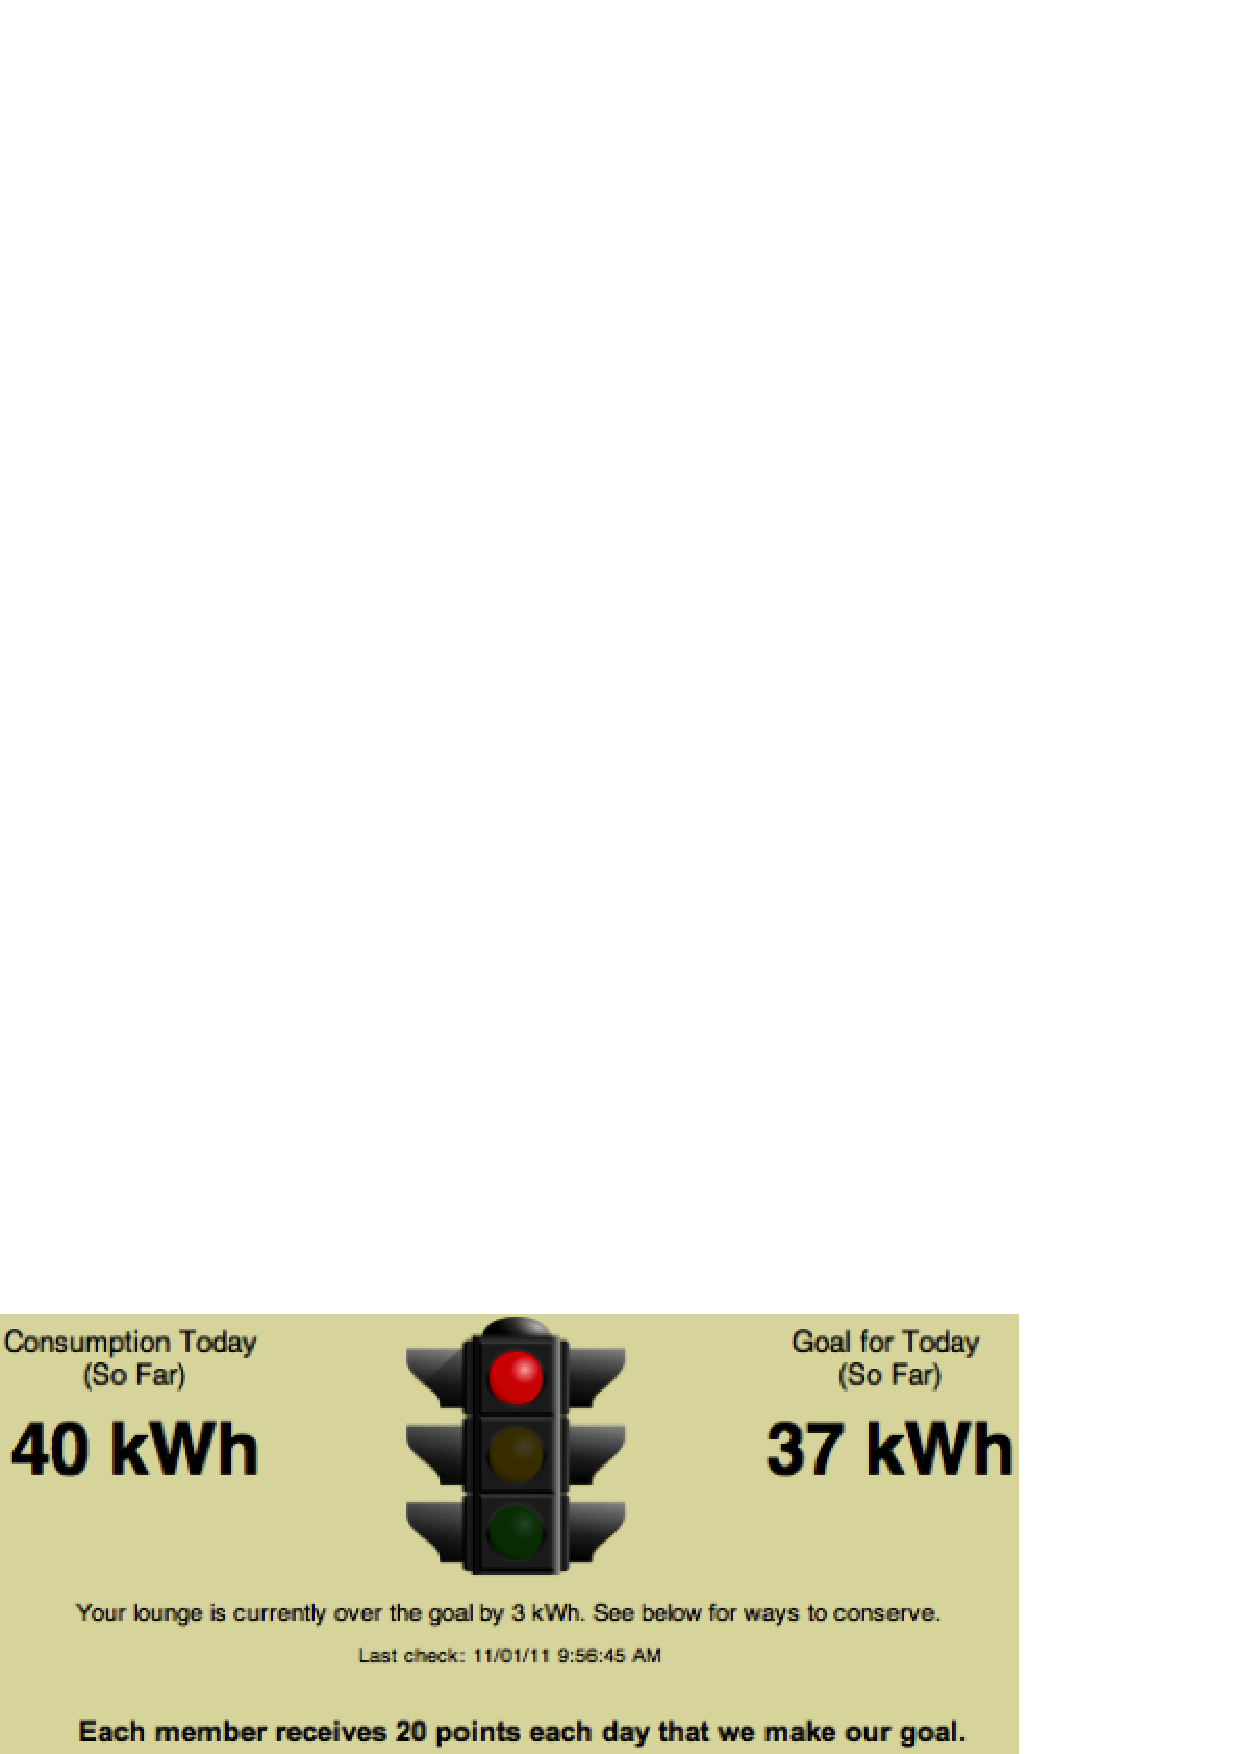
\includegraphics[scale=0.7]{energy-goal-game}
		\caption{Example of the Daily Energy Goal Game visualization}
\label{fig:energy-goal-game}
\end{figure}

We computed the baseline of each lounge's energy use on an hourly basis. The visualization shows the number of kilowatt-hours used by the lounge so far in the day, and compares it to the energy use goal. The traffic light indicates the energy use: red when the energy use is above the goal, yellow when energy use is just below the goal, and green when energy use is significantly below the goal. Both yellow and green thresholds are set by configuration.

It was important that the visualization compare the energy use for the day so far to an equivalent goal for the day so far. Since cumulative energy use is monotonically increasing, if the energy use was compared to the goal for the entire day, it would generally lead to a traffic light that is green for part of the day and then stays red for the rest of the day, which would not be an actionable visualization for participants. Further, we computed the baselines at an hourly granularity, which is important because energy use varies throughout the day. Computing a single daily baseline value and averaging it throughout the day would cause the visualization to show participants under the goal during the low usage period of the day, but then over the goal during the evening high use period.


\subsubsection{Baseline Computation}
\label{sec:baseline-computation}

The energy goal for the Daily Energy Goal game requires a baseline of energy use for each lounge. The baseline should reflect ``normal'' use, and be closely comparable to the energy use during the competition period. \autoref{fig:lounge-daily-power} shows the power used by one lounge over the course of a weekday before the competition, while \autoref{fig:lounge-weekly-power} shows the power used by the same lounge over an entire week. The energy use for the lounge differs from an average home or apartment in a few ways: the peak power usage is shifted to near midnight for weekdays, the lowest usage occurs between 8 AM and 10 AM which is typically a high usage period in homes. Usage also varies based on the day of the week: Friday and Saturday evenings have lower and earlier peaks compared to other nights. To capture these hourly and daily variations, we computed baselines each of the days of the week (seven daily baselines), and for each hour of each day of the week (168 hourly baselines).

\begin{figure}[htbp]
	\centering
		\includegraphics[width=\textwidth]{Ilima-B-daily-power}
		\caption{Example power usage by Ilima B for one day, pre-competition}
\label{fig:lounge-daily-power}
\end{figure}

\begin{figure}[htbp]
	\centering
		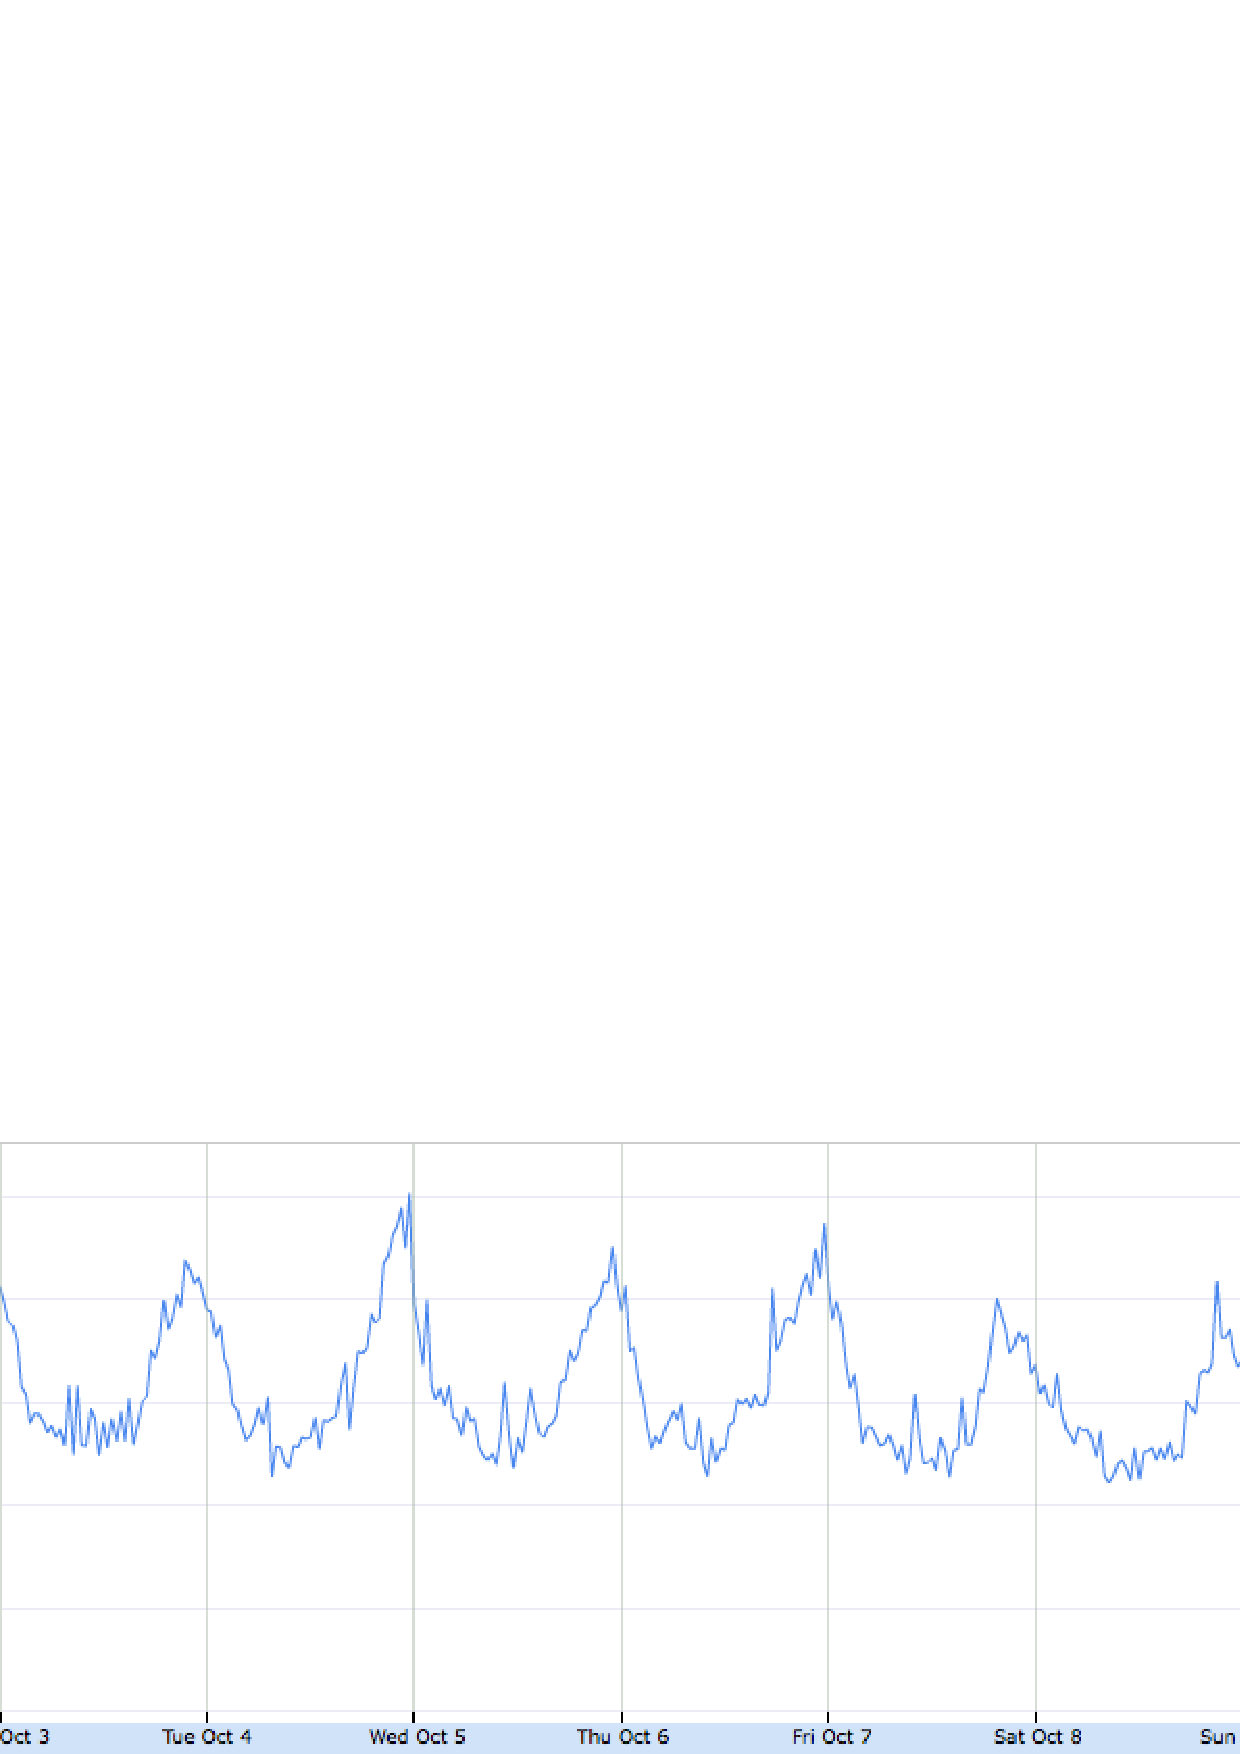
\includegraphics[width=\textwidth]{Ilima-B-weekly-power}
		\caption{Example power usage by Ilima B for one week, pre-competition}
		\fxnote{Replace with publication-quality graphs if time permits}
\label{fig:lounge-weekly-power}
\end{figure}

The competition ran for three weeks starting October 17, 2011. As shown in \autoref{tab:meter-timeline}, full days of meter data for all lounges were only available for Lehua, Ilima, and Mokihana starting on September 10. For lounges in these three towers, I computed the baseline as the average energy use from September 10 to October 15 (five full weeks plus one day). The delay in getting meters installed and working properly in Lokelani complicated the baseline computations for that tower. Lokelani A and E got their first full day of data on October 7, so the baseline was computed from October 7 to October 15 (one full week and two days). The baseline for the days of the week with two days of data are were averaged, the rest reflect the actual usage.

The late installation of the meters in Lokelani B, C, and D meant that I had less than one week of data for those lounges before the competition began. We felt that it was important from a competition perspective for all lounges to be able to participate fully in the competition, rather than exclude Lokelani B/C/D from participating in the the Daily Energy Goal Game or the entire competition. Lokelani C and D had data from Wednesday October 12 to Saturday October 15, so I used the actual usage as the baseline for those days of the week. For the remaining two weekdays (Monday and Tuesday), I computed the baseline by averaging the data from the three weekdays. Usage on Sunday is different from both weekday and Saturday usage, requiring some additional calculation to provide a reasonable estimate. I computed the ratio of energy use between Sunday and Saturday for each lounges in Lehua, Ilima, Mokihana, and Lokelani A and E. I found the average increase in daily energy use from Saturday to Sunday from the baseline period is 5\%, so the Sunday value for Lokelani C and D was the actual usage from Saturday October 15 multiplied by 1.05.

Lokelani B presented the biggest challenge in estimating an energy baseline, since I had only one full day of data from Saturday October 15. I assumed (for lack of other alternative) that the ratio of energy use between lounges on a single day is representative of the ratio of their energy use for each day of the week. For the weekday values, I computed the ratio of energy use on October 15 between Lokelani A and B, and between Lokelani B and E, since lounges A and E were in the same tower and had more than a full week of data. I set the baseline for each weekday as the average of the A to B ratio multiplied by the A  baseline for that day, and the B to E ratio multiplied by the E baseline for that day.\fxnote{Need series of plots showing energy use before competition, and then the 1 week baseline}


\subsection{Prizes}
\label{sec:prizes}

Prizes were awarded at the end of each round as incentives for participation. There were four types of prizes distributed:

\begin{itemize}
	\item The lounge that used the least energy (1 winner per round)
	\item The lounge with the highest score (1 winner per round)
	\item The individual with the highest score in each lounge (20 winners per round)
	\item The individual with the highest score across all lounges (1 winner per round)
\end{itemize}

In Round 1 and Round 2, only the score earned or energy consumed for that round was used to determine the winner, but in the Overall Round the overall score or energy was used. \autoref{tab:prizes} summarizes the prizes awarded during the competition. As one would expect, the prizes for the Overall Round were substantially higher value than the prizes for Rounds 1 and 2.

\begin{table}[htbp]
	\centering
		\begin{tabular}{| c | l | l |}
			\hline
			Round & Type of prize & Prize \tabularnewline \hline \hline
			1 & lounge energy & mochi ice cream party \\ \hline
			1 & lounge score & cupcake party \\ \hline
			1 & individual per lounge & \$5 ice cream gift certificate \\ \hline
			1 & individual overall & \$25 UH bookstore gift certificate \\ \hline
			2 & lounge energy & malasada party \\ \hline
			2 & lounge score & locally-made popsicle party \\ \hline
			2 & individual per lounge & \$5 gelato gift card \\ \hline
			2 & individual overall & \$25 UH food service gift card \\ \hline
			overall & lounge energy & pizza party \\ \hline
			overall & lounge score & pizza party \\ \hline
			overall & individual per lounge & \$10 UH bookstore gift card \\ \hline
			overall & individual overall & iPad 2 \\ \hline
		\end{tabular}
	\caption{Prizes awarded during competition}
\label{tab:prizes}
\end{table}


\subsection{Raffle Game}
\label{sec:raffle-game}

One problem with the prizes provided in the competition as incentives is that they only go to the top performers in each competition. For those participants that are aware that they will not win the point competitions, the prizes provide little incentive, or possibly a disincentive: why play if there is no way to win a prize? Another problem with the prizes is that to be effective they had to appeal to all participants, limiting the options for prizes.

We developed the Raffle Game to provide a prize-based incentive to play that was not limited to the top players, through inspiration from Balaji Prabhakar's work incentivizing road congestion reduction~\cite{Merugu2009}. In the Raffle Game, there are a variety of raffle prizes available in each round of the competition. For each 25 points a participant earns, they receive a virtual raffle ticket. Participants can allocate their raffle tickets among the prizes available, and they can change their allocations at any time. Shortly before the end of the round, the raffle is closed and the ticket allocations frozen. A winning ticket is ``drawn'' from those allocated to each raffle prize, and the owner of that ticket wins the prize. Tickets that are not allocated before the end of a round roll over to the next round, until the end of the competition. \autoref{fig:raffle-game} shows an example view of the Raffle Game for a user with many tickets, including the odds of winning.

\begin{figure}[htbp]
	\centering
		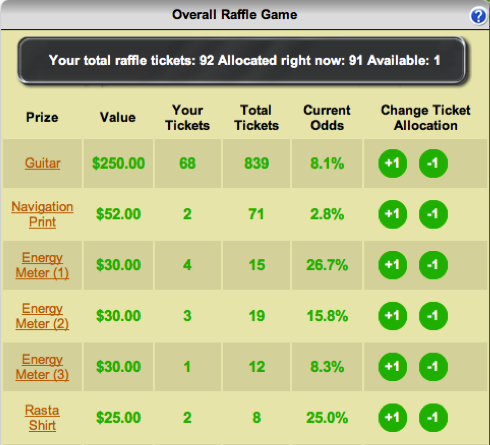
\includegraphics[scale=1.0]{raffle}
		\caption{Example display of the Raffle Game during Round 3}
\label{fig:raffle-game}
\end{figure}

The Raffle Game ensured that every participant that has earned at least 25 points in a round can have some slim chance of winning a prize. Participants can increase their odds of winning a prize by earning more points, providing a clear incentive for further participation. Since participants can choose which raffle prizes to allocate their tickets to, the prizes can appeal to diverse interests, unlike the competition prizes.

\section{Competition Website}

The Kukui Cup competition required extensive online support for both the virtual and real-world activities. We developed a custom web application called Makahiki to be the online focus for the competition. I was one of the principle designers of the functionality of the website, while application was implemented by George Lee, Yongwen Xu, with assistance from Greg Burgess, Nathan Dorman, and Nathaniel Ashe. The application is written in Python, using the Django web application framework~\cite{django-website}.

\subsection{Website Development}

The website was developed in an iterative fashion. An initial version was developed in Fall 2010 with limited input from anyone outside the development team. After showing this alpha version of the website to some external individuals, we received feedback that the website was too confusing and not sufficiently engaging.

Our next step was to develop a series of user scenarios, and visualize them using mockup web pages developed with Balsamiq Mockups tool~\cite{balsamiq-website}. The mockups were evaluated by a series of walkthroughs conducted with three UHM ICS faculty members, two community members, and two undergraduate students. Each evaluation was conducted using a think aloud protocol, as the subjects viewed each mockup screen on a projector, while the experimenter walked through each user scenario. We recorded the discussion between the subject and experimenter, as well as the computer display. After the evaluations, we revised the mockups based on the feedback we had received.

In Spring 2011, Makahiki was implemented using the revised mockups as the template. In April 2011, we conducted a series of in-lab user evaluations of the website using five first-year students who were living in the Hale Aloha towers. We told the subjects that the website they were evaluating was part of an energy competition we were going to hold in the Fall 2011, but no additional details, since one important goal of the competition website was to be self-explanatory. In the first part of the evaluation session, each subject was asked to pretend they were participating in the competition, using a think aloud protocol. Subjects interactions with the website were recorded as a screencast, along with audio from their interactions with the experimenter. In the second part of the evaluation, the experimenter went over parts of the website with the subject, while asking them questions about their experiences. After reviewing the comments from all five subjects, we generated a list of improvements to be made to Makahiki.

In July 2011, once the problems identified with Makahiki from the April evaluation had been resolved, we conducted another round of in-lab user evaluations with five more subjects. This evaluation was conducted in similar fashion, with participants pretending to be participants in the competition and using the website while their actions and discussion was recorded. These evaluations resulted in another set of improvements in Makahiki.

While the in-lab evaluations were helpful, each one involved less than one hour of play, and the website designers were at hand to answer any questions in person. The since we conducted the in-lab evaluations individually, they also didn't provide any insight into the competitive aspects of the Kukui Cup. To address this gap in our evaluation, we organized a beta test of the Kukui Cup in August 2011. We recruited four teams of five players, from friends, family, colleagues from industry, and local environmental organizations. The beta test consisted of two three day rounds to allow us to test the awarding prizes and the Raffle Game. The beta test uncovered several implementation defects that were corrected, as well as suggestions for additional actions.


\subsection{Website Functionality}

We designed the competition website to be as easy as possible for residents to start participating. This section describes the features of the website.


\subsubsection{First Login Process}

During the competition, when users went to the website~\cite{kukuicup-website}, they saw a landing page like the one shown in \autoref{fig:landing-page}. The landing page guides the residents eligible to play (those living in Hale Aloha) into the competition site, while providing some background information on the competition for everyone else.

\begin{figure}[htbp]
	\centering
		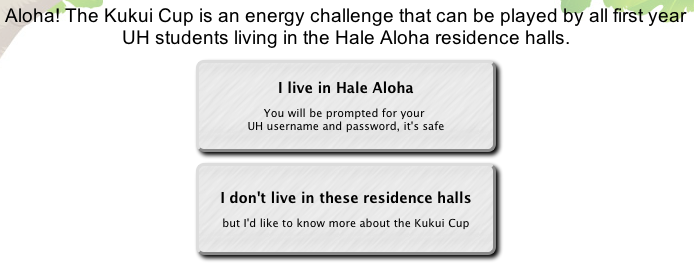
\includegraphics[scale=0.6]{landing-page}
		\caption{A portion of the competition website landing page}
\label{fig:landing-page}
\end{figure}

To provide each participant with personalized information, the competition website required participants to log on with their University of \Hawaii username and password. Using their existing credentials ensured that participants did not have to remember another username and password, which could certainly have been a barrier to participation. The integration was made possible using UH's Central Authentication System. Using a roster provided by UH Student Housing, we were able to prepare accounts for all residents, including which lounge they were living in.

After logging in, new participants were sent through a first-login process. There were seven steps in the process:

\begin{enumerate}
	\item Introduction and chance to verify tower and lounge residence
	\item Terms and conditions, including informed consent
	\item Referral bonus email address entry (see \autoref{referral-bonus})
	\item Profile setup, choosing display name, profile picture
	\item Introductory video, a 2:09 long embedded YouTube video
	\item Question based on introductory video
	\item End of first-login process
\end{enumerate}


\subsubsection{General Page Structure}

After the first-login process is complete, and on all subsequent log-ons, participants were taken to the home page as shown in \autoref{fig:home-page}. The header of the page is shared across all pages on the website. On the left side of the header is the Info Bar, which shows how many points the participant has earned, their standing in the competition, and energy use by their lounge. The Info Bar rotates through the different displays every few seconds. On the right side of the header is the Navigation Bar that contains icons representing the six pages in the website: clicking on the icon takes the user to that page.

\begin{figure}[htbp]
	\centering
		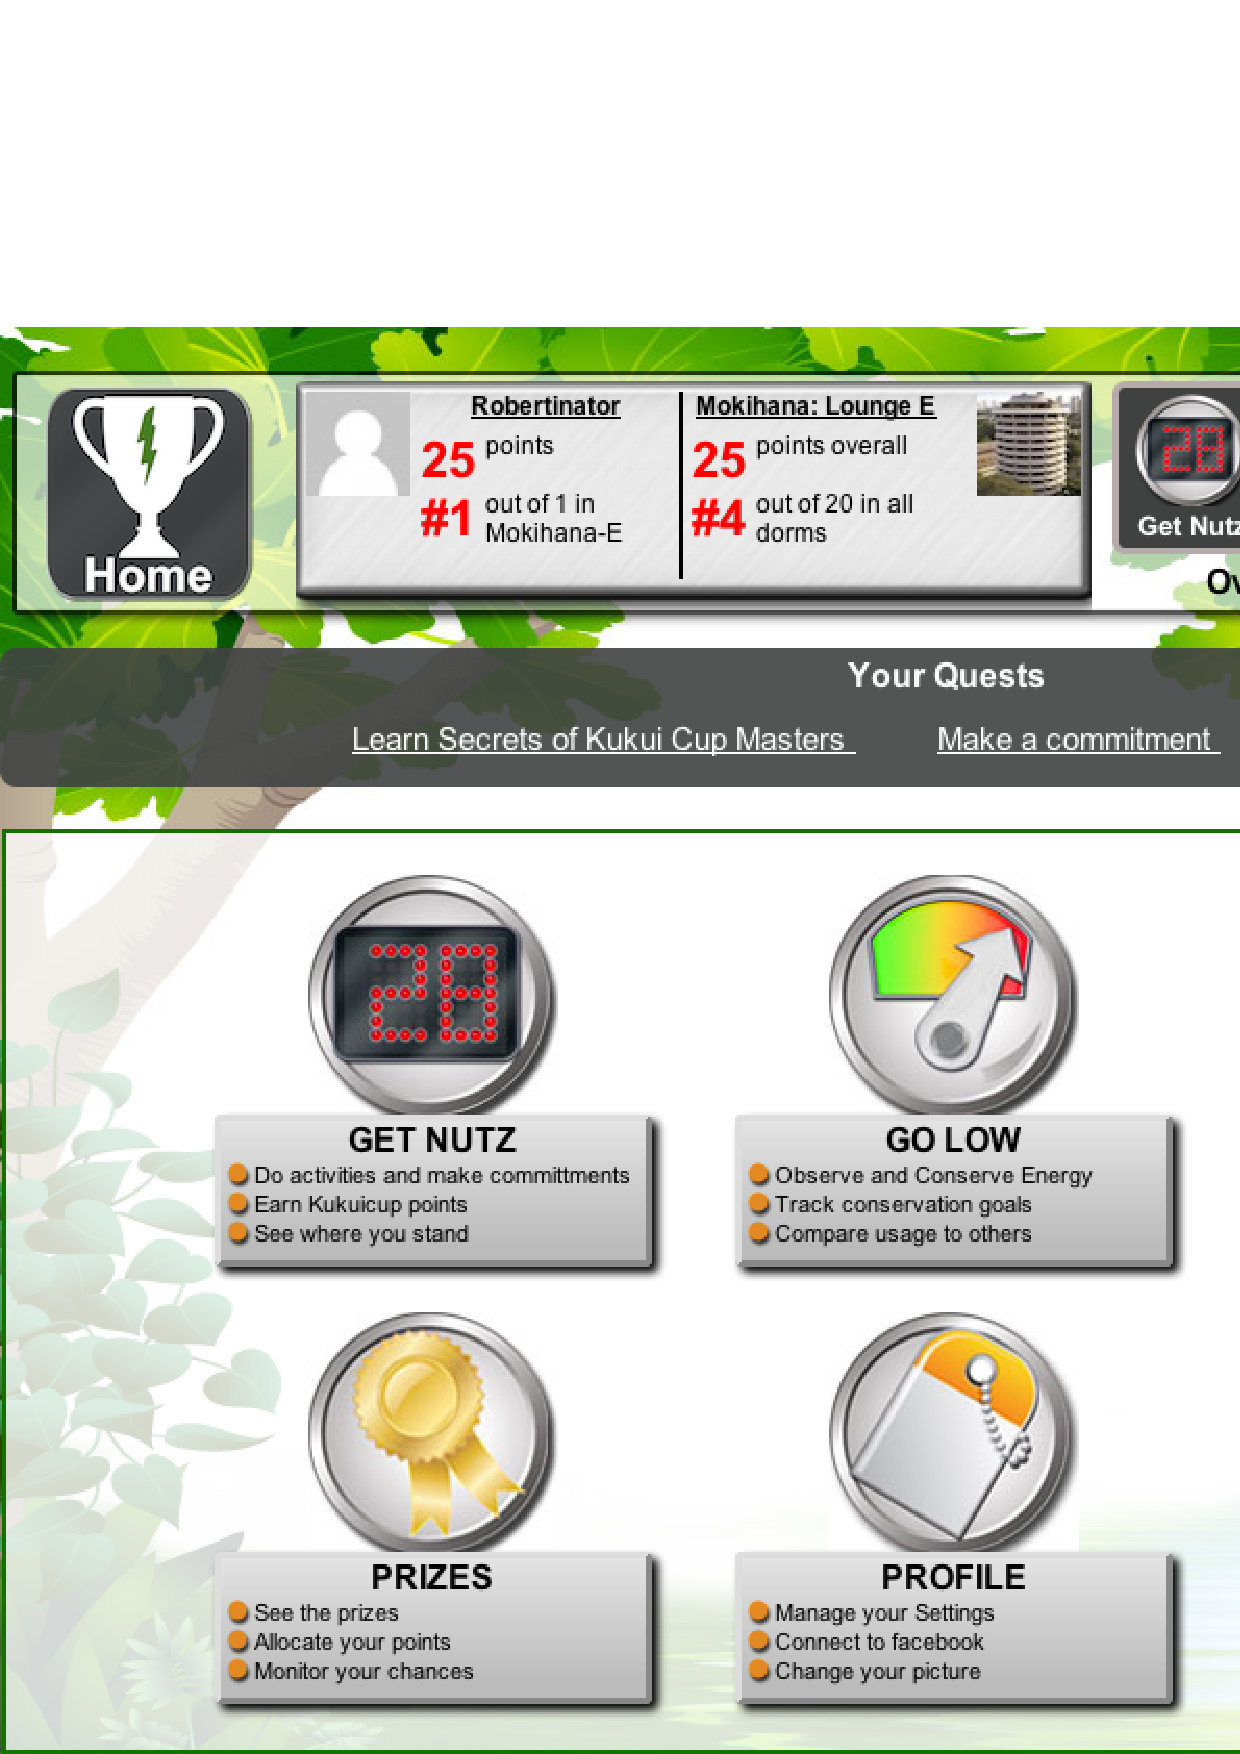
\includegraphics[width=\textwidth]{home-page}
		\caption{The competition website home page}
\label{fig:home-page}
\end{figure}

Below the header is the Quest Bar, which shows the quests available to the participant. We created quests to guide participants through the website and the actions they could take. Each quest has a name, a description, a level, unlock conditions, and completion conditions. The up to three unlocked quests were shown  to participant in the quest bar, ordered by the level of the quest from lowest to highest. If the participant clicked on a quest title, the quest bar expands to show the quest description. After seeing the quest description, participants can choose to accept the quest or close the quest description. Once accepted, the quest is active until the participant meets the completion conditions. Some example quests from the 2011 Kukui Cup were:

\begin{itemize}
	\item ``Learn Secrets of Kukui Cup Masters'', which required participants to watch a video explaining some tips on how best to play the Kukui Cup.
	\item ``Sign up for an event'', which guided participants through the process of signing up to attend their first event.
	\item ``Get the Fully Committed Badge'', which encourages participants to sign up for five commitments, thereby earning the badge.
\end{itemize}

The six pages of the site are:
\begin{itemize}
	\item Get Nutz: take actions for points, view scoreboards
	\item Go Low: real-time energy data, Daily Energy Goal game, energy scoreboard
	\item News: shared lounge ``wall'' (like Facebook) with recent actions taken and discussion
	\item Prizes: list of prizes and Raffle Game
	\item Profile: make changes to display name, view list of past actions taken
	\item Help: rules of competition, frequently asked questions
	\item Canopy: a special area of the site where advanced users can view additional energy visualizations
\end{itemize}

Now I examine each of the pages in turn.


\subsubsection{Get Nutz Page}
\label{sec:get-nutz-page}

The Get Nutz page is the primary place where participants could engage in the point competition. The title of the page refers to the kukui nut that the Kukui Cup is named after. \autoref{fig:get-nutz} shows the a view of the Get Nutz page from the Overall Round of the competition.

\begin{figure}[htbp]
	\centering
		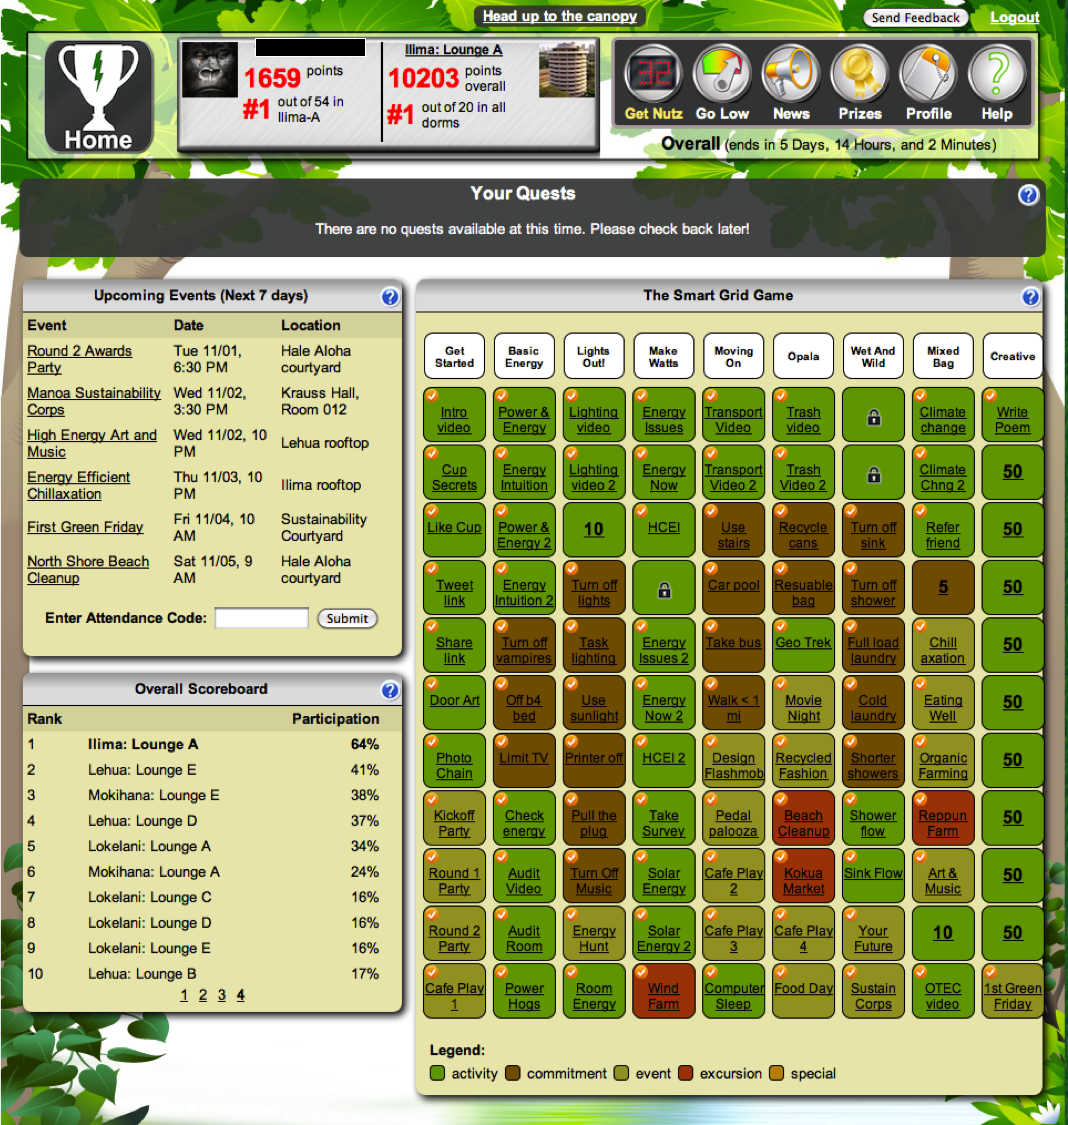
\includegraphics[width=\textwidth]{get-nutz}
		\caption{The Get Nutz point competition page}
\label{fig:get-nutz}
\end{figure}

The main focus of Get Nutz is the Smart Grid Game, which takes up most of the right side of the page. The Smart Grid Game organizes the actions described in \autoref{sec:point-competition} that participants can take to earn points. Each column organizes actions around a particular topic, such as ``Make Watts'' for actions related to energy generation. Each type of action had a different color. Actions that are unlocked display only the point value associated with the action, while locked actions are displayed with a lock icon. Once an action has been completed, the cell displays the name of the action and a small checkmark in the upper-left corner.

On the left side of Get Nutz are the Upcoming Events widget and the Scoreboard widget. Upcoming Events showed events that will take place over the next seven days. Each entry is a link to the event page, which displays details of the event and allows participants to sign up for the event. The Upcoming Events widget also allowed participants to type in event attendance codes directly, without navigating to the event details page.

The Scoreboard widget rotates through four separate scoreboards showing the top ten entries in different categories for the current round: lounge scores, individual scores across all lounges, individual scores within participant's lounge, and participation rates of lounges (see \autoref{sec:active-participation-bonus}).


\subsubsection{Go Low Page}

The Go Low page is the focal point for the energy competition. The page is titled Go Low to remind participants that in the energy competition, the lowest energy use wins (unlike the point competition). \autoref{fig:go-low} shows a view of the Go Low page from the Overall Round of the competition.

\begin{figure}[htbp]
	\centering
		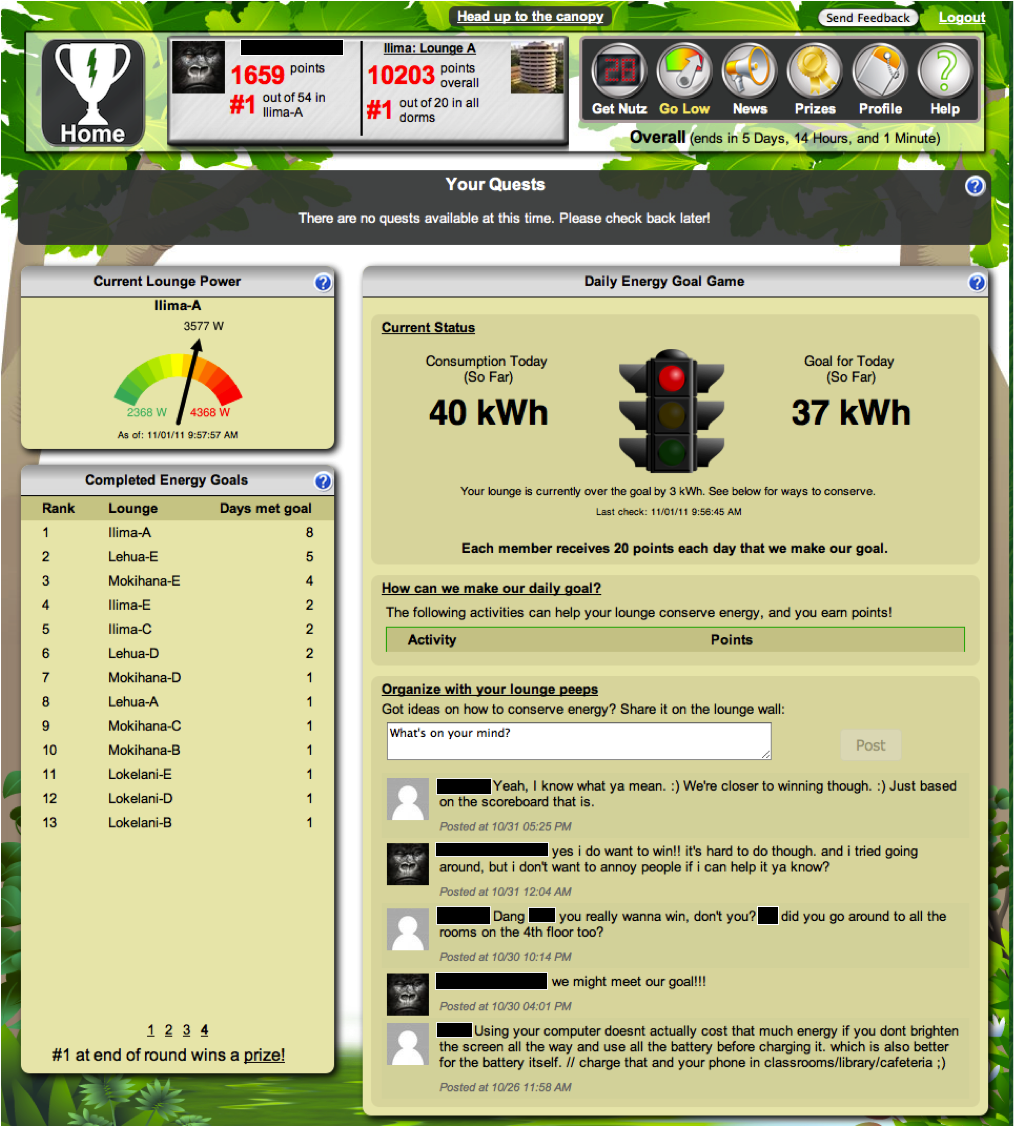
\includegraphics[width=\textwidth]{GoLow-round3}
		\caption{The Go Low energy competition page}
\label{fig:go-low}
\end{figure}

The right side of the page shows the Daily Energy Goal game, described in \autoref{sec:energy-goal-game}. The visualization of the Daily Energy Goal game was implemented in JavaScript, so updates happen dynamically in the browser. To help participants meet their goal, below the Daily Energy Goal game is a section listing actions in the Smart Grid Game related to energy conservation (the list is empty in \autoref{fig:go-low} because the participant has completed all the relevant actions). The bottom portion of the right hand section contains the shared lounge discussion area, called the lounge \emph{wall} after the similar feature in Facebook. Participants can type short messages on the lounge wall that are displayed to all members of the lounge in reverse-chronological order. The wall is intended to assist participants in organizing to reduce their energy usage.

The left side of the page contains the Current Power widget and the Energy Scoreboard widget. The Current Power widget shows the power consumption of the participant's lounge, updated once every 15 seconds. The gauge is calibrated so that the needle pointing directly up corresponds to the average baseline power usage for the current hour of the day. When the needle moves to the right side of the gauge, it represents higher than average power usage for the current time of day, while the left side represents lower than average power usage. The gauge was implemented in JavaScript using the Google Visualization API.\@

The Energy Scoreboard widget ranks all twenty lounges in order of increasing energy use for the current round, and all previous rounds. It also shows a ranking of lounges by the number of energy goals completed by the lounge.


\subsubsection{News Page}
\label{sec:news-page}

The News page of the competition website showed participants what was happening in the competition and in their lounge. \autoref{fig:news-page} shows an example of the News page.

\begin{figure}[htbp]
	\centering
		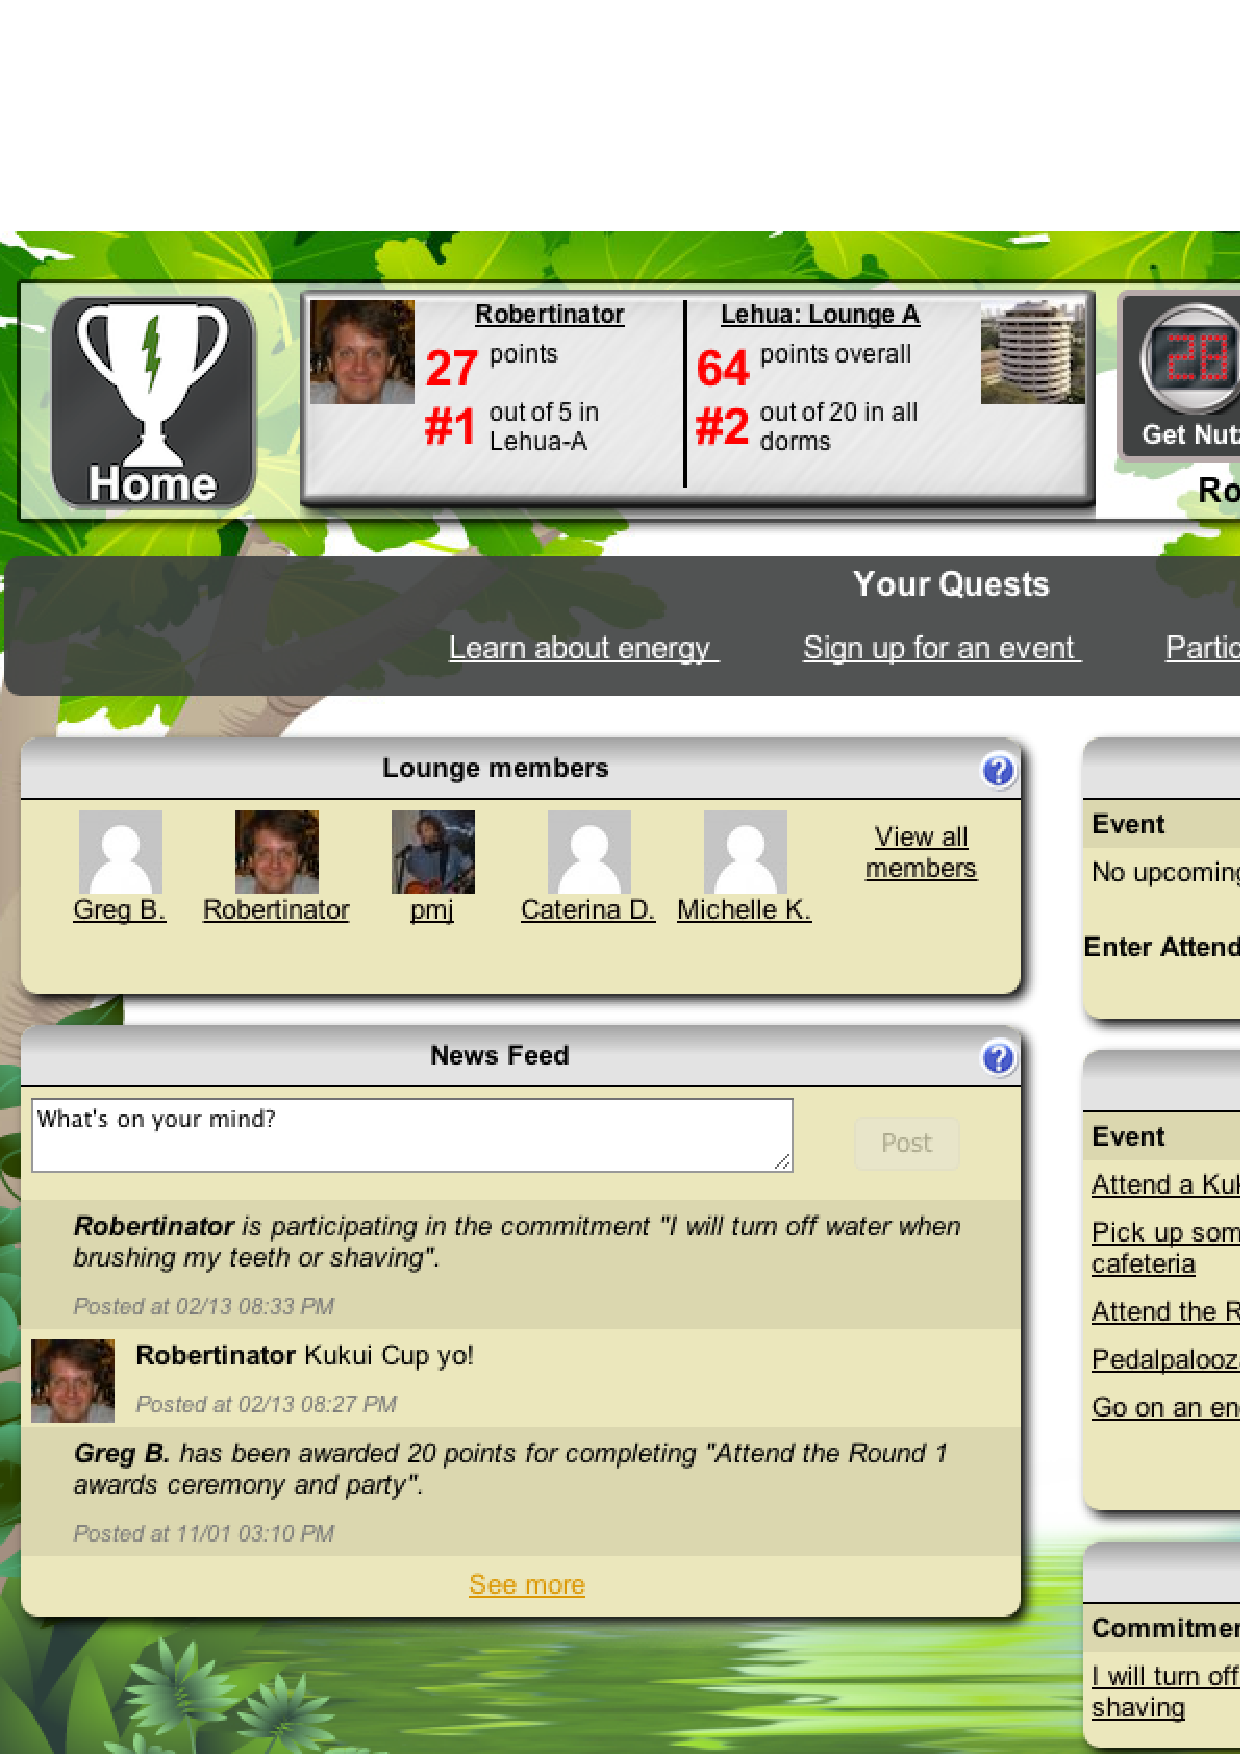
\includegraphics[width=\textwidth]{news-page}
		\caption{The News page of the competition website}
\label{fig:news-page}
\end{figure}

The left column shows two widgets: Lounge members and News Feed. The Lounge members widget shows a subset of the participants in the lounge along with their selected profile picture, with a link to a page showing all the members. The News Feed provides a simple discussion board for lounge members similar to the `wall' concept on Facebook. Participants could type in messages that would be displayed to all other members of the lounge, in reverse chronological order. The system created automated posts when participants performed an action like making a commitment or earning points.

The right column shows three widgets: Upcoming Events, Most Popular, and My Public Commitments. The Upcoming Events widget shows any events taking place today or in the next 7 days. After an event, participants can enter their attendance code directly into the text field to receive points without having to navigate to the specific event page.

The Most Popular widget cycles through a list of events, activities, and commitments ranked in order of how many participants have performed those actions. This widget is intended highlight the popular actions and encourage participants to take part in them. The My Public Commitments widget simply lists the commitments that the participant, which is intended as a reminder to live up to the commitments.


\subsubsection{Prizes Page}

The Prizes page showed participants more information about the incentives available in the competition. \autoref{fig:prizes-page} shows an portion of the Prizes page from the Overall Round of the competition.

\begin{figure}[htbp]
	\centering
		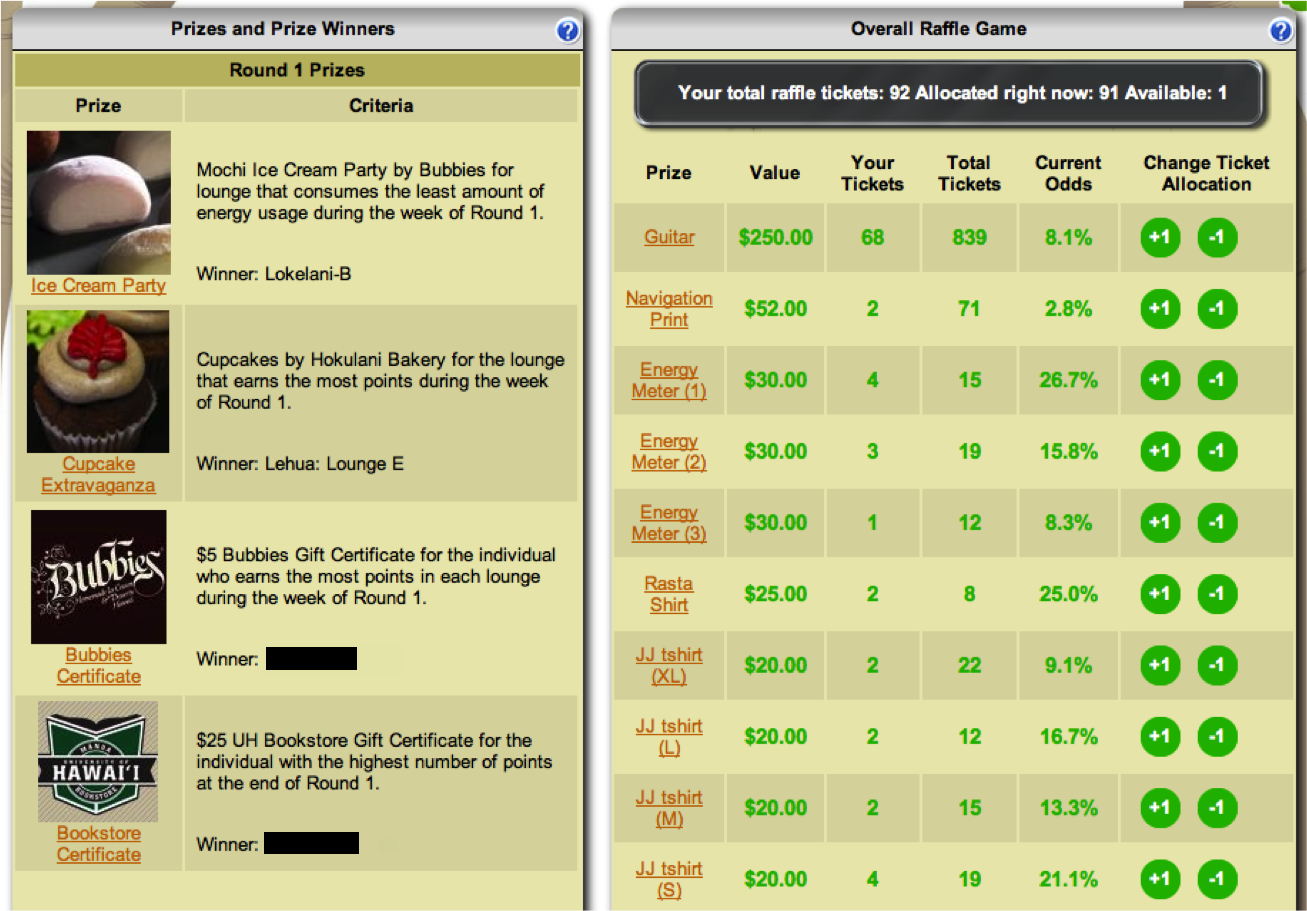
\includegraphics[width=\textwidth]{prizes-page}
		\caption{An excerpt from the Prizes page of the competition website}
\label{fig:prizes-page}
\end{figure}

The left side of the Prizes page shows the prizes awarded to the top participants in each category, as described in \autoref{sec:prizes}. For each prize, the widget showed the lounge or individual in first place for that competition (the currently projected winner). The right side of the prizes page showed the Raffle Game described in \autoref{sec:raffle-game}.


\subsubsection{Profile Page}

The Profile page allowed participants to edit their personal information and view data about their progress in the game. \autoref{fig:profile-page} shows what the Profile page looks like.

\begin{figure}[htbp]
	\centering
		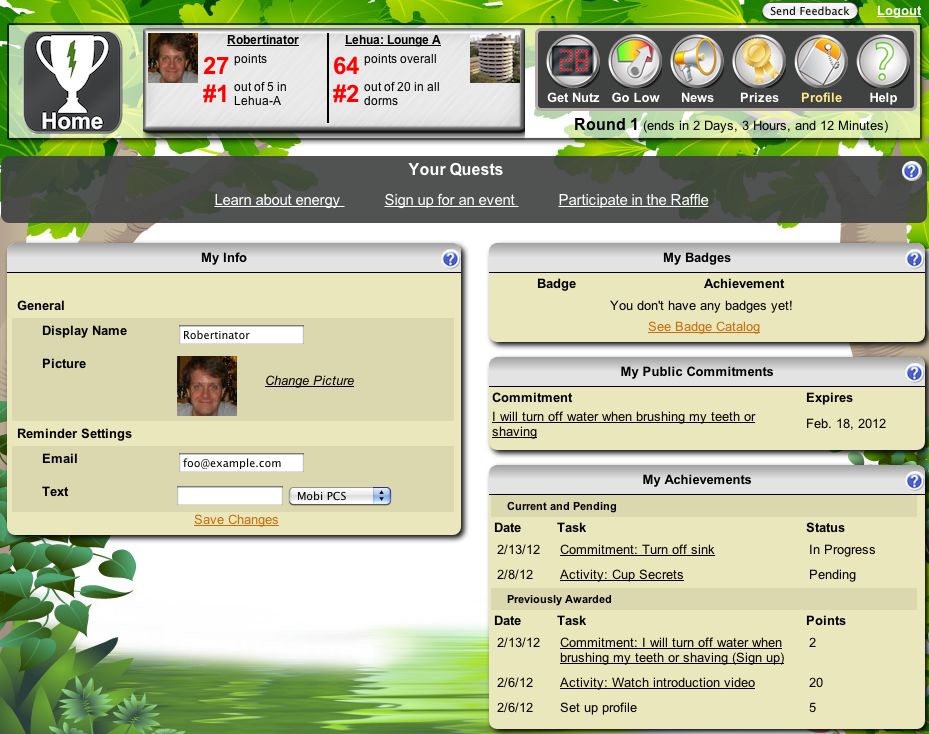
\includegraphics[width=\textwidth]{profile-page}
		\caption{The Profile page of the competition website}
\label{fig:profile-page}
\end{figure}

The left side of the page contains the My Info widget. In My Info, participants could change their display name (used to identify the participant on the website, such as on scoreboards or the lounge News Feed), profile picture, and contact information used when event reminders were requested.

The right side of the page shows competition information for the participant: My Badges, My Public Commitments, and My Achievements. Participants could earn badges for reaching certain goals, such as making five commitments, and the badges earned were displayed in the My Badges widget. My Public Commitments shows the participants commitments (also shown on the News page). My Achievements showed a complete record of all actions taken by the participant in the competition and all points earned.


\subsubsection{Help Page}

The Help page is shown in \autoref{fig:help-page}. On the left side of the page showed the introductory video and links to the rules of the competition. On the right side, one widget showed links to frequently asked questions, and the Ask an Admin widget. Ask an Admin allowed participants to send questions to the competition administrators, which was delivered by email. The Ask an Admin functionality was also available on every page of the website using the Send Feedback button at the top right corner of the page.

\begin{figure}[htbp]
	\centering
		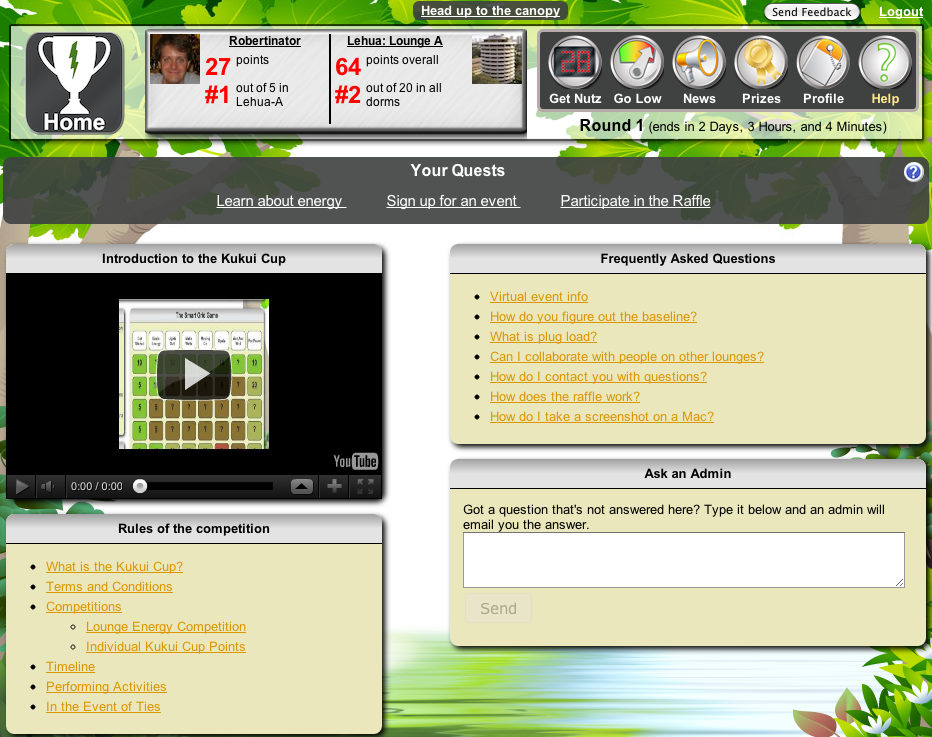
\includegraphics[width=\textwidth]{help-page}
		\caption{The Help page of the competition website}
\label{fig:help-page}
\end{figure}


\subsubsection{The Canopy}

The Canopy was an area of the website designed to provide an additional level of experience for the top participants in the competition. The background of the competition website featured a forest theme, so the Canopy was named to convey that it existed above the rest of the website. Many games feature different levels of difficulty\fxnote{reference for levels of difficulty in games?}, something that was not addressed in the Smart Grid Game. The Canopy was conceived as a way to keep the top participants engaged even if they had earned most of the points available in the Smart Grid Game.

The Canopy was intended to be introduced to top players at the beginning of Round 2 of the competition. The top 50 participants would be sent an email inviting them to a new part of the website. In keeping with the Canopy motif, Canopy members would access the Canopy page by finding a hidden link at top of each web page. The link was hidden until the Canopy member's mouse moved over the link, at which point it was displayed permanently. The ``Head up to the Canopy'' link can be seen at the top of \autoref{fig:help-page}.

\begin{figure}[htbp]
	\centering
		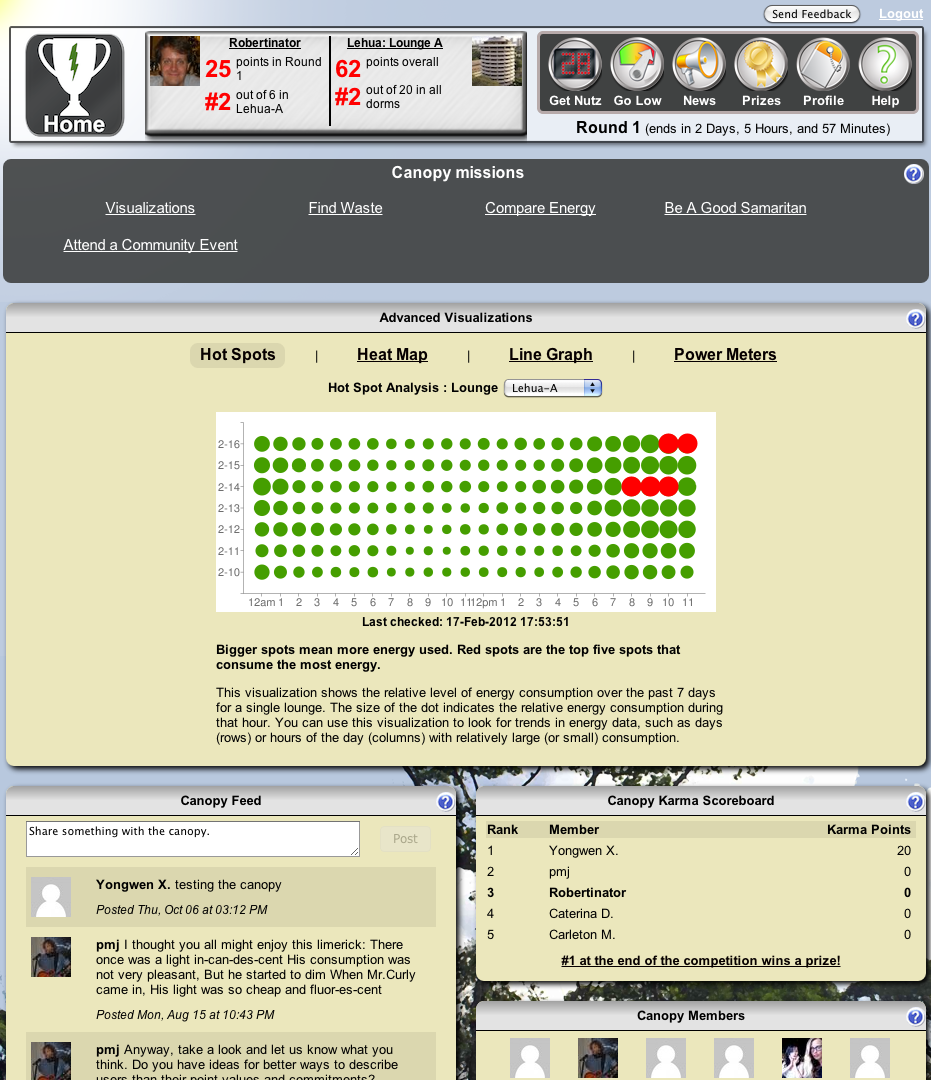
\includegraphics[width=\textwidth]{canopy-page}
		\caption{The Canopy page of the competition website}
\label{fig:canopy-page}
\end{figure}

\autoref{fig:canopy-page} shows the Canopy page itself. The Canopy provided a series of missions, which were displayed just under the header in a similar fashion to the quests in the forest portion of the website. Some Canopy missions were to be accomplished individually, while other missions required 2 or 3 participants to work together. Participants could indicate that they were ``up'' for a group mission to find other interested participants.

The Canopy missions contained links to Canopy activities. Canopy activities were like forest activities (see \autoref{sec:activities}), but instead of earning points upon completion, Canopy activities earn \emph{Canopy Karma}, which was a separate point system for the Canopy. Canopy Karma was used instead of the standard points to ensure that the Canopy itself did not unbalance the point competition by providing a way for the top players to earn more points that were not available to the rest of the participants.

The energy data and visualizations shown on the Go Low page were deliberately simple to avoid confusing participants, based on the results of usability testing. In addition, the detailed energy data shown on Go Low comes only from the participant's lounge. Since the Canopy was intended for the top participants of the competition, who were believed to be more receptive to detailed energy data and data for other lounges, energy visualizations feature prominently in the Canopy. Several of the Canopy activities involved looking at the advanced visualizations and answering questions based on their understanding of the data.

Since the members of Canopy cut across different lounges, a special Canopy Feed discussion board was provided to allow collaboration. The Canopy Feed worked in the same way the lounge News Feed described in \autoref{sec:news-page}. The Canopy also featured a Canopy Karma scoreboard showing the top participants in the Canopy, and a \$25 UH Bookstore gift card was offered as a prize to the participant with the most Canopy Karma at the end of the competition.


\subsection{Energy Data Integration}
\label{sec:energy-data-integration}

The energy data for the competition was stored in a WattDepot server. Before and during the competition, the energy meters were queried at approximately 15 second intervals. After the competition was over, there was no need for real-time data, so I increased the query interval to 5 minutes.

The competition website has several areas that require access to energy and power data: the Daily Energy Goal Game, the Current Power gauge, and the Energy Scoreboards. Since each of these components run in the browser and dynamically update, the load on the WattDepot server could be proportional to the number of participants in the competition. To reduce the potential load on on the WattDepot server, Professor Philip Johnson wrote a system called WattDepot-GData~\cite{wattdepot-gdata}, which periodically queries a WattDepot server and stores the results in a Google Docs spreadsheet. The spreadsheets created by WattDepot-GData are structured to meet the needs of the Makahiki visualizations, such as the total energy use since the beginning of the current round of the competition. Using Google Docs to store the data in the cloud also insulates the WattDepot server from heavy client loads.

\chapter{Experimental evaluation} \label{experiments}
Three case studies: a pilot study, a classroom case study, and a public data case study will be conducted in order to empirically evaluate capabilities and performance of the Hackystat Trajectory framework. A pilot study is ongoing along with development of the framework and some of the results discussed in this chapter.

The primary goal of these studies is to assess the ability of the framework to reproduce well known recurrent behavioral patterns (for example TDD), as well as the ability to discover novel ones. As the secondary goal, I see the classification and extension of the current Hackystat sensors family in order to improve the system performance. It is quite possible that some of the currently collected sensor data will be excluded from the Trajectory Analysis datasets, while some new ones will be designed and developed in order to capture important features from software process. 

\section{Pilot study}\label{pilot.evaluation}
In order to demonstrate the ability of the current framework implementation to perform telemetry indexing and temporal recurrent patterns extraction, I have conducted two pilot experiments discussed next. 

\begin{figure}[tbp]
   \centering
   \includegraphics[height=185mm]{cluster_streams.eps}
   \caption{Clustering of telemetry streams for classroom pilot dataset using symbolic approximation and vectors of motif frequencies. While it seems to be meaningful to find correlation between \textit{UnitTest\_Failure} and \textit{CodeIssue} streams unit test, this grouping happened due to the similarity of behavior pattern - short, hight in amplitude bursts; but note, there is no correlation in time.}
   \label{fig:cluster_streams}
\end{figure}

\subsection{Clustering of the Hackystat Telemetry streams}
The main purpose of the first pilot study was to evaluate the ability of PAA and SAX approximations to capture recurrent temporal patterns in telemetry streams. Knowing about usually misleading results of time-series clustering \cite{citeulike:227029}, I did not expect to capture much interesting facts, nevertheless the results were encouraging.

For pilot study I used real data collected during the Spring'09 software engineering class. This dataset represents Hackystat metrics collected during sixty days of a classroom project development conducted by eight students. The following clustering experiments were conducted using the distance between vectors of motif frequencies:
\begin{itemize}
	\item Clustering of software process related telemetry streams collected from individual developers. I was able to group developers with the similar behavioral patterns within clusters, which indicates the correctness of the classification approach.
	\item Clustering of software product-related telemetry streams by using shared motif frequencies. As a result of this experiment, I was able to group telemetry streams, but while stream groups look intuitively meaningful, close examination of the streams indicates that this grouping happened just because of the method applied. The results indicate that instead of using just motif frequencies, some temporal ordering should be taken into account.
\end{itemize}

\subsection{Sequential patterns search}
The second pilot study, aiming at discovery of sequential patterns, was also conducted using real data from my own concurrent development of two software projects. While working on the Hackystat Trajectory framework, I made decision to split the code into two parts: an algorithm implementation library that I named JMotif, and the user-interface part called TrajectoryBrowser. While this decision simplified development, it introduced a heavy dependency of TrajectoryBrowser on the JMotif API, which provides variations of DTW, PAA and SAX algorithms along with defining data structures for indexing and clustering. As a result of iterative and incremental pattern in my development, I changed the JMotif public API three times, which consequently involved extensive refactoring in the ProjectBrowser code. This dependency can be clearly seen from observing DevTime streams at Figure \ref{fig:sequential_growth} panel $a$. 

\begin{figure}[tbp]
   \centering
   \includegraphics[height=80mm]{sequential_growth.eps}
   \caption{The illustration of finding of sequential $growth \; pattern$ in two DevTime telemetry streams. Panel $a$: The Hackystat ProjectBrowser showing telemetry streams. Panel $b$: the TrajectoryBrowser showing same telemetry streams along with identified pattern. Panel $c$: the symbolic representation of streams with highlighted pattern.}
   \label{fig:sequential_growth}
\end{figure}

In order to capture this dependency pattern in two Telemetry streams, representing daily amount of development time spent on the TrajectoryBrowser and JMotif projects, I defined a synthetic \textit{growth pattern} as the large positive delta value between previous and current day effort. By transforming Telemetry streams with this simple rule in the symbolic form, I obtained a two dimensional symbolic time series, where letter $G$ represents a growth pattern, see Figure \ref{fig:sequential_growth} panel $c$. I have defined a formal rule for \textit{sequential growth} pattern as the pattern like $G_{JMotif}\; \rightarrow \; G_{TrajectoryBrowser}$ where distance between these $G$s is less than three days. By application of this rule I identified a pattern which exactly corresponds to my experience.

\chapter{Conclusion}
\label{cha:conclusion}

This research investigates the information technology infrastructure that can support effective and efficient development of serious games for sustainability. The research includes the development of an innovative serious game framework for sustainability that combining education and behavior change, and an assessment method accessing the effectiveness and efficiency of the IT infrastructure for serious games for sustainability with regarding the most important stakeholder's perspective.

\section{Contributions}

The contributions of this research are:

\begin{itemize}
	\item Makahiki: open source information technology for development of serious games for sustainability.
	\item SGSEAM: an assessment method for assessing serious game framework.
	\item Evidence regarding the effectiveness and efficiency of Makahiki as a framework for development of serious games for sustainability.
	\item Evidence regarding the effectiveness and efficiency of a second system (BuildingOS) as a framework for development of serious games for sustainability.
	\item Insights into the strengths and weaknesses of the assessment method.
\end{itemize}

\section{Future Directions}

There are a variety of directions that can be pursued once this research is complete, such as:

\begin{itemize}
	\item Evaluate the other stakeholders’ experiences

    \item Build a community to expand content and game library for Makahiki

    \item Scale and expand Makahiki to support other geographical and cultural different locations.

\end{itemize}



%%% Switch to appendix mode
\appendix
%%% Bring in any appendices from external files
\chapter{Physical Concepts: Power and Energy}
\label{app:power-energy}

When discussing energy, and in particular electricity, it is important to understand what power and energy are, and how they interrelate.

\section{Energy}

Energy is defined as the amount of work that can be done by a force. Most of us have an intuitive notion of energy: is makes things move, it heats things up, etc. There are many units used to measure energy: joules (a very small amount of energy), BTUs, calories. When talking about electricity, the most common unit is the watt hour, abbreviated as "Wh", which is equal to 3600 joules. A watt hour is the amount of energy required to to provide 1 watt of power for one hour. Note that from a certain perspective it is somewhat peculiar to measure energy in units that include power (watt), since power is defined in terms of energy in the first place. This underlines how central the concept of power is in most of our dealings with electricity.

\section{Power}

Power is defined as the rate of change for energy. As with any rate, it is expressed as a quantity of energy over a unit of time. The most common unit for power is the watt, abbreviated as "W". One watt is defined as one joule (a measure of energy) per second. You might be familiar with a 60 watt incandescent light bulb, which expresses how much power it uses when turned on.

\section{Analogy To Cars}

Power and energy are closely related, but frequently confused concepts. As an analogy, think about a car. We can talk about the speed of a car (in miles per hour, or kilometers per hour) and we can also talk about a distance driven in a car (miles or kilometers). The speedometer in the car measures the speed (distance over time), while the odometer measures the distance traveled. Speed is a rate, like power, while distance is like energy.

When we talk about speeds, we usually talk about instantaneous measurements of speed. A speed limit is the maximum instantaneous speed at which you are allowed to drive, i.e. the car's speedometer should never register a speed greater than the limit. However, when we talk about distance driven, it only makes sense to talk about a distance driven between two locations, or the distance driven over a particular time interval. There is no such thing as an instantaneous distance driven, because in at a precise instant in time, the car is not moving.

\section{Power vs. Energy}

Since power is the rate of change of energy, if you know how power changes over time, you can determine how much energy was consumed or produced (the area under the power curve). Similarly, if you know how much energy was used over an interval of time, you can compute the average power over that period of time (but not the instantaneous power).

In our interactions with appliances, we usually talk about their power consumption and not their energy consumption. For example, we have 60 watt light bulbs, but we wouldn't generally talk about a 60 watt hour lightbulb (unless it consumed 60 watts for an hour and then burned out!). This is because power consumption is an intrinsic characteristic of things that use electricity, while the amount of energy used by an electrical device is determined by how long you keep it plugged in or turned on. On the other hand, energy is very important to the utility that provides your electricity, since you are billed by how much energy you have used (typically in kilowatt hours).

The two key points to remember are: power is a rate, and we always talk about energy over an interval of time.

%%%%%%%%%%%%%%%%%%%%%%%%%%%%%% -*- Mode: Latex -*- %%%%%%%%%%%%%%%%%%%%%%%%%%%%
%% uhtest-appendix.tex -- 
%% Author          : Robert Brewer
%% Created On      : Fri Oct  2 16:31:12 1998
%% Last Modified By: Robert Brewer
%% Last Modified On: Mon Oct  5 14:41:05 1998
%% RCS: $Id: uhtest-appendix.tex,v 1.1 1998/10/06 02:07:03 rbrewer Exp $
%%%%%%%%%%%%%%%%%%%%%%%%%%%%%%%%%%%%%%%%%%%%%%%%%%%%%%%%%%%%%%%%%%%%%%%%%%%%%%%
%%   Copyright (C) 1998 Robert Brewer
%%%%%%%%%%%%%%%%%%%%%%%%%%%%%%%%%%%%%%%%%%%%%%%%%%%%%%%%%%%%%%%%%%%%%%%%%%%%%%%
%% 

\chapter{Participant Kukui Nut Tasks}
\label{app:tasks}

This appendix lists tasks intended to be undertaken by the competition participants. Each task should increase the energy literacy of the participants performing it, help them modify their behavior to reduce electricity usage, or both. The following lists all the possible tasks, and indicate how they would be performed, validated, and what the potential benefit would be to the person performing it. The tasks are grouped into four categories: events, activities, commitments, and goals. For more information, see \autoref{sec:competition-tasks}.


\section{Events}

One common type of task is attendance of an event. In our model, there are two ways to get credit for attending an event: activities (individual attendance), and goals (floor attendance). Since the parameters are often identical between the activity version and the goal version of an event, they are grouped together here.

For both event activities and goals, attendance is verified using non-forgeable, single-use attendance codes such as "orientation-158-B7QRX13". The codes are printed on small slips of paper that are handed out by some responsible person who is not a participant (such as the event speaker or an RA).

In the case of activities, to get credit for attending, the individual participant logs into the web site and enters in the attendance code. The website automatically awards KN points if the attendance code is valid, and it has not already been entered.

For goals, the participant that initiated the goal must log into the website after the event and indicate that the goal was met (perhaps prodding any floormates to enter their attendance codes if they haven't alread done so). The website will then award the appropriate KNs to all members of the floor (including those who did not attend). Goals must have the participation of at least half of the floor participants to be successful. If a floor achieves 100\% participation, they receive double the KN.

Relatively passive events like movies or lectures should be worth around 5 KN, while more interactive events like workshops should be worth more (perhaps 10-15 KN).

\subsection{Attend Kukui Cup orientation}

Description: Participant attends a large orientation meeting about the Kukui Cup competition.

Potential benefits: Understanding of the competition mechanics, collaboration with other floor participants on competition strategy.

Psychological justifications: ?

Activity reward: 4 KN

Goal reward: 5 KN (unlikely to be obtained, since this happens at very begining of competition)

\subsection{Attend EnergyPong tournament}

Description: Participant attends the EnergyPong tournament for their building.

Potential benefits: Improved energy literacy through hearing energy questions answered, floor bonding.

Psychological justifications: competition

Activity reward: 2 KN

Goal reward: 4 KN

\subsection{Attend a special Kukui Cup SustainableUH meeting}

Description: Participant attends a special presentation by SustainableUH team members on what SustainableUH is doing on campus.

Potential benefits: Getting involved with peers on campus, learning what challenges exist and how students are working to overcome them.

Psychological justifications: ?

Activity reward: 2 KN

Goal reward: 5 KN

\subsection{Watch the movie "Who Killed the Electric Car"}

Description: Participant watches the movie.

Potential benefits: Understanding of the possibility of de-carbonizing transportation, difficulty of changing status quo.

Activity reward: 2 KN

Goal reward: 5 KN

\subsection{Watch the movie "Enron: The Smartest Guys in the Room"}

Description: Participant watches the movie.

Potential benefits: Understanding risks and problems from utility deregulation, ethical issues.

Activity reward: 2 KN

Goal reward: 5 KN

\subsection[Watch the movie ``The End of Suburbia'']{Watch the movie ``The End of Suburbia''}

Description: Participant watches the movie.

Potential benefits: Understanding peak oil, design of communities around automotive transportation and plentiful cheap energy.

Activity reward: 2 KN

Goal reward: 5 KN

\subsection{Watch the movie "A Crude Awakening: Oil Crash"}

Description: Participant watches the movie.

Potential benefits: Understanding peak oil, consequences for society.

Activity reward: 2 KN

Goal reward: 5 KN

\subsection{Watch the movie "The Great Warming"}

Description: Participant watches the movie.

Potential benefits: Understanding climate change, consequences for society.

Activity reward: 2 KN

Goal reward: 5 KN

\subsection{Watch the movie "An Inconvenient Truth"}

Description: Participant watches the movie.

Potential benefits: Understanding climate change, consequences for society.

Activity reward: 2 KN

Goal reward: 5 KN

\subsection{Participate in a 10/10/10 work party}

Description: [http://www.350.org/ 350.org], a climate change advocacy organization is organizing a series of "work parties" to take place on October 10, 2010 (10/10/10). Participant participates in a work party in Honolulu (check website for options). Since this is off campus, might need to support alternate verification (photo and text) instead of attendance codes.

Potential benefits: Understanding climate change, consequences for society.

Activity reward: 5 KN

Goal reward: 7 KN


\section{Activities}

\subsection{Perform room energy audit}

Description: Resident borrows a Kill-A-Watt plug load meter from their RA, then checks all plug-in appliances in their room to see what their energy consumption is when on and off.

Verification: Participant fills out form on website that contains a list of rows for each device with columns: device name, power (watts) when off, power (watts) when on, notes. Admin reviews data, checking mainly for completeness (more than 1 device?) and sanity (XBox 360s don't use 1000 W).

Reward: 10 KN

Potential benefits: Increased intuitive understanding of the watt, familiarity with vampire power, understanding of how device usage would impact energy consumption, reduced electricity usage due to turning off devices when not in use.

Psychological justifications: feedback, activity-based learning (?)

\subsection{Replace incandescent bulb with compact fluorescent (CFL)}

Description: Participant finds an incandescent bulb (perhaps from a desk lamp) and replaces it with a CFL, throwing away the incandescent bulb.

Verification: Participant takes a picture showing both the incandescent bulb and the CFL replacement and uploads it via a verification form on the website, along with a text field indicating where the replaced bulb is located. Admin briefly reviews the picture to ensure that in fact both bulbs are present.

Reward: 3 KN

Potential benefits: Reduced energy usage via CFL, awareness of energy impact of incandescent bulbs.

Psychological justifications: activity-based learning (?)

\subsection{Configure computer \& monitor to sleep after inactivity}

Description: Participant configures their computer and any external display to sleep after 20 minutes of inactivity.

Verification: Participant takes a screenshot from their computer showing sleep settings <= 20 minutes and uploads it via a verification form on the website. Admin briefly reviews the picture to ensure that the settings look correct.

Reward: 3 KN

Potential benefits: Reduced computer \& monitor energy usage, knowledge of how to set it up on other computers (friends, work, future purchases, etc).

Psychological justifications: none

\subsection{Play in EnergyPong tournament}

Description: Participant is on their floor's team in the EnergyPong tournament for their building.

Verification: Some responsible person who is not a participant (such as the speaker or an RA) records attendance and performance, which is reported to the website admins either on paper or via email.

Reward: 4 KN + 1 KN per bracket completed + 5 KN for the winning team

Potential benefits: Improved energy literacy through answering energy questions answered, floor bonding.

Psychological justifications: competition, incentives (if prizes are awarded to winning team)

\subsection{Connect to Kukui Cup on Facebook}

Description: Participant becomes a fan of the Kukui Cup Competition group on Facebook.

Verification: Participant takes a screenshot from their computer showing Facebook fan status. Admin briefly reviews the picture to ensure that the participant is a fan.

Reward: 3 KN

Potential benefits: Another avenue for communicating with students, promotion of the contest and energy literacy.

Psychological justifications: community involvement?

\subsection{Tweet about Kukui Cup}

Description: Participant sends a tweet promoting the Kukui Cup Competition with a link to the website.

Verification: Participant takes a screenshot from their computer showing the tweet in their newsfeed. Admin briefly reviews the picture to ensure that the participant tweeted.

Reward: 2 KN

Potential benefits: Promotion of the contest and energy literacy.

Psychological justifications: social networking?

\subsection{Facebook Status update about Kukui Cup}

Description: Participant updates their Facebook status promoting the Kukui Cup Competition with a link to the website.

Verification: Participant takes a screenshot from their computer showing the status in their newsfeed. Admin briefly reviews the picture to ensure that the participant updated their status.

Reward: 2 KN

Potential benefits: Promotion of the contest and energy literacy.

Psychological justifications: social networking?

\subsection{Label all plug loads in room}

Description: Followup to room energy audit. Based on the audit results, make a label for each device with the number of watts consumed when on and off, located close to the power switch for those devices that have them.

Verification: Participant takes a picture of the devices with their labels. Admin briefly reviews the picture to ensure that labels are present.

Reward: 3 KN

Potential benefits: understanding of how device usage would impact energy consumption, reduced electricity usage due to turning off devices when not in use.

Psychological justifications: prompts

\subsection{Determine carbon footprint using calculator}

Description: Participant uses a web-based carbon footprint calculator to determine their carbon footprint.

Verification: Participant enters in their computed carbon footprint into a text field. Admin briefly reviews the footprint to make sure it is sane (units include CO2 and it isn't huge or tiny).

Reward: 3 KN

Potential benefits: learning about carbon emissions, learning how carbon emissions impact the environment.

Psychological justifications: personalized data


\section{Commitments}

Note that per the requirements, commitments are participant-verified without outside intervention, so that field is not used for this category.

\subsection{Turn off lights when I leave the room}

Description: The participant commits to turning off all lights whenever they are the last person to leave a room.

Reward: 2 KN

Potential benefits: Reduced electricity usage due to less unneeded lighting, highly obvious reminder of need to conserve energy.

Psychological justifications: public commitments

\subsection{Use task lighting instead of overhead lights}

Description: The participant commits to using task lighting (i.e. a desk lamp) instead of overhead room lights. Might only be appropriate if housing rooms have overhead lights.

Reward: 2 KN

Potential benefits: Reduced electricity usage due to less excess lighting.

Psychological justifications: public commitments

\subsection{Always disconnect vampire loads using a power strip}

Description: The participant commits to turning off any vampire loads (cell phone charger, iPod charger, game consoles, TVs) using a power strip when they are not using them.

Reward: 2 KN

Potential benefits: Reduced electricity usage due to vampire loads, awareness of vampire loads.

Psychological justifications: public commitments

\subsection{Turn off water when brushing teeth, shaving, etc}

Description: The participant commits to turning off any vampire loads (cell phone charger, iPod charger, game consoles, TVs) using a power strip when they are not using them.

Reward: 2 KN

Potential benefits: Reduced electricity usage due to vampire loads, awareness of vampire loads.

Psychological justifications: public commitments

\subsection{Turn off water when sudsing and scrubbing in shower}

Description: The participant commits to turning off water when showering except when actively rinsing off.

Reward: 2 KN

Potential benefits: Reduced electricity usage due to less water heating and pumping.

Psychological justifications: public commitments

\subsection{Use natural light instead of electric lighting whenever possible}

Description: The participant commits to using natural light from windows or outdoors instead of turning on electric lighting. This can mean opening shades instead of turning on the lights, and/or planning their day so that tasks that require light (like reading books, doing written homework) are done during the day.

Reward: 2 KN

Potential benefits: Reduced electricity usage due to less use of electric lights.

Psychological justifications: public commitments

\subsection{Turn off printer when not printing}

Description: The participant commits to turning off their printer when they are not actively printing out documents.

Reward: 2 KN

Potential benefits: Reduced electricity usage due to less standby electricity for printer.

Psychological justifications: public commitments

\subsection{Use stairs instead of elevator}

Description: The participant commits to using the stairs instead of elevators whenever feasible.

Reward: 2 KN

Potential benefits: Reduced electricity usage due to less elevator traffic. Increased exercise for participant.

Psychological justifications: public commitments

\subsection{Recycle all beverage containers}

Description: The participant commits recycling all (recyclable) beverage containers at an appropriate location.

Reward: 2 KN

Potential benefits: Reduced carbon emissions due to recovery and eventual reuse of recyclable material, reduction in waste stream.

Psychological justifications: public commitments

\subsection{Don't drive off-campus using a single-occupant car}

Description: The participant commits to not traveling off-campus in single-occupant car, using bus, bike, walking, or vehicle with 3+ occupants instead.

Reward: 2 KN

Potential benefits: Reduced carbon emissions due to less single occupant car travel, reduction in traffic and parking.

Psychological justifications: public commitments

\subsection{Turn off/shut down all appliances before going to sleep}

Description: The participant commits to turning off or shutting down appliances like computers, TVs, DVD players, and game consoles before going to sleep each night.

Reward: 2 KN

Potential benefits: Less electricity wasted on appliances that aren't being used.

Psychological justifications: public commitments

\subsection{Limit TV watching to 1 hour a day or less}

Description: The participant commits to watching not more than 1 hour of TV per day.

Reward: 2 KN

Potential benefits: Less electricity used by television.

Psychological justifications: public commitments

\subsection{Do only full loads of laundry}

Description: The participant commits to always doing full loads of laundry.

Reward: 2 KN

Potential benefits: Less electricity \& hot water used per piece of laundry washed.

Psychological justifications: public commitments

\subsection{Wear Kukui Cup button every day}

Description: The participant commits to wearing their Kukui Cup button every day during the commitment period.

Reward: 2 KN

Potential benefits: promotion of the contest.

Psychological justifications: public commitments

\subsection{Walk to destinations less than one mile away}

Description: The participant commits to walking to any destination less than one mile away from their residence hall.

Reward: 2 KN

Potential benefits: Reduced gasoline usage due to car usage. Increased exercise for participant.

Psychological justifications: public commitments

\subsection{Wash laundry in cold water}

Description: The participant commits to washing laundry in cold water instead of warm or hot water.

Reward: 2 KN

Potential benefits: Reduced electricity usage by reduction in water heating and pumping.

Psychological justifications: public commitments

\subsection{Reduce the shower time by 1 minute}

Description: The participant commits to measuring the length of their shower with a watch, and reducing the time by 1 minute.

Reward: 2 KN

Potential benefits: Reduced electricity usage by reduction in water heating and pumping.

Psychological justifications: public commitments

\subsection{Turn off music when leaving room}

Description: The participant commits to turning off their music (from computer, stereo, etc) when they leave the room.

Reward: 2 KN

Potential benefits: Reduced electricity usage.

Psychological justifications: public commitments

\subsection[Do something ``unplugged'' every day]{Do something ``unplugged'' every day}

Description: The participant commits to doing something that doesn't require electricity instead of watching TV, using their computer, or playing a console game.

Reward: 2 KN

Potential benefits: Reduced electricity usage, increased exercise?

Psychological justifications: public commitments

\subsection{Bring reusable bags when shopping}

Description: The participant commits to bringing and using reuseable bags when shopping instead of the paper or plastic ones offered by the store.

Reward: 2 KN

Potential benefits: Reduced waste, reduced carbon footprint.

Psychological justifications: public commitments

\subsection{Don't eat meat}

Description: The participant commits to not eating any meat (beef, pork, chicken, fish, shellfish, etc) for the commitment period.

Reward: 2 KN

Potential benefits: Reduced carbon footprint, potentially improved health.

Psychological justifications: public commitments


\section{Goals}

\subsection{Reduce our floor's energy consumption by {target} }

Description: A floor participant picks a target goal (hopefully in consultation with rest of floor) for reduction for the current period from a list of choices from 5\% to 50\% in 5\% increments.  When the goal is specified, the system uses the Average Floor Power as the value being reduced from.  The system can provide a graphic that is updated in near-real time to show whether (a) the current usage is above or below the target, and (b) whether the cumulative usage so far is above or below the target.  The graphic can also provide a count-down timer showing the time remaining to achieve this goal in days:hours:minutes.

Note that the percentage reduction is always relative to the baseline, not the prior week.  So, a floor might start out with a conservative goal of 5\%, then find that they actually achieved 16\% during the period. So, they could restart the goal for the next period, this time choosing 15\%.

Verification: Participant that picked the goal must use the web interface indicate that the goal has been met or not met, and an admin assigns points accordingly.

Reward: If the floor achieves the target reduction, then each member of the floor is awarded 1 KN per target percentage reduction. For example, if the target reduction was 5\% and the floor achieved 7\%, then each member gets 5 KNs for achieving this goal.

Potential benefits: Reduced electricity usage, group planning for how to achieve target through behavior changes.

Psychological justifications: goal setting with feedback, social norms

\subsection{Finding the minimum floor power}

Description: A floor participant picks a day and time for the floor to try to determine the minimum amount of power the floor can consume. Everyone on the floor must disconnect and unplug all loads, all lights must be turned off, etc. Then, using a laptop or mobile device, the floor's instantaneous power value is recorded from the monitors on the contest website.

Note that this goal requires near 100\% participation to be successful.

Verification: Participant that picked the goal must use the web interface indicate what power value the floor was able to record. The admin can then compare this to the [NormalizingPowerData Minimum Floor Power]. If the participants got within 10\% of the MFP, then the KN are awarded.

Reward: Each member gets 10 KNs for achieving this goal.

Potential benefits: Awareness of building infrastructure power draws, group collaboration to turn everything off, awareness of vampire loads.

Psychological justifications: ?

\chapter{Energy Literacy Questionnaire}
\label{app:energy-literacy}

This appendix details the contents of the questionnaire that was administered to assess subjects energy literacy, group identification, and connectedness to nature. Each section briefly relates the source and goal of that segment of the questionnaire, and then lists the actual items presented to subjects.

When subjects filled out the questionnaire via the SurveyGizmo website, the questions were broken into pages. Each page provided subjects the ability to move forward to the next page in the questionniare, but not back to previous pages. In the energy knowledge section of the questionnaire, this allowed later questions to include of information that might provide the answer to previous questions (such as what unit electrical power is measured in). The pages of the survey were:

\begin{enumerate}
	\item Informed consent via email address
	\item Energy attitudes and behavior
	\item Energy knowledge 1 (questions 1--5)
	\item Energy knowledge 2 (questions 6--9)
	\item Energy knowledge 3 (questions 10--13)
	\item Group identification and connectedness to nature
	\item Open feedback on questionnaire
	\item Thank you page
\end{enumerate}

Most items on the questionnaire were \emph{required}, meaning that subjects could not move to the next page of the questionniare without submitting an answer. However, each required item included the choice ``Choose not to answer'' for those subjects that did not want to answer the item. The one exception is the entry of the email address on the informed consent page, which was required with no option to skip. Due to way the knowledge ranking questions (questions 5a--5c and 7a--7e) were presented in SurveyGizmo, these questions did not have a ``Choose not to answer'' option, so they were not marked required.

\section{Energy Attitudes}
\label{sec:attitude-items}

The energy attitudes section of the questionnaire was based on the affective subscale of the energy literacy questionnaire developed by DeWaters and Powers~\cite{DeWaters2011}. There are 18 statements in the attitudes section, and subjects were asked to respond to each one using the following five-point Likert scale:

\begin{enumerate}
	\item Strongly agree
	\item Agree
	\item Neutral
	\item Disagree
	\item Strongly disagree
	\item Choose not to answer
\end{enumerate}

The statements were prefaced with the following instructions: ``Please indicate how you feel about each statement below. There are no right or wrong answers.''

The statements in the attitude section were:

\begin{enumerate}
	\item Energy education should be an important part of every school's curriculum.
	\item I would do more to save energy if I knew how.
	\item Saving energy is important.
	\item The way I personally use energy does not really make a difference to the energy problems that face our nation. (\textbf{R})
	\item I don't need to worry about turning the lights or computers off in the residence halls, because the school pays for the electricity. (\textbf{R})
	\item Americans should conserve more energy.
	\item We don't have to worry about conserving energy, because new technologies will be developed to solve the energy problems for future generations. (\textbf{R})
	\item All electrical appliances should have a label that shows the resources used in making them, their energy requirements, and operating costs.
	\item The government should have stronger restrictions about the gas mileage of new cars.
	\item We should make more of our electricity from renewable resources.
	\item America should develop more ways of generating renewable energy, even if it means that energy will cost more.
	\item Efforts to develop renewable energy technologies are more important than efforts to find and develop new sources of fossil fuels.
	\item Laws protecting the natural environment should be made less strict in order to allow more energy to be produced. (\textbf{R})
	\item More wind farms should be built to generate electricity, even if the wind farms are located in scenic valleys, farmlands, and wildlife areas.
	\item More oil fields should be developed as they are discovered, even if they are located in areas protected by environmental laws. (\textbf{R})
	\item I believe that I can contribute to solving the energy problems by making appropriate energy-related choices and actions.
	\item I believe that I can contribute to solving energy problems by working with others.
	\item Many of my everyday decisions are affected by my thoughts on energy use.
\end{enumerate}

Those statements marked with (\textbf{R}) were reverse scored so that their scores would match the direction of the rest of the statements. I made two changes from the DeWaters and Powers affective scale. The wording of statement 11 was changed from ``using'' to ``generating'', clarifying that there is no problem using renewable energy. The other change was the addition of statement 18, which was part of the behavior scale for DeWaters and Powers but matched the attitude questions here better than the behavior items.


\section{Energy Behaviors}
\label{sec:behavior-items}

The energy behaviors section of the questionnaire was inspired by the behavioral subscale of the energy literacy questionnaire developed by DeWaters and Powers~\cite{DeWaters2011}. There are 17 statements in the behaviors section, and subjects were asked to respond to each one using the following five-point Likert scale from DeWaters/Powers:

\begin{enumerate}
	\item Always or almost always
	\item Quite frequently
	\item Sometimes
	\item Not very often
	\item Never or hardly ever
	\item Not applicable
	\item Choose not to answer
\end{enumerate}

The choice of ``not applicable'' was added to allow subjects to respond to statements that might not apply to them, such as driving a car if they do not own a car.

The statements in DeWaters and Powers behavior subscale were tailored for middle school and high school students in New York State, which unfortunately made many of the statements inappropriate for college students in \Hawaii. For example, two questions from the DeWaters/Powers behavior subscale are: ``My family turns the heat down at night to save energy.'' and ``I walk or bike to go short distances, instead of asking for a ride in the car.''. Instead of the DeWaters/Powers statements, I used statements derived from the commitments that participants could make as part of the competition (see \autoref{sec:commitments}). The commitments were already tailored to college students in \Hawaii living in student housing. 

The statements were prefaced with the following instructions: ``For the following statements, please select the choice that best describes your behavior. Please be honest, there are no right or wrong answers.''

The statements in the attitude section were:

\begin{enumerate}
	\item I turn off all appliances (TV, computer, game console, etc) every night before going to sleep.
	\item I leave my computer and/or monitor on, even when they are not being used. (\textbf{R})
	\item I turn off vampire loads (like cell phone chargers) using a power strip.
	\item I leave the lights on when I leave a room. (\textbf{R})
	\item I use task lighting (like desk lamps) rather than overhead lighting.
	\item I use sunlight rather than electric lighting whenever possible.
	\item I take the stairs rather than the elevator whenever feasible.
	\item I drive alone (no passengers). (\textbf{R})
	\item I walk, bike, or roll to go short distances, instead of driving.
	\item I use public transportation.
	\item I recycle my cans and bottles.
	\item I bring reusable bags when shopping.
	\item I eat meat. (\textbf{R})
	\item I turn off water when brushing my teeth, shaving, etc.
	\item I turn off water in the shower when soaping and scrubbing.
	\item I wash only full loads of laundry.
	\item I wash my laundry in warm or hot water. (\textbf{R})
\end{enumerate}

Those statements marked with (\textbf{R}) were reverse scored so that their scores would match the direction of the rest of the statements.


\section{Energy Knowledge}
\label{sec:knowledge-items}

These factual questions assess energy knowledge. As discussed at the beginning of this appendix, the knowledge questions were separated into three pages. When presented to subjects, the order of questions within the page was randomized, as was the order of the multiple choice answers. I have assigned keywords to each question to indicate which subjects they attempt to assess.

Each page was prefaced with the following instructions:

``Please answer the following questions to the best of your ability, without consulting any books or the Internet. We are interested in what you know right now.''

\subsection{Knowledge Page 1}

\noindent
1. Electrical power is commonly measured in units of:

\begin{answer}
	\item volts (V)
	\item watt-hours (Wh)
	\item joule (J)
	\item watts (W)
	\item British Thermal Units (BTU)
	\item Choose not to answer
\end{answer}

Correct answer: watt

Keywords: power, units

\vspace{5 mm}
\noindent
2. What is the primary cause of current climate changes?

\begin{answer}
	\item Carbon dioxide released from burning fossil fuels
	\item There is no cause, climate change isn't real
	\item Natural solar cycles
	\item Radioactive waste from nuclear power plants
	\item Melting glaciers in Greenland
	\item Choose not to answer
\end{answer}

Correct answer: Carbon dioxide released from burning fossil fuels

Keywords: climate change

\vspace{5 mm}
\noindent
3. Electrical energy is commonly measured in units of

\begin{answer}
	\item erg
	\item ampere (A)
	\item British Thermal Units (BTU)
	\item watt-hours (Wh)
	\item watts (W)
	\item Choose not to answer
\end{answer}

Correct answer: watt-hour

Keywords: energy, units

\vspace{5 mm}
\noindent
4. What is the breakdown of the clean energy mandated by 2030 by the Hawaii Clean Energy Initiative?

\begin{answer}
	\item 20\% from renewable sources, 80\% from energy conservation
	\item 30\% from energy conservation, 40\% from renewable sources
	\item 50\% from renewable sources, 10\% from conservation
	\item 30\% from solar, 30\% from wind, 10\% from waves
	\item 30\% from renewable sources, 20\% from conservation, 10\% from natural gas
	\item Choose not to answer
\end{answer}

Correct answer: 30\% from energy conservation, 40\% from renewable sources

Keywords: energy, generation, conservation, utility, \Hawaii

\vspace{5 mm}
\noindent
5a--5c. Order these types of light sources from lowest to highest power usage, assuming they provide the same amount of light:

\begin{answer}
	\item incandescent bulb
	\item compact fluorescent lightbulb (CFL)
	\item light-emitting diode (LED)
\end{answer}

Correct answer: c, b, a

Keywords: lighting, energy intuition


\subsection{Knowledge Page 2}

\noindent
6. Approximately how much carbon dioxide (CO2) is in the atmosphere now, and what level is considered the safe upper limit to avoid the worst effects of climate change?

\begin{answer}
	\item 450 ppm CO2 in atmosphere now, 500 ppm CO2 safe upper limit
	\item 331 ppm CO2 in atmosphere now, 350 ppm CO2 safe upper limit
	\item 393 ppm CO2 in atmosphere now, 350 ppm CO2 safe upper limit
	\item 600 ppm CO2 in atmosphere now, 450 ppm CO2 safe upper limit
	\item 100 ppm CO2 in atmosphere now, 50 ppm CO2 safe upper limit
	\item Choose not to answer
\end{answer}

Correct answer: 393 ppm, 350 ppm

Keywords: climate change

\vspace{5 mm}
\noindent
7a--7e. Order these appliances from lowest to highest power usage:

\begin{answer}
	\item desk lamp with compact fluorescent lightbulb (CFL)
	\item mobile phone charger (while charging)
	\item plasma TV
	\item microwave
	\item laptop
\end{answer}

Correct answer: b, a, e, c, d

Keywords: energy intuition

\vspace{5 mm}
\noindent
8. On average, how much electrical energy does a home in Hawaii use per day?

\begin{answer}
	\item 400 W
	\item 20 kWh
	\item 87 kWh
	\item 328 kWh
	\item 4 kWh
	\item Choose not to answer
\end{answer}

Correct answer: b

Keywords: energy intuition, \Hawaii

\vspace{5 mm}
\noindent
9. What is the approximate maximum power generated from a single standard rooftop solar panel?

\begin{answer}
	\item 25 W
	\item 800 W
	\item 50 W
	\item 10 kW
	\item 200 W
	\item Choose not to answer
\end{answer}

Correct answer: 200 W

Keywords: power, energy intuition, generation, PV


\subsection{Knowledge Page 3}

\noindent
10. What are the expected long-term effects of current climate changes?

\begin{answer}
	\item A significant rise in the sea level
	\item Global temperatures increasing by a few degrees on average
	\item Increasing sea water acidity
	\item Changes in seasonal rainfall patterns (droughts, floods)
	\item All of the above
	\item Choose not to answer
\end{answer}

Correct answer: All of the above

Keywords: climate change

\vspace{5 mm}
\noindent
11. What is currently the source of approximately 80\% of Hawaii's electricity?

\begin{answer}
	\item oil
	\item wind
	\item natural gas
	\item coal
	\item solar
	\item Choose not to answer
\end{answer}

Correct answer: oil

Keywords: generation, utility, \Hawaii

\vspace{5 mm}
\noindent
12. A compact fluorescent lightbulb (CFL) uses 13 W. If it is run for 2 hours, how much energy does it use?

\begin{answer}
	\item 13 Wh
	\item 7.5 Wh
	\item 26 Wh
	\item 130 Wh
	\item 52 Wh
	\item Choose not to answer
\end{answer}

Correct answer: 26 Wh

Keywords: power, energy, calculation

\vspace{5 mm}
\noindent
13. If your game console uses 200 W when turned on, how much energy would it waste if you left it on all weekend while you were away?

\begin{answer}
	\item 15000 Wh
	\item 100 Wh
	\item 960 kWh
	\item 9.6 kWh
\end{answer}

Correct answer: 9.6 kWh

Keywords: power, energy, calculation


\section{Group Identification}
\label{group-id-items}

I used the Arrow-Carini Group Identification Scale 2.0~\cite{Henry1999} for the group identification section of the questionnaire. It consists of 12 statements in three subscales: affective, behavioral, and cognitive. Subjects were asked to respond to each one using the following seven-point Likert scale:

\begin{enumerate}
	\item Strongly disagree
	\item Moderately disagree
	\item Slightly disagree
	\item Neutral
	\item Slightly agree
	\item Moderately agree
	\item Strongly agree
	\item Choose not to answer
\end{enumerate}

The statements were prefaced with the following instructions: ``Please answer each of these questions in terms of the way you generally feel about your lounge. There are no right or wrong answers. Using the following scale, simply state as honestly and candidly as you can what you are presently experiencing.''

The statements in the group identification section were:

\begin{enumerate}
	\item I would prefer to be in a different lounge. (\textbf{R})
	\item In this lounge, members don't have to rely on one another. (\textbf{R})
	\item I think of this lounge as part of who I am.
	\item Members of this lounge like one another.
	\item All members need to contribute to achieve the lounge's goals.
	\item I see myself as quite different from other members of the lounge. (\textbf{R})
	\item I enjoy interacting with the members of this lounge.
	\item This lounge accomplishes things that no single member could achieve.
	\item I don't think of this lounge as part of who I am. (\textbf{R})
	\item I don't like many of the other people in this lounge. (\textbf{R})
	\item In this lounge, members do not need to cooperate to complete group tasks. (\textbf{R})
	\item I see myself as quite similar to other members of the lounge.
\end{enumerate}

Those statements marked with (\textbf{R}) were reverse scored so that their scores would match the direction of the rest of the statements.


\section{Connectedness To Nature}
\label{cns-items}

This section of the questionnaire used the Connectedness to Nature Scale (CNS) developed by Mayer and Frantz~\cite{MayerFrantz2004}. It consists of 14 statements. Subjects were asked to respond to each one using the following five-point Likert scale:

\begin{enumerate}
	\item Strongly disagree
	\item Disagree
	\item Neutral
	\item Agree
	\item Strongly agree
	\item Choose not to answer
\end{enumerate}

The statements were prefaced with the following instructions: ``Please answer each of these questions in terms of the way you generally feel. There are no right or wrong answers. Using the following scale, simply state as honestly and candidly as you can what you are presently experiencing.''

The statements in the group identification section were:

\begin{enumerate}
	\item I often feel a sense of oneness with the natural world around me.
	\item I think of the natural world as a community to which I belong.
	\item I recognize and appreciate the intelligence of other living organisms.
	\item I often feel disconnected from nature. (\textbf{R})
	\item When I think of my life, I imagine myself to be part of a larger cyclical process of living.
	\item I often feel a kinship with animals and plants.
	\item I feel as though I belong to the Earth as equally as it belongs to me.
	\item I have a deep understanding of how my actions affect the natural world.
	\item I often feel part of the web of life.
	\item I feel that all inhabitants of Earth, human, and nonhuman, share a common 'life force'.
	\item Like a tree can be part of a forest, I feel embedded within the broader natural world.
	\item When I think of my place on Earth, I consider myself to be a top member of a hierarchy that exists in nature. (\textbf{R})
	\item I often feel like I am only a small part of the natural world around me, and that I am no more important than the grass on the ground or the birds in the trees.
	\item My personal welfare is independent of the welfare of the natural world. (\textbf{R})
\end{enumerate}

Those statements marked with (\textbf{R}) were reverse scored so that their scores would match the direction of the rest of the statements.

%%%%%%%%%%%%%%%%%%%%%%%%%%%%%% -*- Mode: Latex -*- %%%%%%%%%%%%%%%%%%%%%%%%%%%%
%% uhtest-appendix.tex -- 
%% Author          : Robert Brewer
%% Created On      : Fri Oct  2 16:31:12 1998
%% Last Modified By: Robert Brewer
%% Last Modified On: Mon Oct  5 14:41:05 1998
%% RCS: $Id: uhtest-appendix.tex,v 1.1 1998/10/06 02:07:03 rbrewer Exp $
%%%%%%%%%%%%%%%%%%%%%%%%%%%%%%%%%%%%%%%%%%%%%%%%%%%%%%%%%%%%%%%%%%%%%%%%%%%%%%%
%%   Copyright (C) 1998 Robert Brewer
%%%%%%%%%%%%%%%%%%%%%%%%%%%%%%%%%%%%%%%%%%%%%%%%%%%%%%%%%%%%%%%%%%%%%%%%%%%%%%%
%% 

\chapter{Post-Competition Qualitative Feedback Questions}
\label{app:qualitative-feedback}

This appendix lists the questions that assess participants' experiences with the competition and website. The questions are separated into sections based on the topic they are addressing.

\section{Tasks effectiveness at improving energy literacy}

\section{Relevancy of website}

\section{Opinion of floor-level near-realtime meter data}

%% Just for demo purposes, include all entries from bib file
%\nocite{*}

%%% Input file for bibliography
\bibliography{sustainability}
%% Use this for an alphabetically organized bibliography
\bibliographystyle{plain}
%% Use this for a reference order organized bibliography
%\bibliographystyle{unsrt}
%% Try using this BibTeX style that hopefully will print annotations in
%% the bibliography. This will allow me to make notes on papers in the
%% BibTeX file and have them readable in the references section until
%% I turn them into a conceptual literature review 
%\bibliographystyle{annotation}

%\printglossaries
%\addcontentsline{toc}{chapter}{Glossary}

%% Increments the page counter so the ToC entry will point at the right page
%\cleardoublepage
%% Add the index to the ToC
%\addcontentsline{toc}{chapter}{Index}
%% Print the actual index entries
%\printindex

\end{document}
